\documentclass[a4paper]{article}
\usepackage[italian]{babel}
\usepackage[italian]{isodate}  		% formato delle date in italiano
\usepackage{graphicx}				% gestione delle immagini
\usepackage{amsfonts}
\usepackage{booktabs}				% tabelle di qualità superiore
\usepackage{amsmath}				% pacchetto matematica
\usepackage{cancel}					% per barrare le equazioni (semplificazioni)
\usepackage{mathtools}				% per sottolineare sotto le equazioni
\usepackage{enumitem}				% gestione delle liste
\usepackage{pifont}					% pacchetto con elenchi carini
\usepackage[x11names]{xcolor}		% colori aggiuntivi
% Link ipertestuali per l'indice
\usepackage{xcolor}
\usepackage[linkcolor=black, citecolor=blue, urlcolor=cyan]{hyperref}
\hypersetup{
	colorlinks=true
}

%\usepackage{showframe}				% visualizzazione bordi
%\usepackage{showkeys}				% visualizzazione etichetta

\newtheorem{theorem}{Teorema}
\newcommand{\dquotes}[1]{``#1''}

\begin{document}
	\author{VR443470}
	\title{Analisi II}
	\date{\printdayoff\today}
	\maketitle
	
	\newpage
	
	% indice
	\tableofcontents
	
	\newpage
	
	%%%%%%%%%%%%%%
	% LEZIONE 01 %
	%%%%%%%%%%%%%%
	\section{Lezione 01}
	
	\subsection{Equazioni a variabili separabili}\label{Equazioni a variabili separabili}
	
	Le equazioni differenziali a \textbf{variabili separabili} hanno due forme:
	
	\begin{itemize}
		\item \textbf{Forma canonica.} $y'(x) = f(x)\cdot g\left(y(x)\right)$
		\item \textbf{Forma alternativa.} $y' = f(x) \cdot g(y)$
	\end{itemize}
	
	\noindent
	Dove $f$ e $g$ sono funzioni continue ``in un intervallo reale'', più formalmente:
	
	\begin{gather*}
		f \text{ continua in } I \subseteq R \\
		g \text{ continua in } J \subseteq R
	\end{gather*}
	
	\noindent
	Le \textcolor{Red3}{\textbf{soluzioni}} di un'equazione differenziale possono essere:
	
	\begin{itemize}
		\item[\ding{51}] \textbf{Costanti.} Quando $\bar{y}\in\mathbb{R}$ è uno zero di $g(y)$ e dunque vale:
		\begin{equation*}
			y(x)=\bar{y} \hspace{1em} \forall x\in I
		\end{equation*}

		\noindent
		Quindi, quando un valore annulla $g(y)$, vuol dire che è stata trovata una soluzione costante dell'equazione differenziale.
		
		\item[\ding{51}] \textbf{\underline{Non} costanti.} Quando $g(y)$ non si annulla e quindi ci sarà la relazione:
		\begin{equation*}
			y'(x) = f(x) \cdot g(y(x)) \longrightarrow \dfrac{y'(x)}{g(y(x))} = f(x)
		\end{equation*}
	\end{itemize}

	\noindent
	Tuttavia, supponendo che $G(y)$ sia una primitiva di $\dfrac{1}{g(y)}$, allora:
	
	\begin{equation*}
		\dfrac{\mathrm{d}}{\mathrm{d}x} G\left(y(x)\right) = f(x) \hspace{2em} \text{con} \hspace{2em} G(x) = F(x) + c \hspace{1em} c\in\mathbb{R}
	\end{equation*}
	
	\noindent
	Dove $F(x)$ è la primitiva di $f(x)$. Ma dato che $G$ è invertibile, si scrive:
	
	\begin{equation}\label{integrale_generale}
		y(x) = G^{-1} \left(F(x) + c\right) \hspace{2em} \text{con } c \in \mathbb{R}
	\end{equation}

	\noindent
	L'equazione \ref{integrale_generale} rappresenta l'\textbf{insieme delle soluzioni dell'equazione differenziale} e viene chiamato anche \textcolor{Red3}{\textbf{integrale generale}}.
	
	\newpage
	
	\begin{center}
		\large \textcolor{Green4}{\textbf{Esempio equazione differenziale a variabili separabili}}
	\end{center}
	
	\noindent
	Equazione differenziale: $y' = x y$ in cui la $x$ rappresenta $f(x)$ e la $y$ rappresenta la $g(y)$. Una \textbf{nuova notazione} utilizzata negli esercizi è la seguente:
	
	\begin{equation*}
		f, g \in \mathcal{C}^{0}(\mathbb{R})
	\end{equation*}

	\noindent
	Che indica che le \textbf{funzioni $f$ e $g$ sono continue nell'intervallo $\mathbb{R}$}.
	
	L'esercizio si svolge \emph{cercando} inizialmente le \underline{soluzioni costanti}. Il modo più semplice per farlo è porre $y=0$ e verificare se $g(y)$ si annulla: in caso affermativo esiste una soluzione costante. In questo esercizio si annulla, quindi \emph{ha soluzione costante}.
	
	Al contrario, le \underline{soluzioni \emph{non} costanti} si trovano quando $y \ne 0$. Quindi:
	
	\begin{gather*}
		y' = xy \rightarrow \dfrac{\mathrm{d}y}{\mathrm{d}x} = xy \rightarrow \dfrac{1}{y} \mathrm{d}y = x \: \mathrm{d}x \rightarrow \displaystyle \int \dfrac{1}{y} \mathrm{d}y = \int x \mathrm{d} x \rightarrow \ln |y| = \dfrac{1}{2} x^{2} + c \hspace{1em} c\in\mathbb{R}
	\end{gather*}

	\noindent
	Esplicitando il risultato:
	
	\begin{equation*}
		|y(x)| = e^{\frac{1}{2} x^2 + c} \hspace{1em} c\in\mathbb{R} \longrightarrow y(x) = \pm e^{c} \cdot e^{\frac{1}{2} x^2} \hspace{1em} c \in \mathbb{R}
	\end{equation*}

	Dato che $e^c$ può essere positivo o negativo escluso lo zero (soluzione costante!), si riscrive più precisamente l'\textbf{integrale generale dell'equazione}:
	
	\begin{equation*}
		y(x) = k \cdot e^{\frac{1}{2} x^2} \hspace{1em} k \in \mathbb{R} \setminus \{0\}
	\end{equation*}

	È possibile \textbf{verificare la soluzione} dell'equazione differenziale effettuando una derivazione:
	
	\begin{gather*}
		y(x) = k \cdot e^{\frac{1}{2} x^2} \\
		y'(x) = k \cdot x \cdot e^{\frac{1}{2} x^2} \hspace{1em} \forall x \in \mathbb{R} \hspace{1em} \text{\textcolor{Green3}{\checkmark Verificata}}
	\end{gather*}
	
	\newpage
	
	\subsection{Problema di Cauchy}
	
	Nel caso in cui si è interessati ad una soluzione particolare, è necessaria una condizione. In questo caso, si è di fronte al \textcolor{Red3}{\textbf{problema di Cauchy}}, il quale è caratterizzato dalla presenza di un'equazione differenziale e da \underline{almeno} una condizione.\newline
	L'\textbf{obbiettivo} è \underline{verificare} la/le condizione/i tramite una soluzione (o più soluzioni).\newline
	La \textbf{struttura} è la seguente:
	
	\begin{equation}\label{problema_di_Cauchy}
		\begin{cases}
			y'= f(x) \cdot g(y) \\
			y(x_0) = y_0 & x_0 \in I
		\end{cases}
	\end{equation}

	\vspace{1em}

	\begin{center}
		\large \textcolor{Green4}{\textbf{Esempio problema di Cauchy}}
	\end{center}

	\noindent
	Il problema:
	
	\begin{equation*}
		\begin{cases}
			y' = -3y \\
			y(0) = 2
		\end{cases}
	\end{equation*}

	\noindent
	La risoluzione:
	
	\begin{gather*}
		\dfrac{\mathrm{d}y}{\mathrm{d}x} = - 3y \longrightarrow \dfrac{\mathrm{d}y}{y} = - 3 \: \mathrm{d}x \longrightarrow  \displaystyle \int {\dfrac{1}{y} \: \mathrm{d}y} = -3x + c \longrightarrow ...\\
		... \longrightarrow y(x) = k e^{-3x} \hspace{1em} k \in \mathbb{R} \text{ [}\textcolor{Red3}{\textbf{Integrale generale}}\text{]}
	\end{gather*}

	\noindent
	Adesso si esegue la \textbf{verifica della condizione} sostituendo quest'ultima nella soluzione:
	
	\begin{gather*}
		\text{Condizione: } y(0) = 2 \\
		\text{Eq. diff.: } y(0) = k e^{-3 \cdot (0)} \longrightarrow 2 = k \cdot e^0 \longrightarrow k = 2
	\end{gather*}

	\noindent
	Quindi, la \textbf{soluzione del problema di Cauchy}:
	
	\begin{equation*}
		y(x) = 2 e^{-3x} \hspace{1em} \text{con } x \in \mathbb{R}
	\end{equation*}

	\newpage
	
	\begin{center}
		\large \textcolor{Green4}{\textbf{Un altro esempio del problema di Cauchy}}
	\end{center}

	\noindent
	Il problema:
	
	\begin{equation*}
		\begin{cases}
			y' = (1 + y^2) x & f, g \in \mathcal{C}^0 \left(\mathbb{R}\right) \\
			y(0) = 1
		\end{cases}
	\end{equation*}

	\noindent
	Cercando la \textbf{soluzione costante} sostituendo $y = 0$, si osserva che la funzione non si annulla, quindi $1 + y^2 \ne 0 \hspace{1em} \forall y \in \mathbb{R}$, ovvero nessun numero reale annulla $g(y)$.
	
	\noindent
	Cercando eventuali \textbf{soluzioni costanti}:
	
	\begin{gather*}
		\dfrac{\mathrm{d}y}{\mathrm{d}x} = (1 + y^2) x \longrightarrow \dfrac{1}{1 + y^2} \mathrm{d}y = x \mathrm{d}x \longrightarrow \int{\dfrac{1}{1 + y^2} \mathrm{d}y} = \int{x \mathrm{d}x} \longrightarrow \\
		\longrightarrow \textcolor{Red3}{\textbf{ Integrale generale}}\text{: } \arctan{\left(y\right)} = \dfrac{1}{2} x^2 + c \hspace{1em} c \in \mathbb{R}
	\end{gather*}

	\noindent
	\textbf{Verificando la condizione} sostituendo, si ottiene:
	
	\begin{gather*}
		\text{Condizione: } y(0) = 1 \\
		\text{Eq. diff.: } \arctan{\left(1\right)} = \dfrac{1}{2}\cdot 0^2 + c \longrightarrow \arctan{\left(1\right)} = 0 + c \longrightarrow c = \dfrac{\pi}{4}
	\end{gather*}
	
	\noindent
	È possibile \textbf{esplicitare} la funzione $y(x)$ dall'integrale generale, ottenendo la seguente forma:
	
	\begin{equation*}
		y(x) = \tan{\left(\dfrac{1}{2}x^2 + \dfrac{\pi}{4}\right)}
	\end{equation*}

	\noindent
	Inoltre, dato che $\arctan$ è sicuramente compreso, per definizione, nell'intervallo:
	
	\begin{equation*}
		\pm \dfrac{\pi}{2} \longrightarrow -\dfrac{\pi}{2} < \dfrac{1}{2} x^2 + c < \dfrac{\pi}{2}
	\end{equation*}

	\noindent
	Allora è possibile sostituire la $c$ con il valore trovato durante l'esplicitazione:s
	
	\begin{equation*}
		-\dfrac{\pi}{2} < \dfrac{1}{2} x^2 + \dfrac{\pi}{4} < \dfrac{\pi}{2}
	\end{equation*}

	\noindent
	Per controllare che la soluzione sia effettivamente all'\textbf{interno dell'intervallo}, avviene nel seguente modo:
	
	\begin{equation*}
		-\dfrac{\pi}{2} < \dfrac{1}{2} x^2 + \dfrac{\pi}{4} < + \dfrac{\pi}{2}
	\end{equation*}

	\noindent
	Sicuramente $-\dfrac{\pi}{2} < \dfrac{1}{2} x^2 + \dfrac{\pi}{4}$ è verificata per $x \in \mathbb{R}$. La parte di destra è possibile verificarla effettuando qualche manipolazione sulla disuguaglianza:
	
	\begin{equation*}
		\dfrac{1}{2} x^2 + \dfrac{\pi}{4} < + \dfrac{\pi}{2} \longrightarrow \dfrac{1}{2} x^2 < \dfrac{\pi}{2} - \dfrac{\pi}{4} \longrightarrow \dfrac{1}{2} x^2 < \dfrac{\pi}{4} \longrightarrow x^2 < \dfrac{\pi}{2}
	\end{equation*}

	\noindent
	Quindi, la soluzione è corretta quando $x$ è nell'intervallo (esplicitando):
	
	\begin{equation*}
		- \sqrt{\dfrac{\pi}{2}} < x < + \sqrt{\dfrac{\pi}{2}}
	\end{equation*}

	\newpage

	\noindent
	Quindi, l'\textcolor{Red3}{\textbf{intervallo massimale delle soluzioni}}, ovvero il più grande intervallo in cui è definita la soluzione del problema di Cauchy, è così definita:
	
	\begin{figure}[!htp]
		\centering
		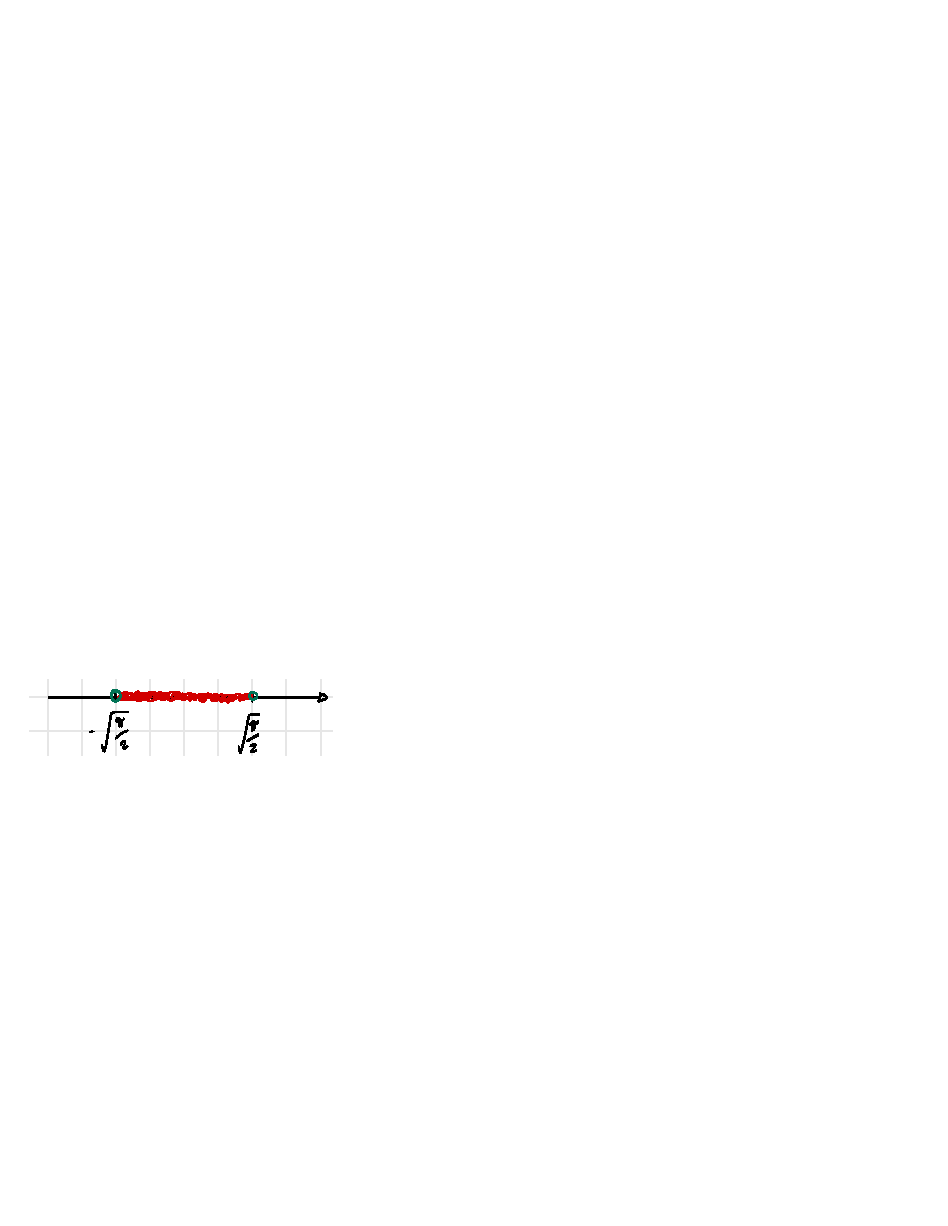
\includegraphics[width=0.7\textwidth]{img/intervallo_max_eg.pdf}
		\caption{Intervallo massimale delle soluzioni.}
	\end{figure}

	\newpage

	%%%%%%%%%%%%%%
	% LEZIONE 02 %
	%%%%%%%%%%%%%%
	\section{Lezione 02}
	
	\subsection[Problema di Cauchy per eq. diff. a variabili separabili]{Problema di Cauchy per equazioni differenziali a variabili separabili}
	
	Per introdurre il problema di Cauchy con le equazioni differenziali a variabili separabili, è necessario introdurre il \textbf{teorema di \underline{esistenza} e \underline{unicità}}.\newline
	
	\noindent
	Si consideri il problema:
	
	\begin{equation*}
		\begin{cases}
			y^{'} = f\left(x\right) \cdot g\left(y\right) \\
			y\left(x_{0}\right) = y_{0}
		\end{cases}
	\end{equation*}

	\noindent
	In cui $f$ è una funzione continua su $I = \left(x_{0} - r_{1}, x_{0} + r_{1}\right)$ e $g$ è una funzione continua su un intervallo $J = \left(y_{0} - r_{2}, y_{0} + r_{2}\right)$.
	
	\begin{theorem}[Esistenza]\label{teorema esistenza}
		Esiste una soluzione al problema di Cauchy definita per ogni $x \in I^{'} = \left[x_{0} - \delta, x + \delta\right] \subseteq I$. È dunque \textbf{garantita la soluzione locale} e non obbligatoriamente su tutto l'intervallo $I$.
	\end{theorem}

	\begin{theorem}[Unicità]\label{teorema unicità}
		Se $g\left(y\right)$ è \underline{continua e derivabile} con derivata continua (formalmente: $g\left(y\right) \in \mathcal{C}^{1} \left(J\right)$), allora la \textbf{soluzione è unica}.
	\end{theorem}

	\begin{figure}[!htp]
		\centering
		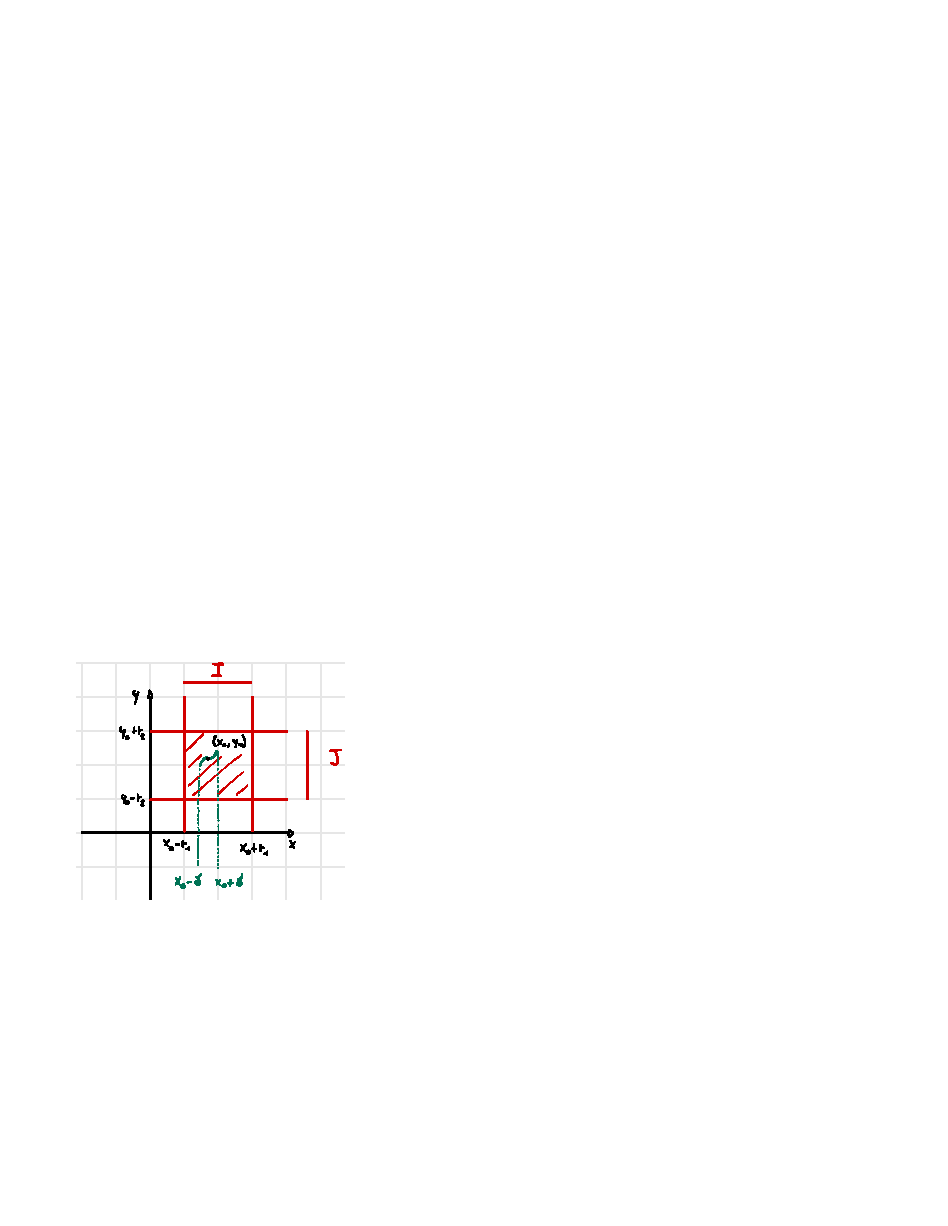
\includegraphics[width=0.8\textwidth]{img/prob_cauchy-variabili_separabili.pdf}
		\caption{Rappresentazione grafica del problema di Cauchy con variabili separabili.}
	\end{figure}

	\newpage

	\noindent
	\textbf{Caso in cui il teorema dell'unicità viene violato! È facilmente riconoscibile poiché ci sono due soluzioni che passano per la condizione imposta $\left(\text{il punto } x_{0}, y_{0}\right)$.}
	
	\begin{figure}[!htp]
		\centering
		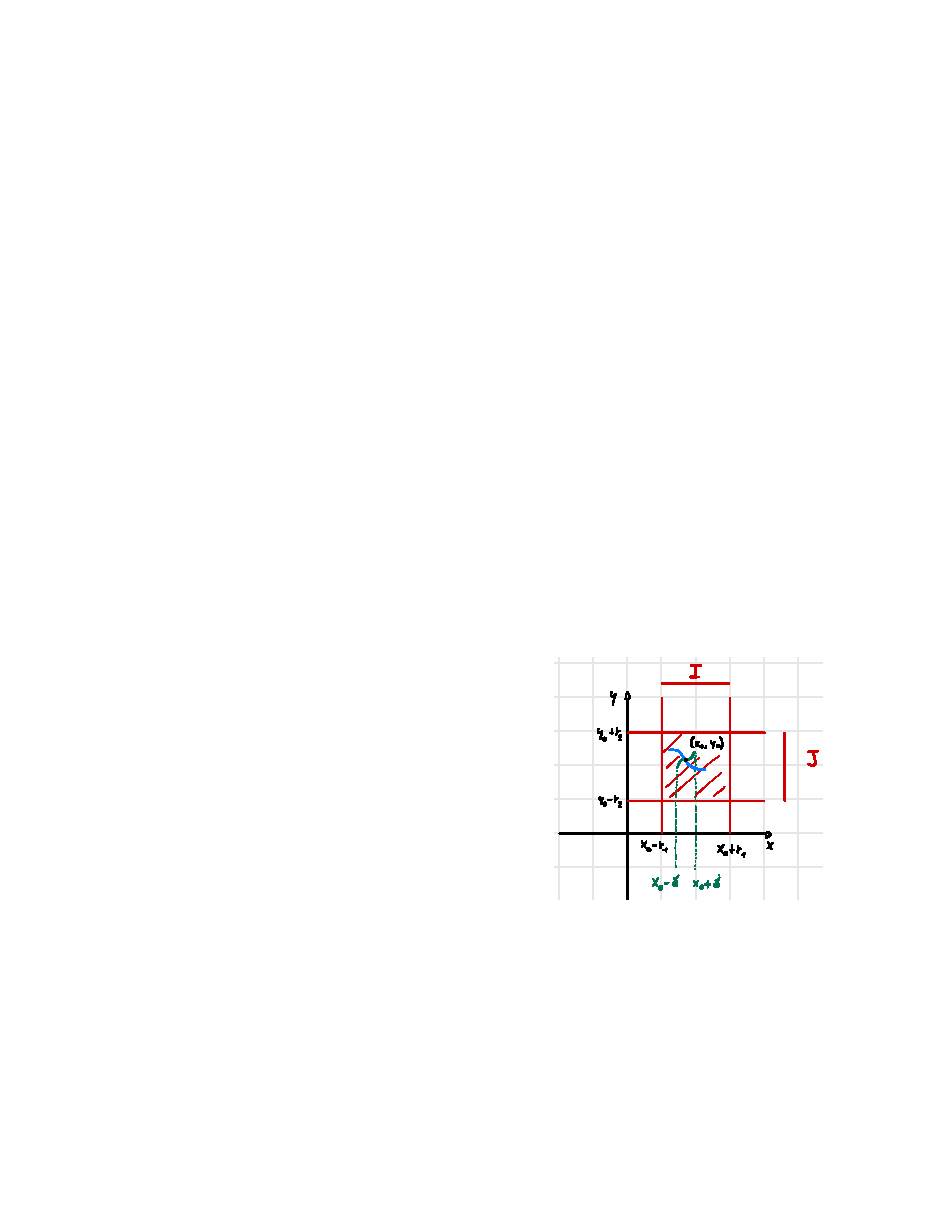
\includegraphics[width=0.8\textwidth]{img/prob_cauchy-variabili_separabili_violazione.pdf}
		\caption{Teorema dell'esistenza garantito, ma teorema dell'unicità violato.}
	\end{figure}

	\newpage
	
	\subsection{Esempi di problemi di Cauchy}
	
	\subsubsection[Esempio semplice]{\textcolor{Green4}{\textbf{Esempio semplice}}}
	
	\noindent
	Il problema:
	
	\begin{equation*}
		\begin{cases}
			y' \cdot y = 1 \\
			y\left(1\right) = 0
		\end{cases}
	\end{equation*}
	
	\noindent
	In questo caso \textbf{\underline{non esiste una soluzione}} poiché $y^{'}\left(1\right) \cdot y\left(1\right)$ deve essere uguale a $1$. Se nell'espressione $y^{'}\left(1\right) \cdot y\left(1\right) = 1$ vengono sostituite le funzioni con il valore zero, risulta impossibile l'uguaglianza: $y^{'}\left(1\right) \cdot 0 = 1$.\newline
	
	\subsubsection[Esempio medio]{\textcolor{Green4}{\textbf{Esempio medio}}}
	
	\noindent
	Il problema:
	
	\begin{equation*}
		\begin{cases}
			y' = y^{\frac{2}{3}} \\
			y\left(0\right) = 0
		\end{cases}
	\end{equation*}
	
	\noindent
	Esiste sicuramente \textbf{\underline{una soluzione costante}} con $y = 0$.
	
	Inoltre, andando a studiare le \textbf{\underline{soluzioni non costanti}}, quindi con $y \ne 0$, si evince chiaramente che:
	
	\begin{gather*}
		y^{'} = y^{\frac{2}{3}} \longrightarrow
		\dfrac{\mathrm{d}y}{y^{\frac{2}{3}}} = \mathrm{d}x \longrightarrow
		y^{-\frac{2}{3}} \mathrm{d}y = \mathrm{d}x \\
		\textbf{Integrando...} \longrightarrow
		3y^{\frac{1}{3}} = x + c
	\end{gather*}

	\noindent
	Dato che utilizzando la condizione del problema $y\left(0\right) = 0$ la $c$ è zero:
	
	\begin{equation*}
		3\left(y\left(0\right)^{\frac{1}{3}}\right) = 0 + c
	\end{equation*}

	\noindent
	Esplicitando la $y$, si ottiene la \textbf{soluzione al problema di Cauchy}:
	
	\begin{equation*}
		y = \dfrac{1}{27} x^{3} \hspace{2em} \text{con } x \ge 0
	\end{equation*}

	\newpage

	\noindent\fbox{%
		\parbox{\textwidth}{%
			È interessante notare che la soluzione può essere prolungata a tutto l'insieme dei reali $\mathbb{R}$:
			
			\begin{equation*}
				\tilde{y}\left(x\right) = 
				\begin{cases}
					0 					& x < 0 \\
					\dfrac{1}{27} x^{3} & x \ge 0
				\end{cases}
			\end{equation*}
		
			\noindent
			Inoltre, è possibile anche traslare funzioni di questo tipo:
			
			\begin{equation*}
				\tilde{y}\left(x\right) = 
				\begin{cases}
					0 & x < \alpha \\
					\dfrac{1}{27} \left(x - \alpha\right)^{3} & x \ge \alpha
				\end{cases}
			\end{equation*}
			
			\noindent
			Questo dimostra che la funzione ha una derivata non limitata nell'intervallo.
		}%
	}

	\begin{figure}[!htp]
		\centering
		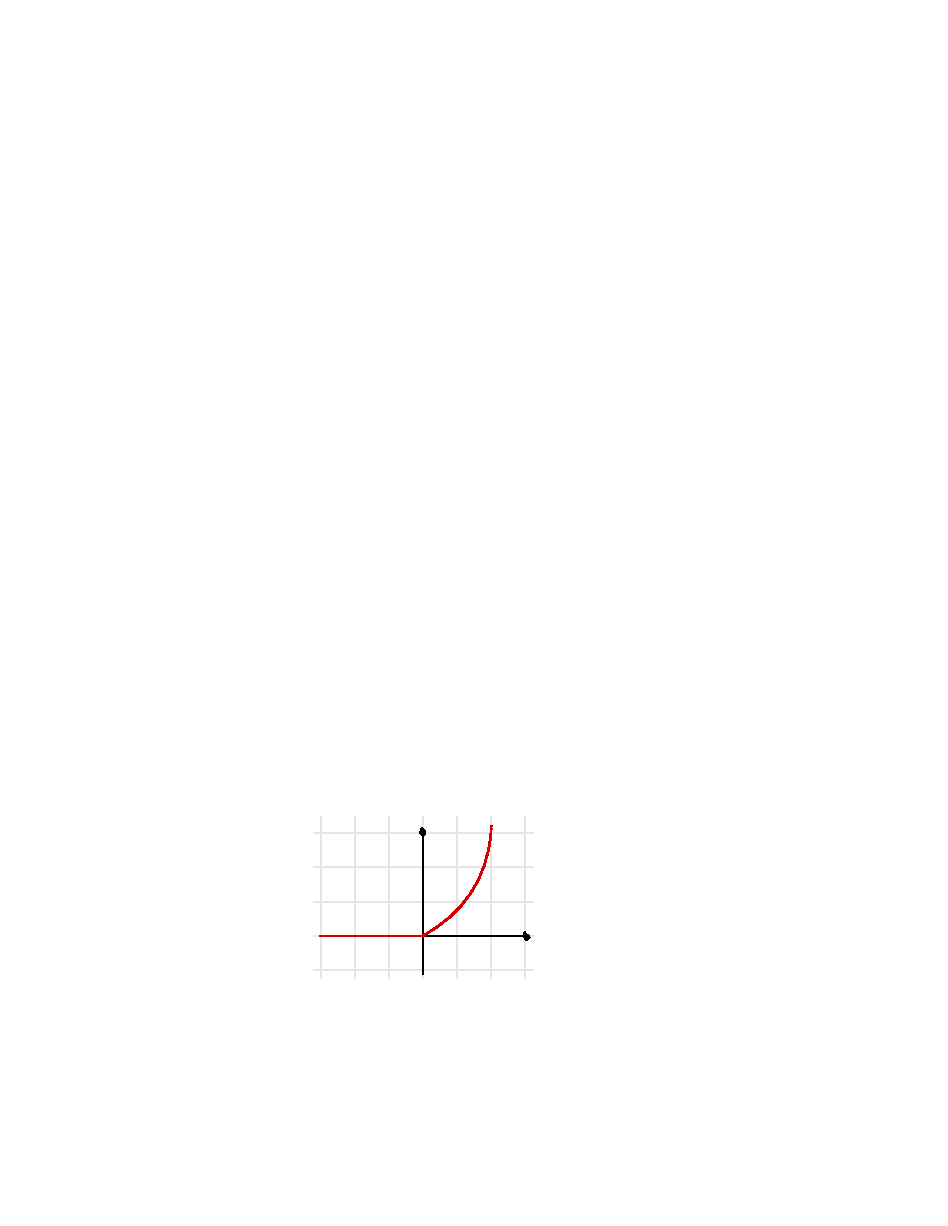
\includegraphics[width=0.6\textwidth]{img/prob_cauchy-variabili_separabili-OSS.pdf}
		\caption{Grafico dell'osservazione estesa a $\mathbb{R}$.}
		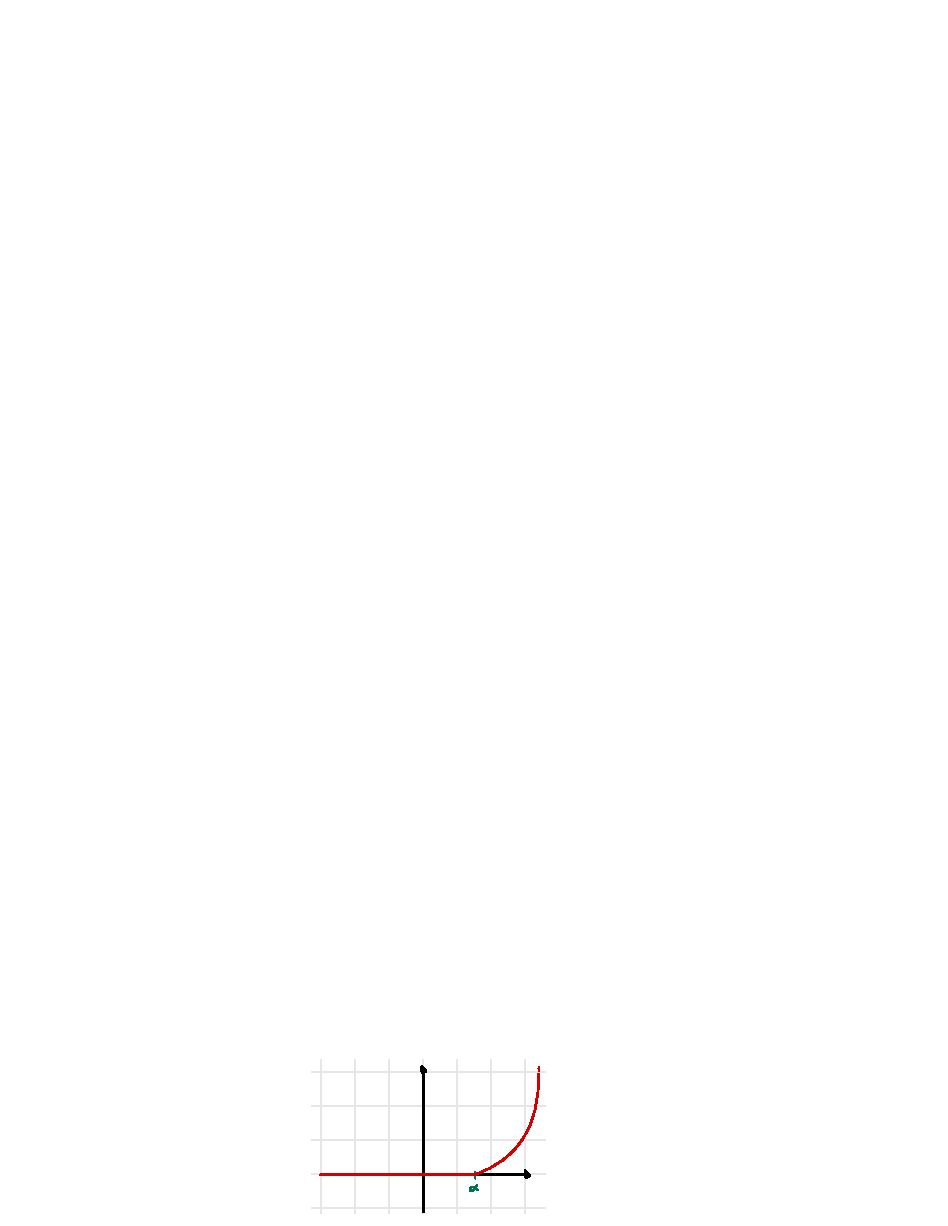
\includegraphics[width=0.6\textwidth]{img/prob_cauchy-variabili_separabili-OSS2.pdf}
		\caption{Grafico dell'osservazione estesa a $\mathbb{R}$ e traslata di $\alpha$.}
	\end{figure}

	\newpage
	
	\subsubsection[Esempio difficile]{\textcolor{Green4}{\textbf{Esempio difficile}}}
	
	\noindent
	Il problema:
	
	\begin{equation*}
		\begin{cases}
			e^{x+y} \cdot y + x = 0 \\
			y\left(0\right) = 0
		\end{cases}
	\end{equation*}
	
	\noindent
	Tuttavia, la funzione non è in forma canonica, quindi si eseguono alcune operazioni algebriche:
	
	\begin{equation*}
		e^{x+y} \cdot y + x = 0 \longrightarrow e^{x+y} \cdot y = -x \longrightarrow y^{'} = - \dfrac{x}{e^{x+y}}
	\end{equation*}

	\noindent
	Quindi:
	
	\begin{equation*}
		\begin{cases}
			y^{'} = - \dfrac{x}{e^{x+y}} \\
			y\left(0\right) = 0
		\end{cases}
	\end{equation*}

	\noindent
	Il problema si risolve tramite la \textbf{\underline{tecnica delle variabili separabili}}. Infatti:
	\begin{equation*}
		y^{'} = -\dfrac{x}{e^{x+y}}; \hspace{1em}
		y^{'} = -\dfrac{x}{e^{x} \cdot e^{y}}; \hspace{1em}
		y^{'} = -\dfrac{x}{e^{x}} \cdot \dfrac{1}{e^{y}}; \hspace{1em}
		y^{'} = - \underbracket[0.14ex]{x \cdot e^{-x}}_{f\left(x\right)} \cdot \underbracket[0.14ex]{e^{-y}}_{g\left(y\right)}
	\end{equation*}

	\noindent
	Con gli intervalli definiti in tutto $\mathbb{R}$ cioè $I = J = \mathbb{R}$.
	
	\noindent
	La risoluzione si svolge separando le variabili e integrando (N.B. la funzione $g\left(y\right)$ non ha zeri e quindi \textbf{\underline{non esistono soluzioni costanti}}):
	
	\begin{gather*}
		e^{y} \mathrm{d}y = -x e^{-x} \mathrm{d}x; \hspace{1em}
		\int e^{y} \mathrm{d}y = \int -x e{-x} \mathrm{d}x; \hspace{1em}
		e^{y} = x e^{-x} - \int 1 \cdot e^{-x} \mathrm{d}x; \hspace{1em} \\
		\textbf{Soluzione: } e^{y} = x e^{-x} + e^{-x} + c
	\end{gather*}

	\noindent
	Dunque, l'\textbf{\underline{integrale generale}}:
	
	\begin{equation*}
		y\left(x\right) = \ln \left(x e^{-x} + e^{-x} + c\right)
	\end{equation*}

	\noindent
	Imponendo la \textbf{condizione iniziale}:
	
	\begin{equation*}
		y\left(0\right) = \ln \left(1+c\right) \hspace{2em} \text{con } c = 0
	\end{equation*}

	\noindent
	Per cui, la \textbf{\underline{soluzione al problema di Cauchy}} è:
	
	\begin{equation*}
		y\left(x\right) = \ln\left(x e^{-x} + e^{-x}\right) \hspace{2em} \text{con } x > -1
	\end{equation*}

	\noindent
	L'\textbf{\underline{intervallo massimale}} è:
	
	\begin{equation*}
		\left(-1; +\infty\right)
	\end{equation*}

	\newpage
	
	\subsection{Modello di crescita logaritmica}
	
	Creato dal matematico belga Verhulst, riguarda le equazioni differenziali. Infatti, la forma generale trovata nei problemi di Cauchy è del tipo $y^{'} = a y \left(1 - by\right)$, ma in questo modello è importante una forma alternativa della funzione del problema di Cauchy:
	
	\begin{equation*}
		\begin{cases}
			\text{Funzione:} & y^{'} = k y \left(1 - y\right) \\
			\text{Condizione:} & y\left(0\right) = y_{0}
		\end{cases}
	\end{equation*}

	\noindent
	In modo più formale, nel modello di crescita logaritmica l'equazione differenziale rappresenta una frazione di popolazione. Dunque, è possibile riscriverla come:
	
	\begin{equation*}
		\begin{cases}
			y^{'} = k y\left(1 - y\right) & 0 \le y \le 1 \\
			y\left(0\right) = y_{0} & \text{altrimenti}
		\end{cases}
	\end{equation*}

	\noindent
	In questo caso, le \textbf{\underline{soluzioni costanti} (o stabili, o d'equilibrio)} sono $y = 0$ e $y = 1$. Invece, le \textbf{\underline{soluzioni \emph{non} costanti}} sono:
	
	\begin{gather*}
		\dfrac{\mathrm{d}y}{y\left(1 - y\right)} = k \mathrm{d}x \xlongrightarrow{\text{Integrando...}}
		\int \dfrac{\mathrm{d}y}{y\left(1 - y\right)} = \int k \mathrm{d}x; \\
		\ln\left(y\right) - \ln\left(1 - y\right) = k x + c; \\
		\ln\left(\dfrac{y}{1 - y}\right) = k x + c
	\end{gather*}

	\noindent
	Nonostante la forma sia corretta, è utile avere la $y$ esplicitata, quindi:
	
	\begin{gather*}
		\begin{matrix}
			\dfrac{y}{1 - y} = e^{kx} \cdot e^{c}; & y = e^{c} \cdot e^{kx} \cdot \left(1 - y\right); \\
			\\
			y = e^{c} \cdot e^{kx} - e^{c} \cdot e^{kx} y; & y\left(1 + e^{c} \cdot e^{kx}\right) = e^{c} \cdot e^{kx}; \\
			\\
			y\left(x\right) = \dfrac{e^{c} \cdot e^{kx}}{1 + e^{c} \cdot e^{kx}}
		\end{matrix}
	\end{gather*}

	\noindent
	Il modello si conclude \textbf{\underline{applicando}} la \textbf{\underline{condizione iniziale}}:
	
	\begin{gather*}
		\underbracket[0.14ex]{y\left(0\right)}_{=y_{0}} = \dfrac{e^{c}}{1 + e^{c}} \xlongrightarrow{\text{Esplicitando } e^{c}}
		\left(1 + e^{c}\right) y_{0} = e^{c}; \hspace{2em} e^{c} \left(y_{0} + 1\right) = y_{0}; \\
		e^{c} = \dfrac{y_{0}}{1 - y_{0}}
	\end{gather*}

	\newpage
	\noindent
	Quindi, andando a sostituire il valore trovato con la condizione iniziale, si trova la \textbf{\underline{soluzione}}:
	
	\begin{equation*}
		y\left(t\right) = \dfrac{\dfrac{y_{0}}{1 - y_{0}} \cdot e^{kx}}{1 + \dfrac{y_{0}}{1 - y_{0}} \cdot e^{kx}} = \dfrac{y_{0} \cdot e^{kx}}{1 - y_{0} + y_{0} \cdot e^{kx}}
	\end{equation*}

	\begin{figure}[!htp]
		\centering
		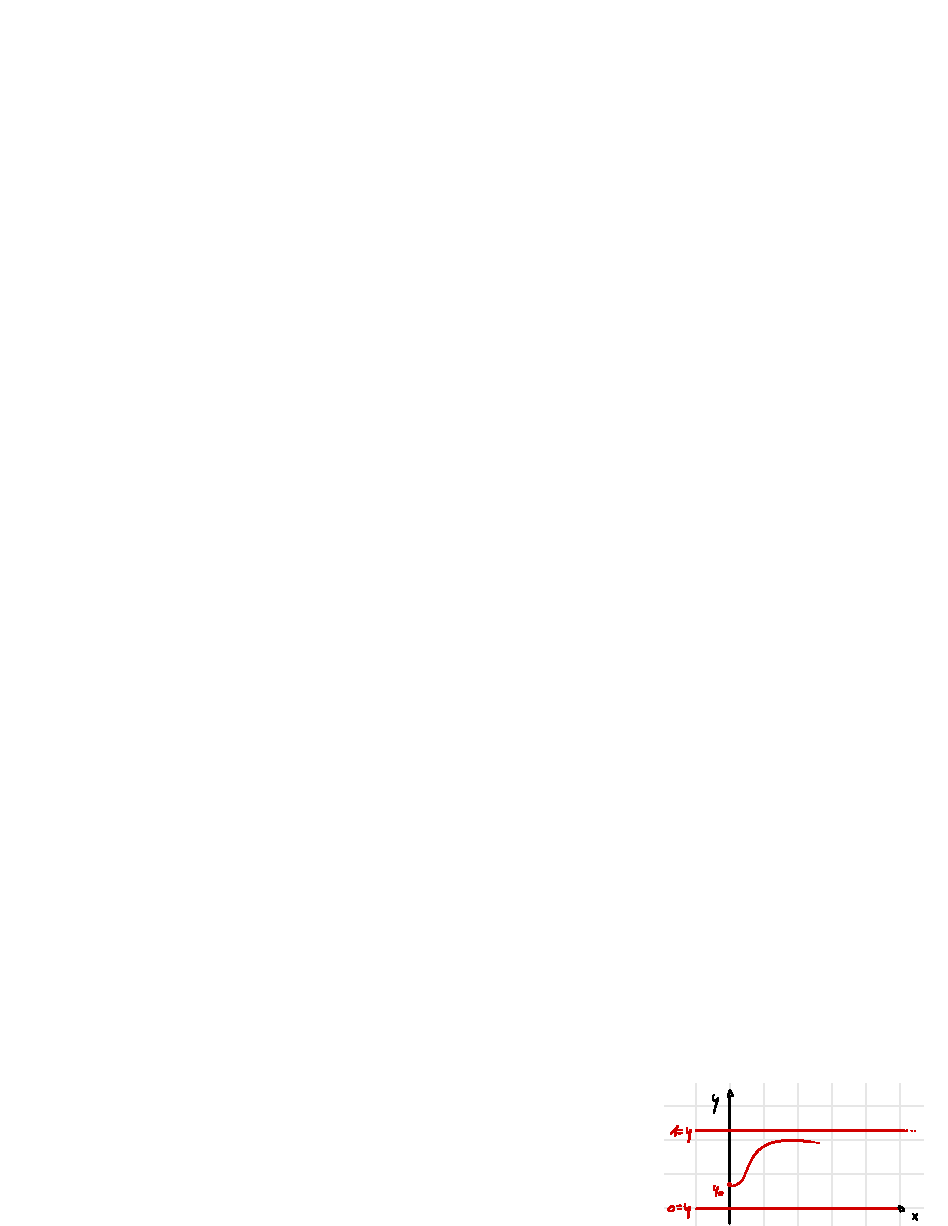
\includegraphics[width=0.7\textwidth]{img/modello_crescita_logaritmica-eg.pdf}
		\caption{Esempio di grafico con un certo $y_{0}$.}
	\end{figure}

	\newpage
	
	\subsection{Esercizio con domande da \textcolor{Red3}{esame}}
	
	Dato il seguente problema di Cauchy:
	
	\begin{equation*}
		\begin{cases}
			y^{'} = e^{x} + y^{2} \\
			y\left(0\right) = 1
		\end{cases}
	\end{equation*}

	\noindent
	Si \textbf{risponda alle seguenti \underline{domande}}:
	
	\begin{enumerate}[label=\Roman*.]
		\item Scrivere l'equazione della tangente al grafico della curva con soluzione nel punto di coordinate $\left(0, 1\right)$.
		
		\item Vicino (o intorno) al punto $x = 0$, la funzione è concava o convessa?
	\end{enumerate}
	
	\noindent
	\textcolor{Green4}{\textbf{\underline{Risposta domanda I.}}}\newline
	
	\noindent
	L'equazione generale (o definizione) della retta tangente è:
	
	\begin{equation*}
		y - y_{0} = m \left(x - x_{0}\right)
	\end{equation*}

	\noindent
	Con $x_{0}$, $y_{0}$ che sono coordinate del punto $m$, ovvero la \emph{pendenza}. Quindi, andando a sostituire le coordinate fornite dall'esercizio nella definizione di retta tangente:
	
	\begin{equation*}
		\textbf{Sostituzione } \left(0, 1\right) \rightarrow y - 1 = m \left(x - 0\right)
	\end{equation*}

	\noindent
	Sapendo che la pendenza $m$ è la derivata della funzione calcolata nel punto zero, si eseguono questi calcoli usando la funzione fornita dall'esercizio:
	
	\begin{equation*}
		m \longrightarrow y^{'}\left(0\right) = e^{0} + \left[y\left(0\right)\right]^{2}; \hspace{2em} y^{'}\left(0\right) = 1 + 1^{2} = 2
	\end{equation*}

	\noindent
	Il valore noto viene sostituito nella definizione di retta tangente, quindi l'equazione di quest'ultima diventa:
	
	\begin{equation*}
		y - 1 = 2\left(x - 0\right) \longrightarrow y = 2x - 1
	\end{equation*}\newline
	
	\noindent
	\textcolor{Green4}{\textbf{\underline{Risposta domanda II.}}}\newline
	
	\noindent
	Per la concavità o convessità si studia la derivata seconda:
	
	\begin{equation*}
		y^{''}\left(x\right) = e^{x} + 2y\left(x\right) \cdot y^{'}\left(x\right)
	\end{equation*}

	\noindent
	Dalla derivata seconda ottenuta si inserisce la condizione del problema:
	
	\begin{equation*}
		y^{''}\left(0\right) = 1 + 2 \cdot 1 \cdot \textcolor{Red3}{2} = 5
	\end{equation*}

	\noindent
	Il \textcolor{Red3}{2} è il risultato della $y^{'}\left(0\right)$ trovato prima.
	
	Dato che il \textbf{\underline{risultato è positivo, allora la funzione è convessa}}. Più formalmente, in un intorno di $x = 0$, se la $y^{''}\left(0\right) > 0$, la funzione si dice che è convessa.
	
	\section{Lezione 03}
	
	\subsection{Equazioni differenziali del primo ordine}
	
	La forma generale di un'equazione differenziale lineare del \textbf{\underline{primo ordine}} è la seguente:
	
	\begin{equation*}
		y^{'} + a\left(x\right) y = f\left(x\right) \hspace{2em} \text{con } a\left(x\right), f\left(x\right) \in \mathcal{C}^{0}\left(I\right)
	\end{equation*}

	\noindent
	Si ricorda che la $I$ indica l'intervallo nell'insieme dei numeri naturali $\mathbb{R}$. Inoltre, l'\textbf{equazione} si dice:
	
	\begin{itemize}
		\item \textcolor{Red3}{\textbf{\underline{Omogenea}}}, se $f\left(x\right) \equiv 0$, cioè è nulla;
		\item \textcolor{Red3}{\textbf{\underline{Non omogenea}}}, se $f\left(x\right) \not\equiv 0$, cioè non nulla;
	\end{itemize}

	\noindent
	La \textbf{\underline{risoluzione}} di queste equazioni prevede due passaggi:
	
	\begin{enumerate}
		\item Determinare una primitiva $A\left(x\right)$ di $a\left(x\right)$ sull'intervallo dei reali $I$ e considerare la funzione $e^{A\left(x\right)}$;
		
		\item Moltiplicare entrambi i membri dell'equazione differenziale per $e^{A\left(x\right)}$, chiamato anche \textcolor{Red3}{\textbf{\underline{fattore integrante}}}.
	\end{enumerate}

	\noindent
	L'\textcolor{Red3}{\textbf{\underline{obbiettivo}}} finale, ovvero successivamente alla risoluzione, è avere al primo membro la derivata di un prodotto tra funzioni.\newline
	
	\noindent
	Più esplicitamente, in maniera \textbf{generalistica}, si eseguono i seguenti passaggi:
	
	\begin{enumerate}
		\item $\overbrace{e^{A\left(x\right)} \cdot y^{'}\left(x\right) + e^{A\left(x\right)} \cdot a\left(x\right) \cdot y\left(x\right)}^{\text{Derivata di un prodotto tra due funzioni}} = e^{A\left(x\right)} \cdot f\left(x\right) \hspace{2em} \forall x \in I$

		\item $e^{A\left(x\right)} \cdot y\left(x\right) = \int e^{A\left(x\right)} f\left(x\right) \: \mathrm{d}x \hspace{2em} \text{con } c \in \mathbb{R}$
	\end{enumerate}

	\noindent
	Per derivata di un prodotto tra due funzioni ovviamente si intende:
	
	\begin{equation*}
		\left(e^{A\left(x\right)} \cdot y\left(x\right)\right)^{'}
	\end{equation*}

	\noindent
	La \textcolor{Red3}{\textbf{\underline{forma risolutiva generale}}} è la seguente:
	
	\begin{equation*}
		y\left(x\right) = e^{-A\left(x\right)} \left(\int e^{A\left(x\right)} f\left(x\right) \: \mathrm{d}x + c\right)
	\end{equation*}

	\noindent
	Ovviamente, per determinare la costante $c$ si utilizzano le condizioni iniziali.
	
	\newpage
	
	\noindent
	Combinando l'equazione differenziale lineare del primo ordine con le condizioni iniziali, il sistema da risolvere è il di nuovo il \textcolor{Red3}{\textbf{\underline{problema di Cauchy}}}:
	
	\begin{equation*}
		\begin{cases}
			y^{'}\left(x\right) + a\left(x\right) \cdot y\left(x\right) = f\left(x\right)	& a\left(x\right), f\left(x\right) \in \mathcal{C}^{0}\left(I\right) \\
			y\left(x_{0}\right) = y_{0}														& x_{0}, y_{0} \in I
		\end{cases}
	\end{equation*}

	\noindent
	E per definizione del teorema dell'esistenza e dell'unicità (teoremi \ref{teorema esistenza} e \ref{teorema unicità} a pagina \pageref{teorema esistenza}), l'equazione differenziale lineare del primo ordine \textbf{\underline{ammette un'unica soluzione}} \textbf{\underline{di classe}} $\mathcal{C}^{1}\left(I\right)$. Si osservi che la soluzione è definita su \emph{tutto} l'intervallo e di conseguenza è una \textbf{\underline{soluzione globale}}!\newline
	
	\noindent
	Nei prossimi paragrafi vengono presentati degli esempi guidati.
	
	\newpage
	
	\subsubsection[Esempio 1]{\textcolor{Green4}{\textbf{Esempio 1}}}
	
	L'equazione differenziale è la seguente:
	
	\begin{equation*}
		y^{'} + 2xy = x
	\end{equation*}

	\noindent
	Si osservi che l'equazione differenziale, oltre ad essere risolvibile tramite la tecnica presentata nel paragrafo precedente, è possibile risolverla anche a \emph{variabili separabili} (paragrafo \ref{Equazioni a variabili separabili}). In quest'ultimo caso, l'equazione sarebbe:
	
	\begin{equation*}
		y^{'} = x\left(1-2y\right)
	\end{equation*}

	\noindent
	Tuttavia, si ricerca l'integrale generale come spiegato nel metodo nel paragrafo precedente.\newline
	
	\noindent
	\textcolor{Red3}{\textbf{\underline{Passo 1}}}\newline
	
	\noindent
	Data la  forma generale dell'equazione differenziale lineare del primo ordine:
	
	\begin{equation*}
		y^{'} + a\left(x\right) y = f\left(x\right)
	\end{equation*}

	\noindent
	Dall'equazione dell'esercizio si ottiene:
	
	\begin{equation*}
		\begin{array}{lll}
			y^{'} + 2xy = x & \longrightarrow	& a\left(x\right) = 2x \\
							& \longrightarrow	& f\left(x\right) = x
		\end{array}
	\end{equation*}

	\noindent
	Con entrambe le funzioni $a\left(x\right)$ e $f\left(x\right)$ continue sull'insieme dei reali $\mathbb{R}$.\newline
	
	\noindent
	\textcolor{Red3}{\textbf{\underline{Passo 2}}}\newline
	
	\noindent
	Si calcola la primitiva del fattore $a\left(x\right)$:
	
	\begin{equation*}
		a\left(x\right) = 2x \xrightarrow{\text{primitiva}} A\left(x\right) = x^{2}
	\end{equation*}

	\noindent
	Così da costruire la funzione $e^{A\left(x\right)}$:
	
	\begin{equation*}
		e^{A\left(x\right)} \xrightarrow{\text{sostituzione}} e^{x^{2}}
	\end{equation*}

	\noindent
	Funzione chiamata anche \textbf{\underline{fattore integrante}}.\newline
	
	\noindent
	\textcolor{Red3}{\textbf{\underline{Passo 3}}}\newline
	
	\noindent
	Grazie al passo precedente si ha il fattore integrante, il quale viene usato per moltiplicare entrambi i membri dell'equazione differenziale. Quindi:
	
	\begin{equation*}
		\begin{array}{lllll}
			\text{Equazione differenziale}					& \longrightarrow & y^{'} + 2x \: y = x && \forall x \in \mathbb{R}\\
			\text{Equazione diff. per } e^{A\left(x\right)}	& \longrightarrow & \underbrace{e^{x^{2}} \cdot y^{'} + e^{x^{2}} \cdot 2x \: y}_{\left(e^{x^{2}} y\left(x\right)\right)^{'}} = e^{x^{2}} \cdot x && \forall x \in \mathbb{R}
		\end{array}
	\end{equation*}

	\newpage
	
	\noindent
	\textcolor{Red3}{\textbf{\underline{Passo 4}}}\newline
	
	\noindent
	Data la \textbf{\emph{forma risolutiva generale}} delle equazioni differenziali lineari del primo ordine:
	
	\begin{equation*}\label{eq}
		y\left(x\right) = e^{-A\left(x\right)} \left(\int e^{A\left(x\right)} f\left(x\right) \: \mathrm{d}x + c\right)
	\end{equation*}
	
	\noindent
	Si sostituiscono i valori noti e si calcola l'integrale:
	
	\begin{equation*}
		\begin{array}{lll}
			\text{Forma risolutiva generale}					& \longrightarrow & \text{(equazione sopra)} \\
			&& \\
			\text{Forma risolutiva generale con valori noti}	& \longrightarrow & e^{x^{2}} \cdot y\left(x\right) = \displaystyle \int x \cdot e^{x^{2}} \: \mathrm{d}x + c \\
			&& \\
																& \hookrightarrow & e^{x^{2}} \cdot y\left(x\right) = \dfrac{e^{x^{2}}}{2} + c \\
			&& \\
			\textbf{Integrale generale (forma finale)}			& \hookrightarrow & y\left(x\right) = \dfrac{1}{2} + c e^{-x^{2}}
		\end{array}
	\end{equation*}

	\noindent
	L'integrale generale ha sempre la $x$ nell'insieme dei reali ovviamente $x \in \mathbb{R}$.
	
	\newpage
	
	\subsubsection[Esempio 2]{\textcolor{Green4}{\textbf{Esempio 2}}}
	
	L'equazione differenziale è la seguente:
	
	\begin{equation*}
		y^{'} - \dfrac{1}{t} y = t^{2}
	\end{equation*}

	\noindent
	Si ricerca l'integrale generale.\newline
	
	\noindent
	\textcolor{Red3}{\textbf{\underline{Passo 1}}}\newline
	
	\noindent
	Data la forma generale dell'equazione differenziale lineare del primo ordine:
	
	\begin{equation*}
		y^{'} + a\left(x\right) y = f\left(x\right)
	\end{equation*}
	
	\noindent
	Si evidenziano i termini $a\left(x\right)$ e $f\left(x\right)$ nell'equazione differenziale dell'esercizio:
	
	\begin{equation*}
		\begin{array}{lll}
			y^{'} - \dfrac{1}{t} y = t^{2}	& \longrightarrow & a\left(t\right) = - \dfrac{1}{t} \\
											& \longrightarrow & f\left(t\right) = t^{2}
		\end{array}
	\end{equation*}

	\begin{center}
		\noindent
		\textcolor{Blue3}{\textbf{\underline{Attenzione!}}}
	\end{center}
	Si noti bene che in questo caso la $a\left(t\right)$ è definita nell'insieme: $\left(0, +\infty\right)$. Questo perché la funzione è una frazione e sicuramente non può essere una $0$. Inoltre, dato che \textbf{il problema di Cauchy si definisce solo su intervalli} e nel nostro caso la frazione sarebbe l'unione di due intervalli escluso lo $0$, cioè $\left(-\infty, 0\right) \cup \left(0, +\infty\right)$, è necessario scegliere quale intervallo utilizzare. La decisione viene presa in base ad una specifica dell'esercizio oppure, più frequentemente, in base al punto iniziale fornito dal problema di Cauchy. Infatti, se il punto iniziale fosse maggiore di $0$, si sceglierebbe l'intervallo $\left(0, +\infty\right)$, altrimenti, se fosse negativo, si sceglierebbe l'intervallo $\left(-\infty, 0\right)$.\newline
	
	\noindent
	Al contrario, la funzione $f\left(t\right)$ è definita nell'insieme dei reali $\mathbb{R}$.\newline
	
	\noindent
	\textcolor{Red3}{\textbf{\underline{Passo 2}}}\newline
	
	\noindent
	Si calcola la primitiva di $a\left(t\right)$ per costruire il fattore integrante. Quindi:
	
	\begin{equation*}
		a\left(t\right) = - \dfrac{1}{t} \xrightarrow{\text{primitiva}} A\left(t\right) = -\ln t
	\end{equation*}

	\noindent
	E di conseguenza il fattore integrante corrisponde a $e^{-\ln t}$. Con qualche accorgimento è possibile riscrivere il fattore integrante come:
	
	\begin{equation*}
		e^{-\ln t} = \dfrac{1}{t}
	\end{equation*}

	\noindent
	Il meno scompare perché si utilizza la proprietà fondamentale dei logaritmi e si ottiene $t^{-1}$.
	
	\newpage
	
	\noindent
	\textcolor{Red3}{\textbf{\underline{Passo 3}}}\newline
	
	\noindent
	Si esegue la moltiplicazione del fattore integrante per l'equazione differenziale:
	
	\begin{equation*}
		\begin{array}{lllll}
			\text{Equazione differenziale}					& \longrightarrow & y^{'} - \dfrac{1}{t} y = t^{2} && \\
			&&&& \\
			\text{Equazione diff. per } e^{A\left(x\right)}	& \longrightarrow & \underbrace{\dfrac{1}{t}y^{'} - \dfrac{1}{t^{2}}}_{\left(\dfrac{1}{t}y\left(t\right)\right)^{'}} = t && \text{con } t \in \left(0, +\infty\right)
		\end{array}
	\end{equation*}

	\noindent
	L'insieme in cui cade $t$ è definito nello stesso modo del passo 1.\newline

	\noindent
	\textcolor{Red3}{\textbf{\underline{Passo 4}}}\newline
	
	\noindent
	L'esercizio si conclude calcolando l'integrale generale tramite l'integrale vero e proprio:
	
	\begin{equation*}
		\begin{array}{rll}
			\dfrac{1}{t}y				& = &	\displaystyle\int t \: \mathrm{d}t + c \\
			&& \\
										& = &	\dfrac{1}{t}y = \dfrac{t^{2}}{2} + c \\
			&& \\
			\textbf{Integrale generale}	& = &	y\left(t\right) = \dfrac{1}{2} t^{3} + ct
		\end{array}
	\end{equation*}

	\noindent
	Con $t$ definita nell'insieme del passo 1, cioè $t \in \left(0, +\infty\right)$. Al contrario, la costante $c$ in tutto l'insieme dei reali, quindi $c \in \mathbb{R}$.
	
	\newpage
	
	\subsubsection[Esempio 3]{\textcolor{Green4}{\textbf{Esempio 3}}}
	
	L'equazione differenziale è la seguente:
	
	\begin{equation*}
		x^{'}\left(t\right) + \cot \left(t\right) x\left(t\right) = e^{t}
	\end{equation*}

	Si ricerca l'integrale generale.\newline
	
	\noindent
	\textcolor{Red3}{\textbf{\underline{Passo 1}}}\newline
	
	\noindent
	Talvolta le equazioni differenziali hanno variabili diverse dal solito, ma il ragionamento rimane invariato. In questo caso, l'equazione ha la variabile $t$ definita nell'intervallo $t \in \left(0, \pi\right)$. Il motivo è banale:
	
	\begin{equation*}
		\cot\left(t\right) = \dfrac{\cos\left(t\right)}{\sin\left(t\right)}
	\end{equation*}

	\noindent
	Data la forma generale dell'equazione differenziale lineare di primo grado:
	
	\begin{equation*}
		y^{'} + a\left(x\right) y = f\left(x\right)
	\end{equation*}

	\noindent
	Si evidenziano i termini $a\left(t\right)$ e $f\left(t\right)$ dall'equazione:
	
	\begin{equation*}
		\begin{array}{lll}
			x^{'}\left(t\right) + \cot \left(t\right) x\left(t\right) = e^{t}	& \longrightarrow & a\left(t\right) = \cot\left(t\right) \\
			& \longrightarrow & f\left(t\right) = e^{t}
		\end{array}
	\end{equation*}

	\noindent
	\textcolor{Red3}{\textbf{\underline{Passo 2}}}\newline
	
	\noindent
	Si calcola la primitiva di $a\left(t\right)$ così da ottenere il fattore integrante. Quindi:
	
	\begin{equation*}
		a\left(t\right) = \cot\left(t\right) \xrightarrow{\text{primitiva}} A\left(t\right) = \int\dfrac{\cos\left(t\right)}{\sin\left(t\right)} \: \mathrm{d}t = \ln \left|sin\left(t\right)\right|
	\end{equation*}
	
	\noindent
	Si sostituisce la primitiva nella definizione del fattore integrante $e^{A\left(t\right)}$ e si ottiene:
	
	\begin{equation*}
		e^{A\left(t\right)} \xrightarrow{\text{sostituzione}} e^{\ln\left|\sin\left(t\right)\right|} = \left|\sin\left(t\right)\right| = \sin\left(t\right)
	\end{equation*}
	
	\noindent
	È possibile portare il $\sin$ fuori dall'esponente grazie ad una delle proprietà dei logaritmi. Inoltre, grazie alla definizione dell'insieme in cui è definita $t$, cioè $t\in\left(0, +\infty\right)$, è possibile anche rimuovere il valore assoluto dato che sarà sempre positivo.\newline
	
	\noindent
	\textcolor{Red3}{\textbf{\underline{Passo 3}}}\newline
	
	\noindent
	L'equazione differenziale trovata al passo precedente viene moltiplicata per il fattore integrante:
	
	\begin{equation*}
		\begin{array}{lll}
			\text{Equazione differenziale}					& \longrightarrow & x^{'}\left(t\right) + \cot \left(t\right) x\left(t\right) = e^{t} \\
			&& \\
			\text{Equazione diff. per } e^{A\left(t\right)}	& \longrightarrow & \underbrace{\sin\left(t\right) \cdot x^{'}\left(t\right) + \cos\left(t\right) x\left(t\right)}_{\left(x\left(t\right) \cdot \sin\left(t\right)\right)^{'}} = e^{t} \cdot \sin\left(t\right)
		\end{array}
	\end{equation*}

	\noindent
	Il termine $\cos$ si ricava dall'operazione di moltiplicazione tra cotangente $\cot = \dfrac{\cos\left(t\right)}{\sin\left(t\right)}$ e il seno $\sin\left(t\right)$ che rappresenta il fattore integrante.
	
	\newpage
	
	\noindent
	\textcolor{Red3}{\textbf{\underline{Passo 4}}}\newline
	
	\noindent
	Si conclude l'esercizio trovando l'integrale generale:
	
	\begin{equation*}
		\begin{array}{lll}
			x\left(t\right) \cdot \sin\left(t\right) 	& = & \displaystyle\int e^{t} \sin\left(t\right) \: \mathrm{d}t \\
			&& \\
			\text{Integrale per parti}					& = & e^{t} \sin\left(t\right) - \displaystyle\int e^{t} \cos\left(t\right) \: \mathrm{d}t \\
			&& \\
			\text{Si ripete integrazione per parti}		& = & e^{t} \sin\left(t\right) - \left(e^{t} \cos\left(t\right) + \displaystyle\int e^{t} \sin\left(t\right) \: \mathrm{d}t \right) \\
			&& \\
														& = & e^{t} \sin\left(t\right) - e^{t} \cos\left(t\right) - \displaystyle\int e^{t} \sin\left(t\right) \: \mathrm{d}t
		\end{array}
	\end{equation*}

	\noindent
	Dato che l'incognita iniziale era l'integrale $\int e^{t} \sin\left(t\right) \: \mathrm{d}t$ e il risultato che è stato trovato corrisponde a $e^{t} \sin\left(t\right) - e^{t} \cos\left(t\right) - \displaystyle\int e^{t} \sin\left(t\right) \: \mathrm{d}t$, è possibile eguagliare questi due termini per ottenere la soluzione dell'integrale:
	
	\begin{equation*}
		\begin{array}{lll}
			\displaystyle\int e^{t} \sin\left(t\right) \: \mathrm{d}t	& = & e^{t} \sin\left(t\right) - e^{t} \cos\left(t\right) - \displaystyle\int e^{t} \sin\left(t\right) \: \mathrm{d}t \\
			&& \\
			\displaystyle\int e^{t} \sin\left(t\right) \: \mathrm{d}t + \displaystyle\int e^{t} \sin\left(t\right) \: \mathrm{d}t	& = & e^{t} \sin\left(t\right) - e^{t} \cos\left(t\right) \\
			&& \\
			2 \cdot \displaystyle\int e^{t} \sin\left(t\right) \: \mathrm{d}t & = & e^{t} \sin\left(t\right) - e^{t} \cos\left(t\right) \\
			&& \\
			\displaystyle\int e^{t} \sin\left(t\right) \: \mathrm{d}t 	& = & \dfrac{e^{t} \sin\left(t\right) - e^{t} \cos\left(t\right)}{2} \\
			&& \\
			\displaystyle\int e^{t} \sin\left(t\right) \: \mathrm{d}t 	& = & \dfrac{1}{2} \cdot e^{t} \left(\sin\left(t\right) - \cos\left(t\right)\right) + c
		\end{array}
	\end{equation*}

	\noindent
	Per concludere, si riprendere l'equazione generale iniziale e si sostituisce il risultato dell'integrale trovato:
	
	\begin{equation*}
		x\left(t\right) \cdot \sin\left(t\right) = \dfrac{1}{2} \cdot e^{t} \left(\sin\left(t\right) - \cos\left(t\right)\right) + c
	\end{equation*}

	\noindent
	Si esplicita l'incognita e si ottiene l'\textbf{integrale generale}:
	
	\begin{equation*}
		x\left(t\right) = \dfrac{1}{2} \cdot e^{t} \cdot \left(1 - \cot\left(t\right)\right) + \dfrac{c}{\sin\left(t\right)}
	\end{equation*}

	\newpage
	
	\subsection{Operatore differenziale lineare}
	
	Con un punto di vista ancora più generale, si definisce una particolare applicazione che si posiziona tra lo spazio continuo $\mathcal{C}^{1}\left(I\right)$ delle funzioni con derivata continua sull'intervallo $I$ e lo spazio continuo $\mathcal{C}^{0}\left(I\right)$ delle funzioni continue su $I$:
	
	\begin{equation}\label{operatore differenziale lineare di ordine 1}
		\begin{array}{llllll}
			L:	& \mathcal{C}^{1}\left(I\right) & \longrightarrow & \mathcal{C}^{0}\left(I\right) && \\
				& y\left(x\right)				& \longmapsto 	  & y^{'}\left(x\right) + a\left(x\right)y\left(x\right) && \text{con } a\left(x\right) \text{continua su } I
		\end{array}
	\end{equation}

	\noindent
	L'operazione definita e rappresentata dalla lettera $L$ si chiama: \textcolor{Red3}{\textbf{\underline{operatore}}} \textcolor{Red3}{\textbf{\underline{differenziale lineare di ordine 1}}}. Anche per questa operazione vale la \textbf{linearità}.\newline

	\noindent\fbox{%
		\parbox{\textwidth}{%
			\begin{center}
				\textcolor{Red3}{\textbf{\underline{Linearità}}}
			\end{center}
			
			\noindent
			Se $y_{1}\left(x\right), y_{2}\left(x\right) \in \mathcal{C}^{1}\left(I\right)$, allora l'operatore differenziale lineare di ordine 1 viene moltiplicato considerando anche le costanti:
			
			\begin{equation*}
				L\left(\alpha y_{1}\left(x\right) + \beta y_{2}\left(x\right)\right) = \alpha L\left(y_{1}\left(x\right)\right) + \beta L\left(y_{2}\left(x\right)\right) \hspace{2em} \text{con } \alpha, \beta \in \mathbb{R}
			\end{equation*}
			
			\noindent
			Quindi, l'equazione differenziale con la sua forma classica $y^{'}\left(x\right) + a\left(x\right) y\left(x\right) = f\left(x\right)$ con la funzione $f\left(x\right)$ continua sull'intervallo $I$, si può anche riscrivere come:
			
			\begin{equation*}
				L\left(y\left(x\right)\right) = f\left(x\right)
			\end{equation*}
		}%
	}

	\vspace{1.5em}

	\noindent
	Da questa definizione di linearità, la \textcolor{Red3}{\textbf{\underline{soluzione}}} cambia a seconda del tipo:
	
	\begin{itemize}[label=\ding{42}]
		\item \textcolor{Red3}{\textbf{\underline{Omogenea.}}} Allora la funzione $f\left(x\right) = 0$ e di conseguenza l'equazione differenziale $L\left(y\left(x\right)\right) = 0$ ovvero:
		\begin{equation*}
			v = \ker\left(L\right) \text{ è sottospazio vettoriale di } \mathcal{C}^{1}\left(I\right)
		\end{equation*}
		Dove:
		\begin{itemize}[label=-]
			\item $v$ rappresenta l'\textbf{insieme delle soluzioni} dell'omogenea associata;			
			\item $\ker\left(L\right)$ è il \textbf{nucleo} (\emph{kernel}, $\ker$) dell'\textbf{applicazione lineare} $L$;
			\item Il sottospazio vettoriale è chiaro, ma si ricordi che nel caso di equazioni differenziali del primo ordine, la \textbf{dimensione del sottospazio è pari a} $1$.
		\end{itemize}
		L'\textbf{\underline{obbiettivo}} delle soluzioni omogenee è trovare le funzioni di classe $\mathcal{C}^{1}$ che hanno come immagine un vettore nullo.
		
		\item \textcolor{Red3}{\textbf{\underline{Non omogenea.}}} L'insieme delle soluzioni dell'equazione differenziale $L\left(y\left(x\right)\right) = f\left(x\right)$ è definita come:
		\begin{equation*}
			\left\{y_{p}\left(x\right) + y_{v}\left(x\right) : y_{v}\left(x\right) \in \ker\left(L\right)\right\}
		\end{equation*}
	\end{itemize}

	\newpage

	\section{Lezione 04}
	
	\subsection{Equazioni differenziali lineari del secondo ordine}
	
	La forma generale di un'equazione differenziale lineare del \textbf{\underline{secondo ordine}} è la seguente:
	
	\begin{equation*}
		y^{''}\left(x\right) + a\left(x\right)y^{'}\left(x\right) + b\left(x\right)y\left(x\right) = f\left(x\right) \hspace{2em} \text{con } a\left(x\right), b\left(x\right), f\left(x\right) \in \mathcal{C}^{0}\left(I\right)
	\end{equation*}

	\noindent
	Solitamente le equazioni differenziali lineari del secondo ordine vengono associate ad un \textcolor{Red3}{\textbf{\underline{problema di Cauchy}}} date due condizioni iniziali. La forma generale:
	
	\begin{equation*}
		\begin{cases}
			y^{''}\left(x\right) + a\left(x\right)y^{'}\left(x\right) + b\left(x\right)y\left(x\right) = f\left(x\right) & a\left(x\right), b\left(x\right), f\left(x\right) \in \mathcal{C}^{0}\left(I\right) \\
			y\left(x_{0}\right) = y_{0} & x_{0} \in I \\
			y^{'}\left(x_{0}\right) = y_{1}
		\end{cases}
	\end{equation*}

	\noindent
	Anche per questo tipo di equazioni esiste il \textcolor{Red3}{\textbf{\underline{teorema di esistenza e unicità}}}: esiste ed è unica la soluzione al problema di Cauchy definita sull'intervallo $I$. La soluzione è definita in $\mathcal{C}^{2}\left(I\right)$.
	
	\vspace{2em}
	
	\subsubsection{Struttura dell'insieme delle soluzioni di un'equazione differenziale lineare del 2° ordine}
	
	Per l'insieme delle soluzioni si definisce un operatore differenziale lineare:
	
	\begin{equation*}
		\begin{array}{llll}
			L: 	& \mathcal{C}^{2}\left(I\right)	& \longrightarrow & \mathcal{C}^{0}\left(I\right) \\
				& y\left(x\right)				& \longmapsto	  & y^{''}\left(x\right) + a\left(x\right)y^{'}\left(x\right) + b\left(x\right)y\left(x\right) \hspace{2em} \text{con } a\left(x\right), b\left(x\right) \in \mathcal{C}^{0}\left(I\right)
		\end{array}
	\end{equation*}

	\noindent
	L'operatore differenziale lineare $L$ è considerato \dquotes{lineare} poiché:
	
	\begin{equation*}
		L\left(\alpha y_{1}\left(x\right) + f y_{2}\left(x\right)\right) = \alpha L\left(y_{1}\left(x\right)\right) + f L\left(y_{2}\left(x\right)\right) \hspace{2em} \text{con } \forall\alpha, f\in \mathbb{R}
	\end{equation*}

	\noindent
	Ne consegue che l'equazione differenziale e l'operatore differenziale lineare hanno una relazione:
	
	\begin{equation*}
		y^{''}\left(x\right) + a\left(x\right)y^{'}\left(x\right) + b\left(x\right)y\left(x\right) = f\left(x\right) \iff L\left(y\left(x\right)\right) = f\left(x\right)
	\end{equation*}

	\noindent
	\begin{theorem}
		L'insieme $V$ delle soluzioni dell'equazione lineare omogenea:
		
		\begin{equation*}
			y^{''}\left(x\right) + a\left(x\right)y^{'}\left(x\right) + b\left(x\right)y\left(x\right) = 0 \hspace{2em} \text{con } a\left(x\right), b\left(x\right) \in \mathcal{C}^{0}\left(I\right)
		\end{equation*}
	
		\noindent
		È uno spazio vettoriale di dimensione $2$.
	\end{theorem}

	\subsection{Equazioni differenziali lineari del secondo ordine omogenee a coefficienti costanti}
	
	\begin{theorem}
		La funzione $e^{\lambda x} \left(\lambda\in\mathbb{C}\right)$ è la soluzione dell'equazione omogenea $y^{''} + ay^{'} + by = 0$ con $a, b \in \mathbb{R}$ \underline{se e solo se} $\lambda$ è la soluzione dell'equazione algebrica di secondo grado $\lambda^{2} + a\lambda + b = 0$ (quest'ultima chiamata \textcolor{Red3}{\textbf{\underline{equazione caratteristica}}})
	\end{theorem}

	\noindent
	Sia $e^{\lambda x}$ una soluzione. Allora la derivata prima:
	
	\begin{equation*}
		y^{'}\left(x\right) = \lambda e^{\lambda x}
	\end{equation*}

	\noindent
	E la derivata seconda:
	
	\begin{equation*}
		y^{''}\left(x\right) = \lambda^{2} e^{\lambda x}
	\end{equation*}
	
	\noindent
	Sostituendo le derivate nell'equazione differenziale lineare di secondo grado:
	
	\begin{equation*}
		\begin{array}{llll}
			& \lambda^{2}e^{\lambda x} + a\lambda e^{\lambda x} + b e^{\lambda x}	& = & 0 \\
			&&& \\
			\longrightarrow & e^{\lambda x}	\underbrace{\left(\lambda^{2} + a\lambda + b\right)}_{\text{eq. caratteristica}}	& = & 0 \\
			&&& \\
			\text{La } e \text{ è sempre diverso da } 0: & \cancel{e^{\lambda x}} \left(\lambda^{2} + a\lambda + b\right) & = & 0
		\end{array}
	\end{equation*}

	\noindent
	La \textbf{\underline{risoluzione dell'equazione caratteristica}} prevede tre casi:
	
	\begin{enumerate}[label=\Roman*.]
		\item \textcolor{Red3}{\underline{\textbf{Caso} $\Delta > 0$.}} L'equazione caratteristica ha \textbf{due soluzioni reali distinte} $\lambda_{1}, \lambda_{2}$.\newline
		Quindi, $e^{\lambda_{1}x}$ e $e^{\lambda_{2}x}$ sono due soluzioni linearmente indipendenti dell'equazione omogenea.\newline
		Spazio soluzioni rappresenta l'\textbf{\underline{integrale generale}} $v = \left\{c_{1}e^{\lambda_{1}x} + c_{2}e^{\lambda_{2}x} : c_{1}, c_{2} \in \mathbb{R}\right\}$.
		
		\item \textcolor{Red3}{\underline{\textbf{Caso} $\Delta = 0$.}} L'equazione caratteristica ha \textbf{due soluzioni reali coincidenti} $\lambda_{1} = \lambda_{2}$.\newline
		Quindi, $e^{\lambda_{1}x}$ e $e^{\lambda_{2}x}$ sono due soluzioni linearmente indipendenti dell'equazione omogenea.\newline
		L'\textbf{\underline{integrale generale}} è così rappresentato: $y\left(x\right) = c_{1}e^{\lambda_{1}x} + c_{2}e^{\lambda_{2}x}$ con $c_{1}, c_{2} \in \mathbb{R}$.
		
		\item \textcolor{Red3}{\underline{\textbf{Caso} $\Delta < 0$.}} L'equazione caratteristica ha due soluzioni complesse coniugate $\lambda_{1,2} = \alpha \pm i\beta$.\newline
		Quindi, $e^{\left(\alpha + i\beta\right)x}$, $e^{\left(\alpha - i\beta\right)x}$ che grazie ad Eulero è possibile riscriverle:
		\begin{equation*}
			\begin{array}{lll}
				e^{\left(\alpha + i\beta\right)x}	& \longrightarrow & z_{1} = e^{\alpha x}\left(\cos\left(\beta x\right) + i \sin\left(\beta x\right)\right) \\
				&& \\
				e^{\left(\alpha - i\beta\right)x}   & \longrightarrow & z_{2} = e^{\alpha x}\left(\cos\left(\beta x\right) - i \sin\left(\beta x\right)\right)
			\end{array}
		\end{equation*}
		L'\textbf{\underline{integrale generale}} dunque risulta: $y\left(x\right) = c_{1}e^{\alpha x}\cos\left(\beta x\right) + c_{2}e^{\alpha x}\sin\left(\beta x\right)$
	\end{enumerate}

	\newpage

	\subsection{Equazioni differenziali complete omogenee a coefficienti costanti}
	
	L'\textbf{\underline{obbiettivo}} di questo tipo particolare di equazioni consiste nella \emph{ricerca di una soluzione particolare} (definizione spiegata qualche riga più avanti).
	
	La forma generale di un'equazione differenziale completa omogenea a coefficienti costanti è:
	
	\begin{equation*}
		y^{''} + ay^{'} + by = f\left(x\right) \hspace{2em} \text{con } x \in I
	\end{equation*}

	Per risolvere queste equazioni viene utilizzato il \textcolor{Red3}{\textbf{\underline{metodo di somiglianza}}}. Spiegato nel prossimo capitolo, esso consiste nell'individuare una somiglianza tra l'equazione differenziale da calcolare e una già calcolata.\newline
	
	\noindent
	Che cos'è una soluzione particolare? In generale, se la funzione $f\left(x\right)$ è un polinomio di grado $n$ tale che $\left(f\left(x\right) = P_{n}\left(x\right)\right)$ con $b \ne 0$, allora una soluzione particolare è un polinomio di grado $n$:
	
	\begin{equation*}
		y_{P}\left(x\right) = Q_{n}\left(x\right)
	\end{equation*}

	\noindent
	In cui $Q_{n}$ indica un polinomio di grado $n$.
	
	\newpage
	
	\section{Lezione 05}
	
	\subsection{Come trovare una soluzione particolare dell'equazione lineare del 2° ordine a coefficienti costanti}
	
	\begin{center}
		\large
		\textcolor{Red3}{\textbf{\underline{Metodo di somiglianza}}}
	\end{center}

	\noindent
	Se il termine forzante $f\left(x\right)$ ha una forma particolare, allora è possibile trovare una soluzione che abbia una forma \dquotes{simile} alla funzione $f\left(x\right)$:
	
	\begin{itemize}
		\item $f\left(x\right) = p\left(x\right) \cdot e^{\lambda x}$
		
		\item $f\left(x\right) = p\left(x\right) \cdot e^{\lambda x} \cdot \cos\left(\omega x\right)$
		
		\item $f\left(x\right) = p\left(x\right) \cdot e^{\lambda x} \cdot \sin\left(\omega x\right)$
	\end{itemize}

	\noindent
	Con $p$ che rappresenta il polinomio, invece le variabili $\alpha, \omega$ rappresentano numeri reali.
	
	\subsubsection[Esempio 1]{\textcolor{Green4}{Esempio 1}}
	
	Data l'equazione differenziale:
	
	\begin{equation*}
		y^{''} + 5y^{'} + 4y = 3 - 2x
	\end{equation*}
	
	\noindent
	L'obbiettivo è cercare un polinomio che abbia la forma del tipo:
	
	\begin{equation*}
		y_{p}\left(x\right) = a_{0} + a_{1}x
	\end{equation*}

	\noindent
	Nell'equazione differenziale, si nota bene che la parte $3-2x$ rappresenta il polinomio di 1° grado. Adesso si va a sostituire il polinomio $y_{P}$ nell'equazione differenziale ricordando di eseguire eventuali derivate:
	
	\begin{equation*}
		\begin{array}{lll}
			\text{Equazione differenziale} 	& \longrightarrow & y^{''} + 5y^{'} + 4y = 3 - 2x \\
			&& \\
			\text{Derivata seconda}			& \longrightarrow & y^{''} = \left(a_{0}+a_{1}x\right)^{''} = 0 \\
			&& \\
			\text{Derivata prima}			& \longrightarrow & 5y^{'} \\
			&& \\
											& \longrightarrow & 5\cdot\left(a_{0}+a_{1}x\right)^{'} \\
			&& \\
											& \longrightarrow & 5a_{1} \\
			&& \\
			\text{Equazione dopo aver sostituito} & \longrightarrow & 0 + 5a_{1} + 4\left(a_{0}+a_{1}x\right) = 3-2x \\
			&& \\
											& \longrightarrow & 5a_{1} + 4a_{0} + 4a_{1}x = 3 - 2x
		\end{array}
	\end{equation*}

	\noindent
	Con $\forall x \in \mathbb{R}$.

	\newpage

	\noindent
	Per capire se il polinomio è corretto bisogna eseguire un confronto. Quindi, per capire se due polinomi sono uguali, è necessario verificare che siano uguali i coefficienti. Si crea il sistema:
	
	\begin{equation*}
		\begin{cases}
			4a_{1} = -2 \\
			\\
			5a_{1} + 4a_{0} = 3
		\end{cases}
		\longrightarrow
		\begin{cases}
			a_{1} = -\dfrac{1}{2} \\
			\\
			a_{0} = \dfrac{11}{8}
		\end{cases}
	\end{equation*}

	\noindent
	Le equazioni inserite nel sistema corrispondono all'associazione effettuata nell'equazione differenziale, in particolare:
	
	\begin{equation*}
		\textcolor{Green4}{5a_{1}} + \textcolor{Green4}{4a_{0}} + \textcolor{Red3}{4a_{1}x} = \textcolor{Green4}{3} - \textcolor{Red3}{2x}
	\end{equation*}

	\noindent
	Grazie ai colori è adesso comprensibile la costruzione delle equazioni nel sistema:
	
	\begin{itemize}
		\item \textcolor{Green4}{\textbf{Verde}}: $5a_{1} + 4a_{0} = 3$
		\item \textcolor{Red3}{\textbf{Rosso}}: $4a_{1} = -2$
	\end{itemize}

	\noindent
	Dopo aver risolto il sistema, si riscrive il polinomio:
	
	\begin{equation*}
		y_{p} = \dfrac{11}{8} - \dfrac{1}{2}x
	\end{equation*}

	\noindent
	Si ottiene l'equazione caratteristica dall'equazione differenziale:
	
	\begin{equation*}
		y^{''} + 5y^{'} + 4y = 3 - 2x \longrightarrow \lambda^{2} + 5\lambda + 4 = 0
	\end{equation*}

	\noindent
	La quale ha due soluzioni reali distinte (dato che risale immediatamente all'occhio visto che il delta è positivo $\Delta > 0$) $\lambda_{1} = -4, \lambda_{2} = -1$.\newline
	
	\noindent
	Andando a creare l'equazione completa sommando i due fattori integranti e il polinomio:
	
	\begin{equation*}
		y\left(x\right) = c_{1}e^{-4x} + c_{2}e^{-x} + \dfrac{11}{8} - \dfrac{1}{2} x \hspace{2em} \text{con } c_{1}, c_{2} \in \mathbb{R}
	\end{equation*}

	\newpage
	
	\subsubsection[Esempio 2]{\textcolor{Green4}{Esempio 2}}
	
	Questo esempio è diverso dagli altri perché si divide in due casi che presentano ed evidenziano due situazioni differenti. L'idea sarebbe quella di svolgere i passaggi in modo coordinato, come se si stessero facendo nello stesso momento. Questo sarà il compito del lettore, ovvero quello di leggere i due casi nello stesso istante (magari alternando!)
	
	\begin{center}
		\large
		\textcolor{Green4}{\textbf{\underline{Caso A}}}
	\end{center}

	\noindent
	Data l'equazione differenziale:
	
	\begin{equation*}
		y^{''} - 3y^{'} +2y = e^{5x}
	\end{equation*}

	\noindent
	Il polinomio da ottenere è uguale a:
	
	\begin{equation*}
		y_{p}\left(x\right) = c \cdot e^{5x}
	\end{equation*}

	\noindent
	Prima di eseguire le sostituzioni nell'equazione differenziale, si effettuano le derivate:
	
	\begin{equation*}
		\begin{array}{lll}
			y_{p}^{'}\left(x\right)	& = & 5 \cdot c e^{5x} \\
			y_{p}^{''}\left(x\right)& = & 25 \cdot c e^{5x}
		\end{array}
	\end{equation*}

	\noindent
	Si effettua la sostituzione nell'equazione differenziale:
	
	\begin{equation*}
		\begin{array}{lll}
			\text{Equazione differenziale}	& \longrightarrow & y^{''} - 3y^{'} +2y = e^{5x} \\
			&& \\
			\text{Polinomio}				& \longrightarrow & y_{p}\left(x\right) = c \cdot e^{5x} \\
			&& \\
			\text{Derivate del polinomio}	& \longrightarrow & y_{p}^{'}\left(x\right)	= 5 \cdot c e^{5x} \\
			&& \\
											& \longrightarrow & y_{p}^{''}\left(x\right) = 25 \cdot c e^{5x} \\
			&& \\
			\text{Sostituzione}				& \longrightarrow & 25 \cdot c e^{5x} - 3 \left(5 \cdot c e^{5x}\right) + 2 \left(c \cdot e^{5x}\right) = e^{5x} \hspace{2em} \forall x \in \mathbb{R}
		\end{array}
	\end{equation*}

	\noindent
	Si eseguono alcune semplificazioni e si ottiene la variabile $c$:
	
	\begin{equation*}
		\begin{array}{rcc}
			\dfrac{25 \cdot c \cdot \cancel{e^{5x}}}{\cancel{e^{5x}}} - \dfrac{15 \cdot c \cdot \cancel{e^{5x}}}{\cancel{e^{5x}}} + \dfrac{2 \cdot c \cdot \cancel{e^{5x}}}{\cancel{e^{5x}}} & = & \dfrac{\cancel{e^{5x}}}{\cancel{e^{5x}}} \\
			&& \\
			25c - 15c + 2c & = & 1 \\
			&& \\
			c & = & \dfrac{1}{12}
		\end{array}
	\end{equation*}

	\noindent
	Quindi, il polinomio identificato inizialmente diventa:
	
	\begin{equation*}
		y_{p}\left(x\right) = c \cdot e^{5x} \longrightarrow y_{p}\left(x\right) = \dfrac{1}{12} e^{5x}
	\end{equation*}

	\noindent
	L'esercizio si conclude calcolando l'equazione caratteristica:
	
	\begin{equation*}
		\lambda^{2} - 3\lambda + 2 = 0
	\end{equation*}

	\noindent
	Le soluzioni dell'equazione di secondo grado sono due reali e distinte ($\Delta > 0$): $\lambda_{1} = 1, \lambda_{2} = 2$. Andando a sostituire le soluzioni all'interno dell'equazione completa, si ottiene:
	
	\begin{equation*}
		y\left(x\right) = c_{1}e^{x} + c_{2}e^{2x} + \dfrac{1}{12} e^{5x} \hspace{2em} \text{con } c_{1}, c_{2} \in \mathbb{R}
	\end{equation*}

	\noindent
	Si ricorda che l'equazione completa si costruisce sommando i due termini $c$ e le due $e$, le quali avranno come esponente la $x$ e come costante le soluzioni trovate nell'equazione caratteristica. Infine, si somma il polinomio trovato tramite la sostituzione del termine $c$. Quindi, evidenziando i termini:
	
	\begin{equation*}
		y\left(x\right) = \overbrace{c_{1}e^{x}}^{\lambda_{1}} + \underbrace{c_{2}e^{2x}}_{\lambda_{2}} + \overbrace{\dfrac{1}{12} e^{5x}}^{y_{p}}
	\end{equation*}

	\newpage
	
	\begin{center}
		\large
		\textcolor{Green4}{\textbf{\underline{Caso B}}}
	\end{center}
	
	\noindent
	Data l'equazione differenziale, differente dal caso precedente:
	
	\begin{equation*}
		y^{''} - 3y^{'} + 2y = e^{2x}
	\end{equation*}
	
	\noindent
	Il polinomio da ottenere è uguale a:
	
	\begin{equation*}
		y_{p}\left(x\right) = c \cdot e^{2x}
	\end{equation*}
	
	\noindent
	Prima di eseguire le sostituzioni nell'equazione differenziale, si effettuano le derivate:
	
	\begin{equation*}
		\begin{array}{lll}
			y_{p}^{'}\left(x\right)	& = & 2 \cdot c e^{2x} \\
			y_{p}^{''}\left(x\right)& = & 4 \cdot c e^{2x}
		\end{array}
	\end{equation*}
	
	\noindent
	Si effettua la sostituzione nell'equazione differenziale:
	
	\begin{equation*}
		\begin{array}{lll}
			\text{Equazione differenziale}	& \longrightarrow & y^{''} - 3y^{'} +2y = e^{2x} \\
			&& \\
			\text{Polinomio}				& \longrightarrow & y_{p}\left(x\right) = c \cdot e^{2x} \\
			&& \\
			\text{Derivate del polinomio}	& \longrightarrow & y_{p}^{'}\left(x\right)	= 2 \cdot c e^{2x} \\
			&& \\
			& \longrightarrow & y_{p}^{''}\left(x\right) = 4 \cdot c e^{2x} \\
			&& \\
			\text{Sostituzione}				& \longrightarrow & 4 \cdot c e^{2x} - 3 \left(2 \cdot c e^{2x}\right) + 2 \left(c \cdot e^{2x}\right) = e^{2x} \hspace{2em} \forall x \in \mathbb{R}
		\end{array}
	\end{equation*}
	
	\noindent
	Qui c'è la differenza sostanziale rispetto all'esercizio precedente. Provando a semplificare l'equazione differenziale tramite la variabile $e^{2x}$, si ottiene l'uguaglianza $0 = 1$:
	
	\begin{equation*}
		\dfrac{4 \cdot c \cdot \cancel{e^{2x}}}{\cancel{e^{2x}}} - \dfrac{3 \left(2 \cdot c \cdot \cancel{e^{2x}}\right)}{\cancel{e^{2x}}} + \dfrac{2 \left(c \cdot \cancel{e^{2x}}\right)}{\cancel{e^{2x}}} = \dfrac{\cancel{e^{2x}}}{\cancel{e^{2x}}}
	\end{equation*}

	\noindent
	Questo accade perché il valore $2$, il quale era l'unico termine diverso rispetto al caso A, è una soluzione dell'equazione caratteristica. Quindi, si cambia il polinomio applicando una piccola variazione:
	
	\begin{equation*}
		y_{p}\left(x\right) = c \cdot x \cdot e^{2x}
	\end{equation*}

	\noindent
	Si rieseguono i procedimenti classici:
	
	\begin{equation*}
		\begin{array}{lll}
			\text{Equazione differenziale}	& \longrightarrow & y^{''} - 3y^{'} +2y = e^{2x} \\
			&& \\
			\text{Polinomio}				& \longrightarrow & y_{p}\left(x\right) = c \cdot x \cdot e^{2x} \\
			&& \\
			\text{Derivate del polinomio}	& \longrightarrow & y_{p}^{'}\left(x\right)	= ce^{2x} + cx \cdot 2e^{2x} = ce^{2x}\left(1 + 2x\right) \\
			&& \\
			& \longrightarrow & y_{p}^{''}\left(x\right) = 2ce^{2x} \cdot \left(1 + 2x\right) + ce^{2x} \cdot 2 = 2ce^{2x}\left(2 + 2x\right) \\
			&& \\
			\text{Sostituzione}				& \longrightarrow & 2ce^{2x}\left(2 + 2x\right) - 3 \left(ce^{2x}\left(1 + 2x\right)\right) + 2\left(ce^{2x}\right) = e^{2x} \hspace{2em} \forall x \in \mathbb{R}
		\end{array}
	\end{equation*}

	\noindent
	Eseguendo le classe semplificazioni, che vengono omesse, si ottiene la costante uguale a $1$, $c = 1$. Si conclude l'esercizio andando a costruire il polinomio particolare:
	
	\begin{equation*}
		y_{p}\left(x\right) = x e^{2x}
	\end{equation*}

	\noindent
	Adesso si dovrebbe calcolare l'equazione caratteristica, trovare le sue soluzioni e andare a costruire l'equazione completa. Tuttavia, i passaggi sono identici al caso A dato che le due equazioni differenziali hanno i due termini a sinistra identici.
	
	\newpage
	
	\subsubsection[Esempio 3]{\textcolor{Green4}{Esempio 3}}
	
	Data l'equazione differenziale:
	
	\begin{equation*}
		y^{''} + y = \sin\left(2x\right)
	\end{equation*}

	Si calcola l'equazione particolare. Il polinomio simile è il seguente:
	
	\begin{equation*}
		y_{p}\left(x\right) = c_{1}\cos\left(2x\right) + c_{2}\sin\left(2x\right)
	\end{equation*}

	\noindent
	Si calcolano le derivate:
	
	\begin{equation*}
		\begin{array}{lll}
			y_{p}^{'}\left(x\right)	& = & -2c_{1}\sin\left(2x\right) + 2c_{2}\cos\left(2x\right) \\
			y_{p}^{''}\left(x\right)& = & -4c_{1}\cos\left(2x\right) - 4c_{2}\sin\left(2x\right)
		\end{array}
	\end{equation*}

	\noindent
	Nell'equazione differenziale si sostituiscono le derivate:
	
	\begin{equation*}
		-4c_{1}\cos\left(2x\right) - 3c_{2}\sin\left(2x\right) + c_{1}\cos\left(2x\right) + c_{2}\sin\left(2x\right) = \sin\left(2x\right)
	\end{equation*}

	\noindent
	Si eseguono le semplificazioni e si ottiene l'equazione:
	
	\begin{equation*}
		-3c_{1}\cos\left(2x\right) - 3c_{2}\sin\left(2x\right) = \sin\left(2x\right)
	\end{equation*}

	\noindent
	Le due costanti si ottengono inserendo i valori nel sistema:
	
	\begin{equation*}
		\begin{cases}
			-3c_{1} = 0 \\
			-3c_{2} = 1
		\end{cases}
		\longrightarrow
		\begin{cases}
			c_{1} = 0 \\
			c_{2} = -\dfrac{1}{3}
		\end{cases}
	\end{equation*}

	\noindent
	Si sostituiscono i valori trovati nel polinomio iniziale:
	
	\begin{equation*}
		y_{p}\left(x\right) = c_{1}\cos\left(2x\right) + c_{2}\sin\left(2x\right) \longrightarrow y_{p}\left(x\right) = -\dfrac{1}{3}\sin\left(2x\right)
	\end{equation*}

	\noindent\fbox{%
		\parbox{\textwidth}{%
			\textcolor{Red3}{\textbf{\underline{Attenzione!}}}\newline
			
			\noindent
			Nel caso in cui l'equazione differenziale fosse stata $y^{''} + y = \sin\left(x\right)$, la risoluzione avrebbe avuto gli stessi problemi dell'esempio 2, caso B. La situazione sarebbe stata risolto con una piccola variazione, ovvero aggiungendo una $x$ a $y_{p}$:
			
			\begin{equation*}
				\begin{array}{llll}
					\textcolor{Red3}{\textbf{OLD:}} & y_{p} & = & c_{1}\cos\left(x\right) + c_{2}\sin\left(x\right) \\
					\textcolor{Green4}{\textbf{NEW:}} & y_{p} & = & x \cdot \left(c_{1}\cos\left(x\right) + c_{2}\sin\left(x\right)\right)
				\end{array}
			\end{equation*}
		}%
	}

	\newpage
	
	\subsection{Sintesi}
	
	In questo capitolo è stato ampiamente spiegato come trovare una soluzione particolare per un'equazione differenziale lineare del 2° ordine a coefficienti costanti. Esistono alcune forme particolari che sono utili per trovare la soluzione (l'elenco è stato fatto all'inizio del capitolo). Il metodo di somiglianza funzione perché si suppone che la soluzione abbia una forma \dquotes{simile} alle forme particolari introdotte.
	
	Il primo esempio ha spiegato dettagliatamente i passaggi da seguire per risolvere questo tipo di esercizi. Il secondo ha introdotto un problema che è possibile che si verifichi, ovvero quello di trovare una soluzione dell'equazione caratteristica prima del previsto (caso B). Infine, il terzo esempio ha concluso la spiegazione mostrando un esercizio un leggermente più complesso.\newline
	
	\noindent
	Sia:
	
	\begin{equation*}
		f\left(x\right) = p\left(x\right) e^{\alpha x}
	\end{equation*}
	
	\noindent
	La funzione particolare, allora si costruisce l'equazione particolare in questo modo:
	
	\begin{equation*}
		y_{p}\left(x\right) = Q\left(x\right) x^{m} e^{\alpha x}
	\end{equation*}

	\noindent
	In cui la $Q$ rappresenta la $p$ nella funzione $f$. Invece, la variabile $m$ è la molteplicità di $\alpha$ come radice dell'equazione caratteristica e infatti è definita come $m\in\left\{0,1,2\right\}$.\newline
	
	\noindent
	Un'altra forma della funzione è:
	
	\begin{equation*}
		f\left(x\right) = p\left(x\right) e^{\alpha x} \cdot \underbrace{\cos\left(\omega x\right)}_{\text{oppure } \sin\left(\omega x\right)}
	\end{equation*}
	
	\noindent
	Allora la funzione particolare si costruisce in questo modo:
	
	\begin{equation*}
		y_{p}\left(x\right) = e^{\alpha x} \cdot x^{m} \left(Q_{1}\left(x\right)\cos\left(\omega x\right) + Q_{2}\left(x\right)\sin\left(\omega x\right)\right)
	\end{equation*}

	\noindent
	Con $m \ne 0$ se $\alpha + i \omega$ è la soluzione dell'equazione caratteristica.
	
	\newpage
	
	\section{Lezione 06}
	
	\subsection{Come trovare una soluzione particolare dell'equazione differenziale lineare del 2° ordine a coefficienti costanti}
	
	Oltre al metodo di somiglianza introdotto nel capitolo precedente, esiste un altro metodo chiamato \textbf{metodo di variazione delle costanti}.
	
	\noindent
	\textcolor{Red3}{\textbf{\underline{Metodo di variazione delle costanti}}}\newline
	
	\noindent
	Data l'equazione differenziale di secondo grado:
	
	\begin{equation*}
		y^{''} + ay^{'} + by = f\left(x\right)
	\end{equation*}

	\noindent
	È conosciuto l'integrale generale dell'omogenea associata $y_{v}\left(x\right) = c_{1}y_{1}\left(x\right) + c_{2}y_{2}\left(x\right)$ dove $y_{1}\left(x\right)$ e $y_{2}\left(x\right)$ sono soluzioni indipendenti su $I$.
	
	\noindent
	L'\textcolor{Red3}{\textbf{\underline{obbiettivo}}} è cercare una soluzione particolare dell'equazione completa nella forma:
	
	\begin{equation*}
		y_{p}\left(x\right) = c_{1}\left(x\right)y_{1}\left(x\right) + c_{2}\left(x\right)y_{2}\left(x\right)
	\end{equation*}

	\noindent
	Con $c_{1}, c_{2}$ sono variazioni delle costanti.\newline
	
	\noindent
	A \textbf{differenza del metodo di somiglianza}, le costanti qui sono \emph{funzioni}. Come nel metodo di somiglianza, l'equazione particolare si sostituisce nell'equazione completa calcolando le derivate (la seconda si omette perché sarà introdotta tra poco):
	
	\begin{equation*}
		\begin{array}{lll}
			y_{p}\left(x\right)		& = & c_{1}\left(x\right)y_{1}\left(x\right) + c_{2}\left(x\right)y_{2}\left(x\right) \\
			&& \\
			y_{p}^{'}\left(x\right) & = & c_{1}^{'}\left(x\right)y_{1}\left(x\right) + c_{1}\left(x\right)y_{1}^{'}\left(x\right) + c_{2}^{'}\left(x\right)y_{2}\left(x\right) + c_{2}\left(x\right)y_{2}^{'}\left(x\right)
		\end{array}
	\end{equation*}

	\noindent
	Per semplificare l'espressione, si esegue una scelta di comodo: $c_{1}^{'}\left(x\right)y_{1}\left(x\right) + c_{2}^{'}\left(x\right)y_{2}\left(x\right) = 0$ con $\forall x \in I$. Quindi, la derivata prima e seconda si \emph{riscrivono}:
	
	\begin{equation*}
		\begin{array}{lll}
			y_{p}^{'}\left(x\right)	& = & c_{1}\left(x\right)y_{1}^{'}\left(x\right) + c_{2}\left(x\right)y_{2}^{'}\left(x\right) \\
			&& \\
			y_{p}^{''}\left(x\right)& = & c_{1}^{'}\left(x\right)y_{1}^{'}\left(x\right) + c_{1}\left(x\right)y_{1}^{''}\left(x\right) + c_{2}^{'}\left(x\right)y_{2}^{'}\left(x\right) + c_{2}\left(x\right)y_{2}^{''}\left(x\right)
		\end{array}
	\end{equation*}

	\noindent
	Sostituendo e raggruppando le derivate nell'equazione completa, si ha:
	
	\begin{equation*}
		c_{1}\underbrace{\left( y_{1}^{''} + ay_{1}^{'} + by_{1} \right)}_{*} + c_{2}\underbrace{\left( y_{2}^{''} + ay_{2}^{'} + by_{2} \right)}_{*} + c_{1}^{'}y_{1}^{'} + c_{2}^{'}y_{2}^{'}
	\end{equation*}
	
	\noindent
	In cui le due equazioni tra parentesi contrassegnate con l'asterisco sono uguali a zero poiché vengono trattate solamente equazioni omogenee, cioè uguale a zero. Quindi, rimuovendo i termini nulli dall'equazione e mettendo a sistema i rimanenti:
	
	\begin{equation*}
		\cancel{c_{1}\left( y_{1}^{''} + ay_{1}^{'} + by_{1} \right)} + \cancel{c_{2}\left( y_{2}^{''} + ay_{2}^{'} + by_{2} \right)} + c_{1}^{'}y_{1}^{'} + c_{2}^{'}y_{2}^{'} \longrightarrow
		\begin{cases}
			c_{1}^{'}y_{1} + c_{2}^{'}y_{2} = 0 \\
			c_{1}^{'}y_{1}^{'} + c_{2}^{'}y_{2}^{'} = f\left(x\right)
		\end{cases}
	\end{equation*}

	\noindent
	Grazie al corso di algebra lineare è noto come scrivere un sistema in \textbf{forma matriciale}. In particolare si creano tre matrici, di cui la prima viene chiamata \textcolor{Red3}{\textbf{\underline{matrice wronskiana}}}:
	
	\begin{equation*}
		\begin{cases}
			c_{1}^{'}y_{1} + c_{2}^{'}y_{2} = 0 \\
			\\
			c_{1}^{'}y_{1}^{'} + c_{2}^{'}y_{2}^{'} = f\left(x\right)
		\end{cases}
		\longrightarrow
		\begin{bmatrix}
			y_{1} 		& y_{2} 	\\
						&			\\
			y_{1}^{'}	& y_{2}^{'}
		\end{bmatrix}
		\cdot
		\begin{bmatrix}
			c_{1}^{'} \\
			\\
			c_{2}^{'}
		\end{bmatrix}
		=
		\begin{bmatrix}
			0 \\
			\\
			f
		\end{bmatrix}
	\end{equation*}
	
	\noindent
	La \textbf{\underline{matrice wronskiana}} è associata a $y_{1}$ e $y_{2}$. Inoltre, è sempre invertibile $\forall x \in I$ cioè il \emph{determinante è diverso da zero}: $\det W\left(x\right) \ne 0$ $\forall x \in I$.\newline
	
	\noindent
	Grazie a questa forma matriciale, si calcolano le due variabili $c_{1}^{'}, c_{2}^{'}$:
	
	\begin{gather*}
		c_{1}^{'} = \dfrac{
		\begin{vmatrix}
			0	&	y_{2} 		\\
			f	& 	y_{2}^{'}
		\end{vmatrix}
		}{y_{1} \cdot y_{2}^{'} - y_{1}^{'} \cdot y_{2}}
		=
		- \dfrac{f \cdot y_{2}}{y_{1} \cdot y_{2}^{'} - y_{1}^{'} \cdot y_{2}}
		\\
		\\
		c_{1}^{'} = \dfrac{
		\begin{vmatrix}
			y_{1}		&	0	\\
			y_{1}^{'}	& 	f
		\end{vmatrix}
		}{y_{1} \cdot y_{2}^{'} - y_{1}^{'} \cdot y_{2}}
		=
		+ \dfrac{f \cdot y_{1}}{y_{1} \cdot y_{2}^{'} - y_{1}^{'} \cdot y_{2}}
	\end{gather*}

	\noindent
	Con $c_{1}^{'}$ e $c_{2}^{'}$ che sono continue nell'intervallo $I$ e quindi integrabili.
	
	\newpage
	
	\subsubsection[Esempio]{\textcolor{Green4}{Esempio}}
	
	Si risolva il seguente problema di Cauchy:
	
	\begin{equation*}
		\begin{cases}
			y'' + y = \sin\left(x\right) \\
			y\left(0\right) = 0 \\
			y'\left(0\right) = 0
		\end{cases}
	\end{equation*}

	\noindent
	Si elencano di seguito i passaggi per risolvere l'esercizio usando il metodo di variazione delle costanti (paragrafo precedente).\newline
	
	\noindent
	\textcolor{Red3}{\textbf{\underline{Passo 1}}}\newline
	
	\noindent
	Si ricava l'equazione caratteristica dall'equazione differenziale data:
	
	\begin{equation*}
		y'' + y = \sin\left(x\right) \longrightarrow \lambda^{2} + 1 = 0
	\end{equation*}

	\noindent
	Le soluzioni trovate sono due complesse coniugate: $\lambda_{1} = i, \lambda_{2} = -i$.\newline
	
	\noindent
	\textcolor{Red3}{\textbf{\underline{Passo 2}}}\newline
	
	\noindent
	Si scrive l'integrale generale dell'equazione differenziale omogenea associata, dato che è sicuro che esiste grazie alla matrice wronskiana: $y_{v}\left(x\right) = c_{1}\cos\left(x\right) + c_{2}\sin\left(x\right)$.\newline
	
	\noindent
	\textcolor{Red3}{\textbf{\underline{Passo 3}}}\newline
	
	\noindent
	Adesso è possibile costruire la matrice wronskiana:
	
	\begin{equation*}
		W\left(x\right) = \begin{bmatrix}
			\phantom{-}\cos\left(x\right)	&	\sin\left(x\right)	\\
			-\sin\left(x\right)				&	\cos\left(x\right)	
		\end{bmatrix}
		\text{ con } \det W\left(x\right) = \cos^{2}\left(x\right) + \sin^{2}\left(x\right) = 1 \hspace{2em} \forall x \in \mathbb{R}
	\end{equation*}
	
	\noindent
	In cui i valori nella seconda riga sono le derivate della prima.\newline
	
	\noindent
	\textcolor{Red3}{\textbf{\underline{Passo 4}}}\newline
	
	\noindent
	Si scrive l'intero sistema utilizzando le matrici:
	
	\begin{equation*}
		\begin{bmatrix}
			\phantom{-}\cos\left(x\right)	&	\sin\left(x\right) \\
			-\sin\left(x\right)				&	\cos\left(x\right)
		\end{bmatrix}
		\cdot
		\begin{bmatrix}
			c'_{1}\left(x\right) \\
			\\
			c'_{2}\left(x\right)
		\end{bmatrix}
		=
		\begin{bmatrix}
			0 \\
			\\
			\sin\left(x\right)
		\end{bmatrix}
	\end{equation*}

	\noindent
	E si calcola la matrice inversa:
	
	\begin{equation*}
		\begin{bmatrix}
			c'_{1}\left(x\right) \\
			\\
			c'_{2}\left(x\right)
		\end{bmatrix}
		=
		\underbrace{
			\begin{bmatrix}
				\cos\left(x\right)	&	-\sin\left(x\right) \\
				\sin\left(x\right)	&	\phantom{-}\cos\left(x\right)
			\end{bmatrix}
		}_{W^{-1}\left(x\right)}
		\cdot
		\begin{bmatrix}
			0 \\
			\\
			\sin\left(x\right)
		\end{bmatrix}
		=
		\begin{bmatrix}
			-\sin^{2}\left(x\right) \\
			\\
			\sin\left(x\right)\cos\left(x\right)
		\end{bmatrix}
	\end{equation*}

	\noindent
	Le costanti sono evidenti, ovvero:
	
	\begin{equation*}
		\begin{array}{lll}
			c'_{1}\left(x\right)	& = & -\sin^{2}\left(x\right) \\
			c'_{2}\left(x\right)	& = & \sin\left(x\right)\cos\left(x\right)
		\end{array}
	\end{equation*}

	\noindent
	\textcolor{Red3}{\textbf{\underline{Passo 5}}}\newline
	
	\noindent
	L'ultimo passaggio è calcolare l'integrale delle costanti trovate:
	
	\begin{equation*}
		\begin{array}{lllll}
			c_{1}\left(x\right) & = & \displaystyle-\int\sin^{2}\left(x\right)\:\mathrm{d}x & = & -\dfrac{1}{2}x + \dfrac{1}{4}\sin\left(2x\right) + c \\
			&&&& \\
			c_{2}\left(x\right) & = & \displaystyle\phantom{-}\int\sin\left(x\right)\cos\left(x\right)\:\mathrm{d}x & = & -\dfrac{1}{4}\cos\left(2x\right) + c
		\end{array}
	\end{equation*}

	\noindent
	Andando a sostituire le soluzioni trovate nell'equazione particolare $y_{p}$ si trovano i valori:
	
	\begin{equation*}
		\begin{array}{lll}
			y_{p}\left(x\right) & = & c_{1}\left(x\right)\cos\left(x\right) + c_{2}\left(x\right)\sin\left(x\right) \\
			&& \\
								& = & \left(- \dfrac{1}{2}x + \dfrac{1}{4} \sin\left(2x\right)\right)\cos\left(x\right) - \dfrac{1}{4} \cos\left(2x\right)\sin\left(x\right)
		\end{array}
	\end{equation*}
	
	\newpage
	
	\section{Lezione 07}
	
	\subsection[Spazio euclideo ${n}$-dimensionale]{Spazio euclideo $\boldsymbol{n}$-dimensionale}
	
	L'insieme in cui si lavora è il seguente:
	
	\begin{equation*}
		\mathbb{R}^{n} = \left\{x = \left(x_{1}, x_{2}, ..., x_{n}\right) : x_{i} \in \mathbb{R}\right\} \hspace{2em} \text{con } i \in \mathbb{N}, 1 \le i \le n
	\end{equation*}

	\noindent
	Che identifica uno \textbf{\underline{spazio vettoriale normato}}.\newline
	
	\noindent
	\textcolor{Red3}{\textbf{\underline{Ripasso - Spazio vettoriale:}}} nello spazio vettoriale esistono due operazioni:
	
	\begin{itemize}
		\item \textbf{Somma:} $\left(x_{1}, ..., x_{n}\right) + \left(y_{1}, ..., y_{n}\right) = \left(x_{1} + y_{1}, x_{2} + y_{2}, ..., x_{n} + y_{n}\right)$ con $x,y \in \mathbb{R}^{n}$
		
		\item \textbf{Prodotto per uno scalare:} $\lambda \in \mathbb{R}, x = \left(x_{1}, ..., x_{n}\right) \in \mathbb{R}^{n} : \lambda x = \left(\lambda x_{1}, \lambda x_{2}, ..., \lambda x_{n}\right)$
	\end{itemize}
	\:\newline

	\noindent
	\textcolor{Red3}{\textbf{\underline{Ripasso - Normato:}}} lo spazio vettoriale è normato quando è dotato di una norma, ovvero di una funzione particolare in $\mathbb{R}^{n}$: \textbf{dominio} $\Big||\cdot|\Big| : \mathbb{R}^{n} \longrightarrow \mathbb{R}$, ovvero un vettore restituisce un numero reale:
	
	\begin{equation*}
		x \longmapsto \Big||x|\Big| \text{ che sarebbe la norma di } x
	\end{equation*}

	\noindent
	Le sue caratteristiche sono:
	
	\begin{itemize}
		\item $\Big|x\Big| \ge 0$, la norma di x è maggiore uguale a zero per ogni $x \in \mathbb{R}^{n}$; inoltre la norma di $x$ è zero $\Big||x|\Big| = 0$ (norma che rappresenta un numero reale) se e solo se $x = 0$ (con $x$ che è un vettore in $\mathbb{R}^{n}$).
		
		\item $\Big||\lambda x|\Big| = |\lambda| \Big||x|\Big|$, ovvero i vettori sono uguali ad un numero reale per un vettore. Questo vale per ogni $\lambda \in \mathbb{R}$ e per ogni $x \in \mathbb{R}^{n}$.
		
		\item $\Big||x+y|\Big| \le \Big||x|\Big| + \Big||y|\Big|$ per ogni $x,y \in \mathbb{R}^{n}$. Caratteristica chiamata \textcolor{Red3}{\textbf{\underline{disuguaglianza triangolare}}}.
	\end{itemize}

	\newpage
	
	\subsection{Norma euclidea}
	
	Si definisce la Norma Euclidea una norma di uno spazio vettoriale, quindi quello che è già stato affrontato nel paragrafo precedente:
	
	\begin{equation}\label{Norma euclidea}
		\Big||x|\Big|_{2} = \sqrt{\sum_{i = 1}^{n} x_{i}^{2}} = \sqrt{x \cdot x}
	\end{equation}
	
	\noindent
	In cui la moltiplicazione rappresenta il prodotto scalare nell'insieme $\mathbb{R}^{n}$.
	
	\subsection{Disuguaglianza (triangolare) di Cauchy-Schwarz}
	
	Per ogni $x, y \in \mathbb{R}^{n}$ si ha:
	
	\begin{equation}\label{disuguaglianza triangolare di cauchy-schwarz}
		|x \cdot y| \le \Big||x|\Big| \cdot \Big||y|\Big|
	\end{equation}

	\noindent
	In cui il termine di sinistra indica il prodotto scalare assoluto tra due vettori, mentre il termine di destra indica il prodotto nell'insieme $\mathbb{R}$ di norme tra due vettori.
	
	\subsection{Distanza euclidea}
	
	Introdotta dalla norma seconda, si definisce la distanza euclidea come:
	
	\begin{equation}\label{distanza euclidea}
		\mathrm{d}\left(x,y\right) = \Big||x-y|\Big| = \sqrt{\left(x_{1}-y_{1}\right)^{2} + \left(x_{2}-y_{2}\right)^{2} + \cdots + \left(x_{1}-y_{1}\right)^{2}} \hspace{2em} \text{con } x,y\in\mathbb{R}^{n}
	\end{equation}

	\noindent
	Come si vede sotto la radice, essa non è altro che la \emph{differenza delle varie componenti dei vettori}.

	\noindent
	Per completezza si introduce anche la definizione di \textbf{\underline{distanza di Manhattan}}:
	
	\begin{equation}\label{distanza di Manhattan}
		\mathrm{d}_{1}\left(x,y\right) = \Big||x-y|\Big|_{1} = \sum_{i = 1}^{n} |x_{i} - y_{i}|
	\end{equation}

	\noindent
	Inoltre, si definisce \textbf{\underline{metrica}} una funzione $\mathrm{d}$ in $\mathbb{R}^{n}$:
	
	\begin{equation}\label{metrica}
		\begin{array}{lll}
			\mathbb{R}^{n} \times \mathbb{R}^{n} & \longrightarrow & \mathbb{R} \\
			&& \\
			\left(x,y\right)					 & \longmapsto	   & \mathrm{d}\left(x,y\right)
		\end{array}
	\end{equation}

	\noindent
	Con le seguenti \textbf{\emph{proprietà}}:
	
	\begin{itemize}
		\item \textbf{Non negatività:} $\mathrm{d}\left(x,y\right) \ge 0$ per ogni $x,y$. Inoltre, $\mathrm{d}\left(x,y\right) = 0$ se e solo se $x = y$ (la distanza tra $x$ e $y$ non è \underline{mai} nulla).
		
		\item \textbf{Simmetria:} $\mathrm{d}\left(x,y\right) = \mathrm{d}\left(y,x\right)$ per ogni $x,y\in\mathbb{R}^{n}$ (la distanza deve essere una funzione simmetrica).
		
		\item \textbf{Disuguaglianza triangolare:} $\mathrm{d}\left(x,y\right) + \mathrm{d}\left(y,z\right) \ge \mathrm{d}\left(x,z\right)$ per ogni $x,y,z \in \mathbb{R}^{n}$ (disuguaglianza triangolare).
	\end{itemize}

	\newpage
	
	\subsection{Topologia in $\mathbb{R}^{n}$}
	
	Si definisce la \textbf{palla aperta} di centro $\bar{x}\in\mathbb{R}^{n}$ e raggio maggiore di zero $r > 0$, cioè la distanza è minore del raggio $r$. La funzione è definita in questo modo:
	
	\begin{equation*}
		B_{r}\left(\bar{x}\right) = \left\{x \in \mathbb{R}^{n} : \mathrm{d}\left(x,\bar{x}\right) < r\right\}
	\end{equation*}

	\noindent
	Un esempio di palla aperta con $n = 2$:
	
	\begin{figure}[!htp]
		\centering
		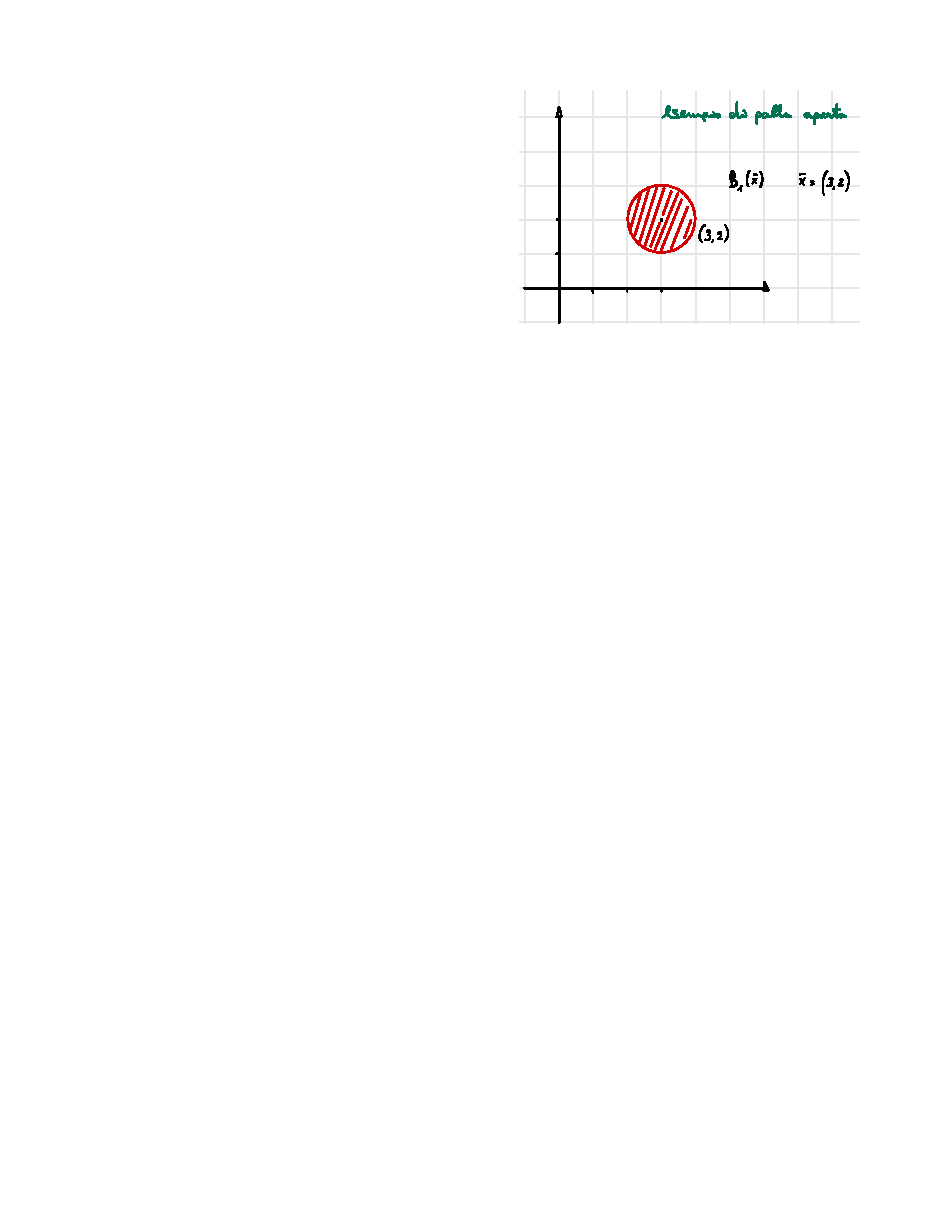
\includegraphics[width=0.6\textwidth]{img/palla_aperta.pdf}
		\caption{Palla aperta di coordinate $\left(3,2\right)$ con $n = 2$.}
	\end{figure}

	\noindent
	Con $n = 1$ la dimensione è monodimensionale:
	
	\begin{figure}[!htp]
		\centering
		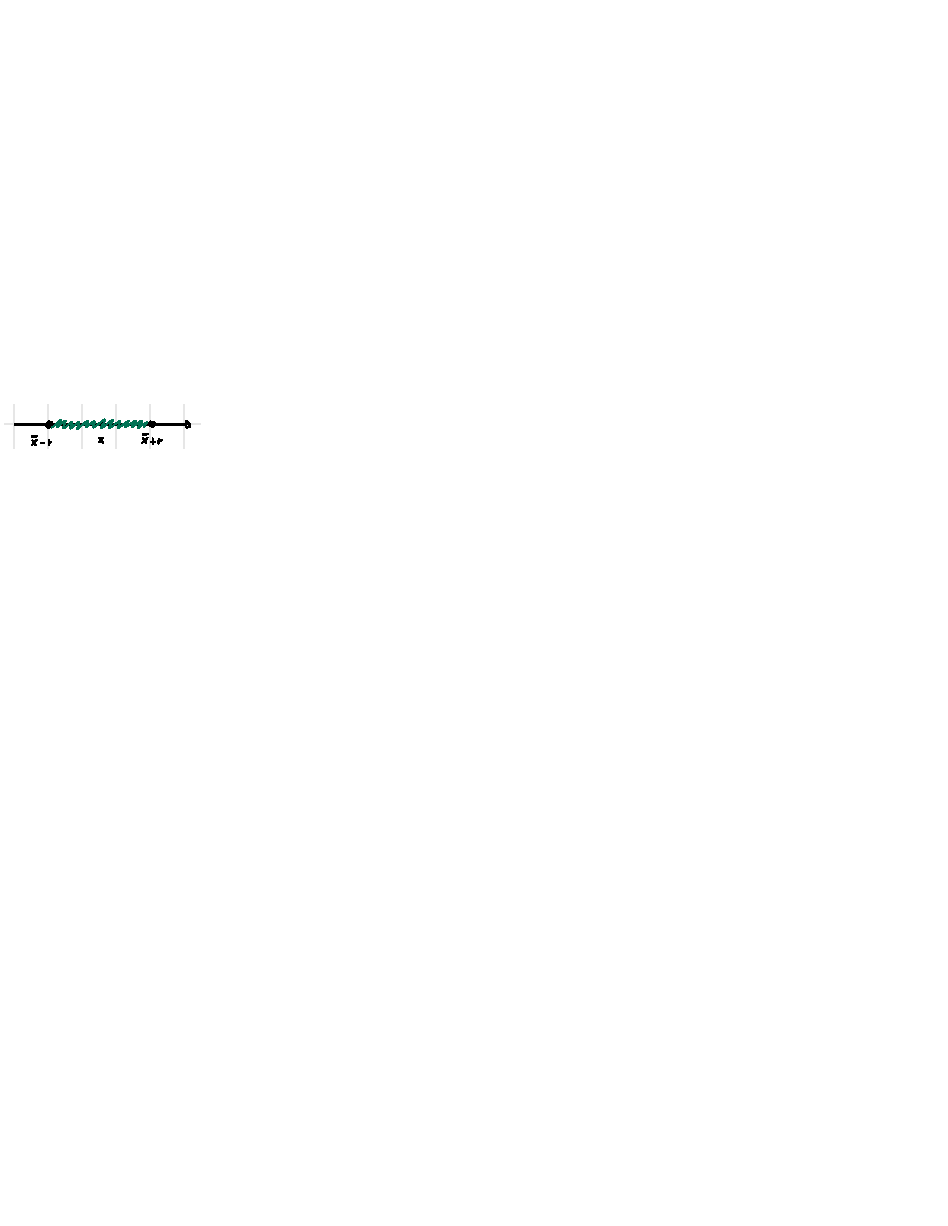
\includegraphics[width=0.5\textwidth]{img/monodimensionale.pdf}
		\caption{Retta monodimensionale con $n = 1$.}
	\end{figure}

	\noindent
	Con $n = 3$ la dimensione è tridimensionale:
	
	\begin{figure}[!htp]
		\centering
		\includegraphics[width=0.5\textwidth]{img/tridimensionale.pdf}
		\caption{Sfera in $\mathbb{R}$ con $n = 3$ senza bordo, cioè senza superficie.}
	\end{figure}

	\newpage
	
	\noindent\fcolorbox{Red3}{white}{%
		\parbox{\textwidth}{%
			\textcolor{Red3}{\textbf{\underline{Definizione}}}\newline
			
			\noindent
			Si definisce $U$ come il sottoinsieme di $\mathbb{R}^{ n}$, cioè $U \subseteq \mathbb{R}^{n}$ che è intorno di $\bar{x} \in \mathbb{R}^{n}$ se esiste $\exists r > 0$ tale che la palla è centrata: $B_{r}\left(\bar{x}\right) \subseteq U$
		}%
	}
	\:\newline

	\noindent
	\textcolor{Green4}{\textbf{Per esempio}}, data la seguente figura, si determini se:
	
	\begin{enumerate}
		\item $U$ è intorno di $v = \left(1,1\right)$?
		
		\item $U$ è intorno di $v = \left(3,0\right)$?
	\end{enumerate}

	\begin{figure}[!htp]
		\centering
		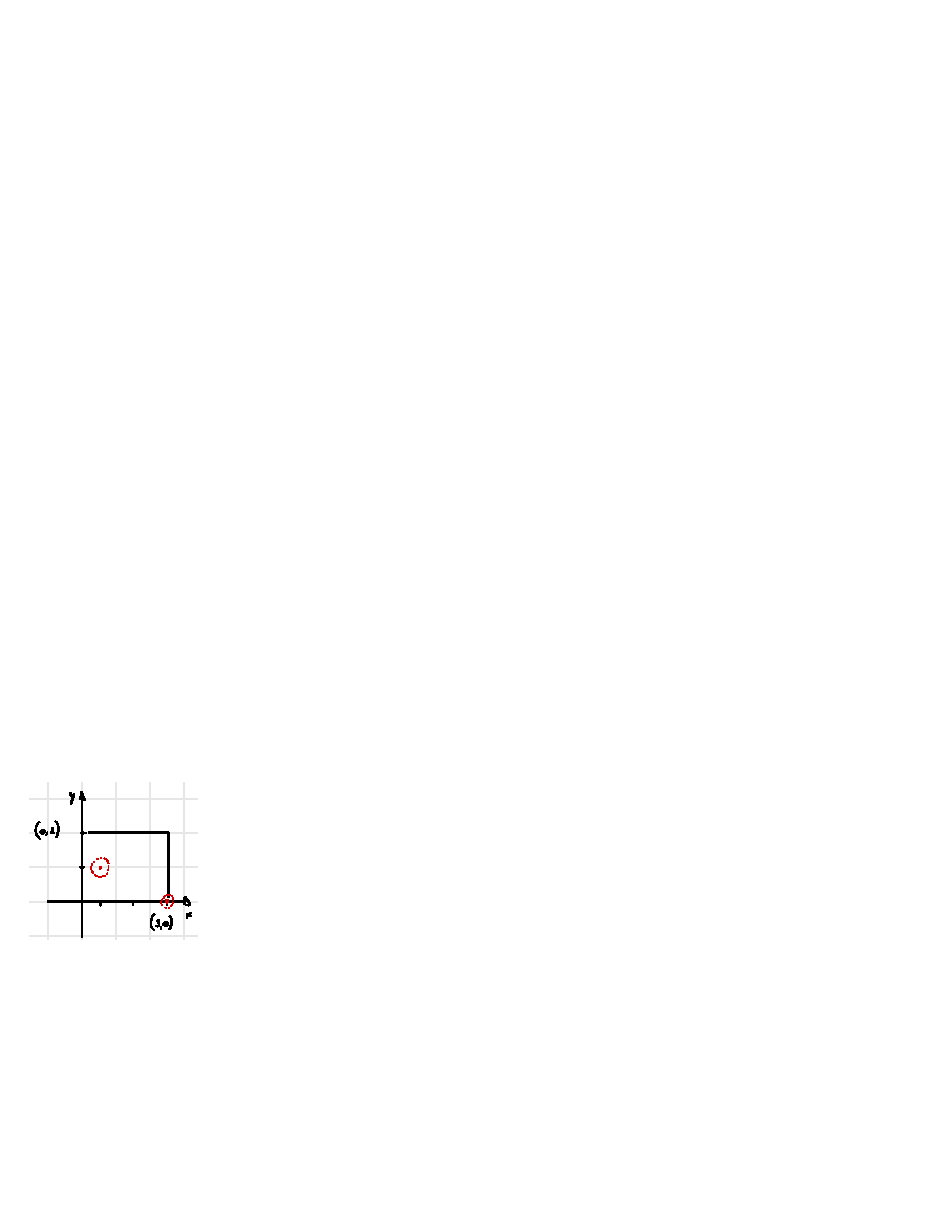
\includegraphics[width=0.5\textwidth]{img/esempio_topologia.pdf}
	\end{figure}

	\noindent
	Nella figura si rappresentano i punti di coordinate $\left(1,1\right)$ e $\left(3,0\right)$.\newline
	
	\noindent
	\textcolor{Green4}{\textbf{\underline{Risposta - Domanda 1}}}\newline
	
	\noindent
	$U$ è intorno di $v = \left(1,1\right)$ perché $B_{\frac{1}{2}}\left(v\right) \subseteq U$. La funzione $B$ ha come pedice $\frac{1}{2}$ poiché questa frazione rappresenta il raggio e infatti è centrata $\left(\frac{1}{2} \cdot 2 = 1\right)$.\newline
	
	\noindent
	\textcolor{Green4}{\textbf{\underline{Risposta - Domanda 2}}}\newline
	
	\noindent
	$U$ \emph{non} è intorno di $v = \left(3,0\right)$ poiché sicuramente almeno un punto è fuori da $U$.
	
	\newpage
	
	\noindent\fcolorbox{Red3}{white}{%
		\parbox{\textwidth}{%
			\textcolor{Red3}{\textbf{\underline{Definizione}}}\newline
			
			\noindent
			Dato un insieme $A$ si definiscono:
			
			\begin{itemize}
				\item \textbf{Punto interno}: tutti i punti dell'intorno sono dentro $A$.
				 
				\item \textbf{Punto di frontiera}: alcuni punti sono dentro e altri fuori.
				
				\item \textbf{Punto esterno}: tutti i punti sono esterni ad $A$.
			\end{itemize}
		}%
	}

	\begin{figure}[!htp]
		\centering
		\includegraphics[width=0.7\textwidth]{img/punti.pdf}
		\caption{Punto esterno, interno e di frontiera.}
	\end{figure}

	\newpage
	
	\section{Lezione 08}
	
	\subsection{Insiemi}
	
	Un \textbf{insieme} $A \subseteq \mathbb{R}^{n}$ (sottoinsieme di $\mathbb{R}^{n}$) si dice \textcolor{Red3}{\textbf{\underline{aperto}}} se è intorno di ogni punto, ovvero:
	
	\begin{equation*}
		\forall x_{0} \in A \hspace{1em} \underbrace{\exists r > 0}_{\text{esiste una palla}} \text{ tale che } B_{r}\left(x_{0}\right)\subseteq A
	\end{equation*}

	\noindent
	Si veda l'esercizio nelle pagine successive per capire meglio.\newline
	
	\noindent
	Un \textbf{insieme} $A \subseteq \mathbb{R}^{n}$ (sottoinsieme di $\mathbb{R}^{n}$) si dice \textcolor{Red3}{\textbf{\underline{chiuso}}} se il suo complementare $A^{c}$ è aperto.

	\noindent
	\textbf{\underline{Nota bene:}} per \emph{complementare} si intende la differenza tra insiemi, in questo caso tra l'insieme $\mathbb{R}^{n}$ e l'insieme $A$, formalmente $\mathbb{R}^{n} \setminus A$.\newline
	
	\noindent
	Esiste anche una famiglia di \textcolor{Red3}{\textbf{\underline{insiemi speciali}}} chiamati cosi poiché sono sia chiusi che aperti: $\mathbb{R}^{n}, \emptyset$.\newline
	
	\noindent
	\textcolor{Red3}{\textbf{\underline{Notazioni}}}
	
	\noindent
	\begin{itemize}
		\item $\mathring{A}$ si intende \dquotes{interno ad $A$}, cioè l'\textbf{insieme} di tutti i \textbf{punti interni} ad $A$ (notazione alternativa $\mathrm{int}\left(A\right)$);
		
		\item $\partial A$ si intende \dquotes{frontiera di $A$}, cioè l'\textbf{insieme} di tutti i \textbf{punti di frontiera} di $A$;
		
		\item $\bar{A}$ si intende \dquotes{chiusura di $A$}, cioè l'\textbf{insieme di tutti i punti} di $A$ uniti alla frontiera. Quindi, il \textbf{più piccolo sottoinsieme} di $\mathbb{R}^{n}$ che contiene $A$, formalmente: $A \cup \partial A$;
		
		\item $\mathrm{est}\left(A\right)$ si intende l'insieme dei \textbf{punti esterni} ad $A$.
	\end{itemize}

	\newpage
	
	\subsubsection[Esempio 1]{\textcolor{Green4}{Esempio 1}}
	
	Dato l'insieme:
	
	\begin{equation*}
		A = \left\{x \in \mathbb{R}^{n} : 2 < \Big||x-x_{0}|\Big| \le 3\right\} \hspace{2em} \text{con } x_{0} \in \mathbb{R}^{n}
	\end{equation*}

	\noindent
	Si vuole ottenere $\mathring{A}, \partial A, \bar{A}$, ovvero l'insieme dei punti interni, di frontiera e di chiusura. La rappresentazione è la seguente:
	
	\begin{figure}[!htp]
		\centering
		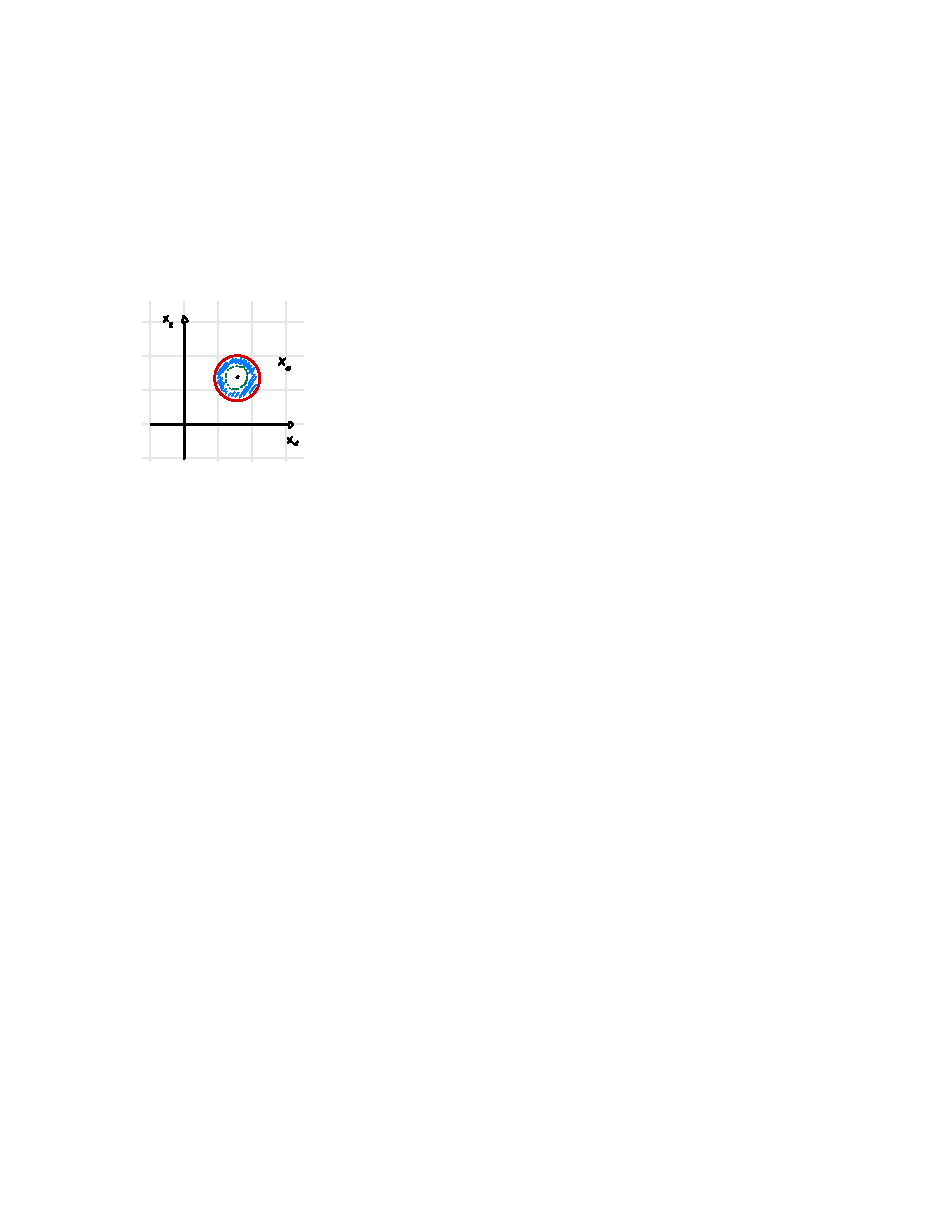
\includegraphics[width=0.5\textwidth]{img/ex1_insiemi.pdf}
		\caption{Grafico dell'insieme $A$ con $n = 2$ (bidimensionale).}
	\end{figure}

	\noindent
	Con raggio uguale a $2$ (linea tratteggiata verde, la più interna), la linea viene disegnata tratteggiata perché non appartiene ad $A$ (si guardi il dominio per capire perché il $2$ non è accettato!).\newline
	
	\noindent
	Al contrario, con raggio $3$ (linea continua rosso, la più esterna), la linea viene disegnata in modo continuo poiché appartiene ad $A$ (nel dominio c'è il minore uguale che ci consente di affermare che il $3$ può appartenere ad $A$).\newline
	
	\noindent
	Infine, con il colore blu si identificano i punti che sono interni ad $A$.\newline
	
	\noindent
	Si definiscono gli insiemi richiesti:
	
	\begin{itemize}
		\item I punti \textbf{interni} ad $A$ vengono definiti nel seguente modo:
		\begin{equation*}
			\mathring{A} = \left\{x \in \mathbb{R}^{n} : 2 < \Big||x-x_{0}|\Big| < 3\right\}
		\end{equation*}
		
		\item I punti di \textbf{frontiera} ad $A$ vengono definiti nel seguente modo:
		\begin{equation*}
			\partial A = \left\{x \in \mathbb{R}^{n} : \Big||x-x_{0}|\Big| = 2 \hspace{0.5em} \lor \hspace{0.5em} \Big||x-x_{0}|\Big| = 3 \right\}
		\end{equation*}
		
		\item I punti di \textbf{chiusura} ad $A$ vengono definiti nel seguente modo:
		\begin{equation*}
			\bar{A} = \left\{x \in \mathbb{R}^{n} : 2 \le \Big||x-x_{0}|\Big| \le 3\right\}
		\end{equation*}
	\end{itemize}

	\noindent
	Dalla definizione degli insiemi, si deduce che l'\textbf{insieme non è né aperto né chiuso}. Infatti, un \textcolor{Red3}{\textbf{\underline{insieme}}} si dice:
	
	\begin{itemize}[label=-]
		\item \textcolor{Red3}{\textbf{\underline{Aperto}}} se e solo se coincide con il suo interno;
		
		\item \textcolor{Red3}{\textbf{\underline{Chiuso}}} se e solo se coincide con la sua chiusura;
	\end{itemize}

	\newpage
	
	\subsubsection[Esempio 2]{\textcolor{Green4}{Esempio 2}}
	
	Dato l'insieme $B$:
	
	\begin{equation*}
		B = \left(B_{2}\left(\overrightarrow{0}\right) \setminus \left(\left[-1,1\right] \times \left\{0\right\}\right)\right) \cup \left(\left(-1,1\right) \times \left\{3\right\}\right)
	\end{equation*}

	\noindent
	Si esamina la sua definizione e si ottengono le seguenti informazioni:
	
	\begin{itemize}[label=-]
		\item $B_{2}\left(\overrightarrow{0}\right)$, rappresenta la palla di raggio $2$ centrata nell'origine. Infatti:
		\begin{equation*}
			\left\{\underbrace{\left(x,y\right)}_{\overrightarrow{P}} \in \mathbb{R}^{2} : \mathrm{d}\left(\overrightarrow{P}, \overrightarrow{0}\right) < 2\right\}
		\end{equation*}
		In cui la definizione $\mathrm{d}\left(\overrightarrow{P}, \overrightarrow{0}\right) < 2$ indica i punti della palla che hanno distanza minore di $2$.
		
		\item $\setminus \left(\left[-1,1\right] \times \left\{0\right\}\right)$, rappresenta la sottrazione di questo intervallo, il quale è definito come:
		\begin{equation*}
			\left\{\left(x,y\right) \in \mathbb{R}^{2} : -1 \le x \le 1, y = 0\right\}
		\end{equation*}
	
		\item $\cup \left(\left(-1,1\right) \times \left\{3\right\}\right)$, rappresenta l'unione con questo intervallo, quest'ultimo definito come:
		\begin{equation*}
			\left\{\left(x,y\right) \in \mathbb{R}^{2} : -1 < x < 1, y = 3\right\}
		\end{equation*}
	\end{itemize}

	\noindent
	La rappresentazione grafica:
	
	\begin{figure}[!htp]
		\centering
		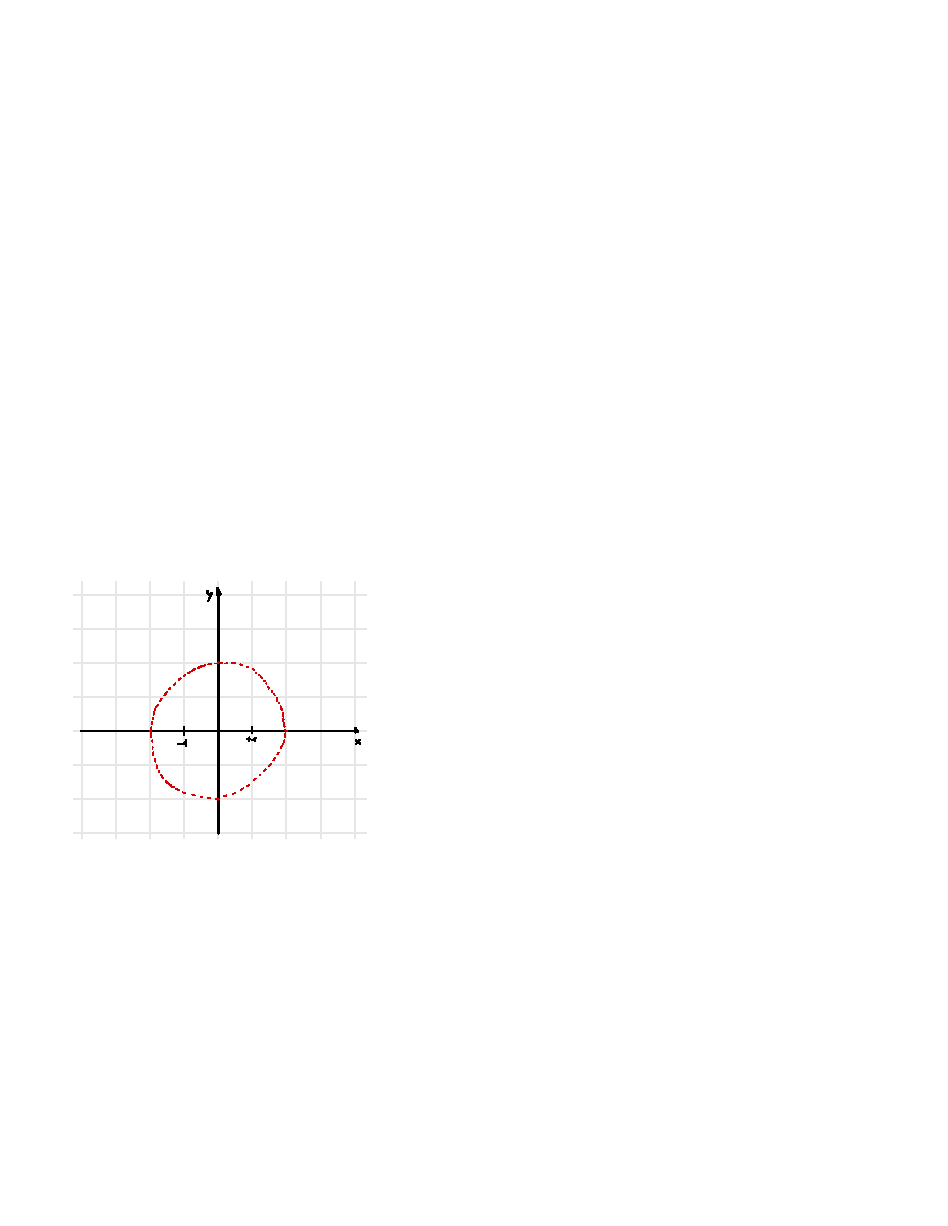
\includegraphics[width=0.5\textwidth]{img/ex2_insiemi.pdf}
		\caption{Rappresentazione grafica $B_{2}\left(\overrightarrow{0}\right)$.}
		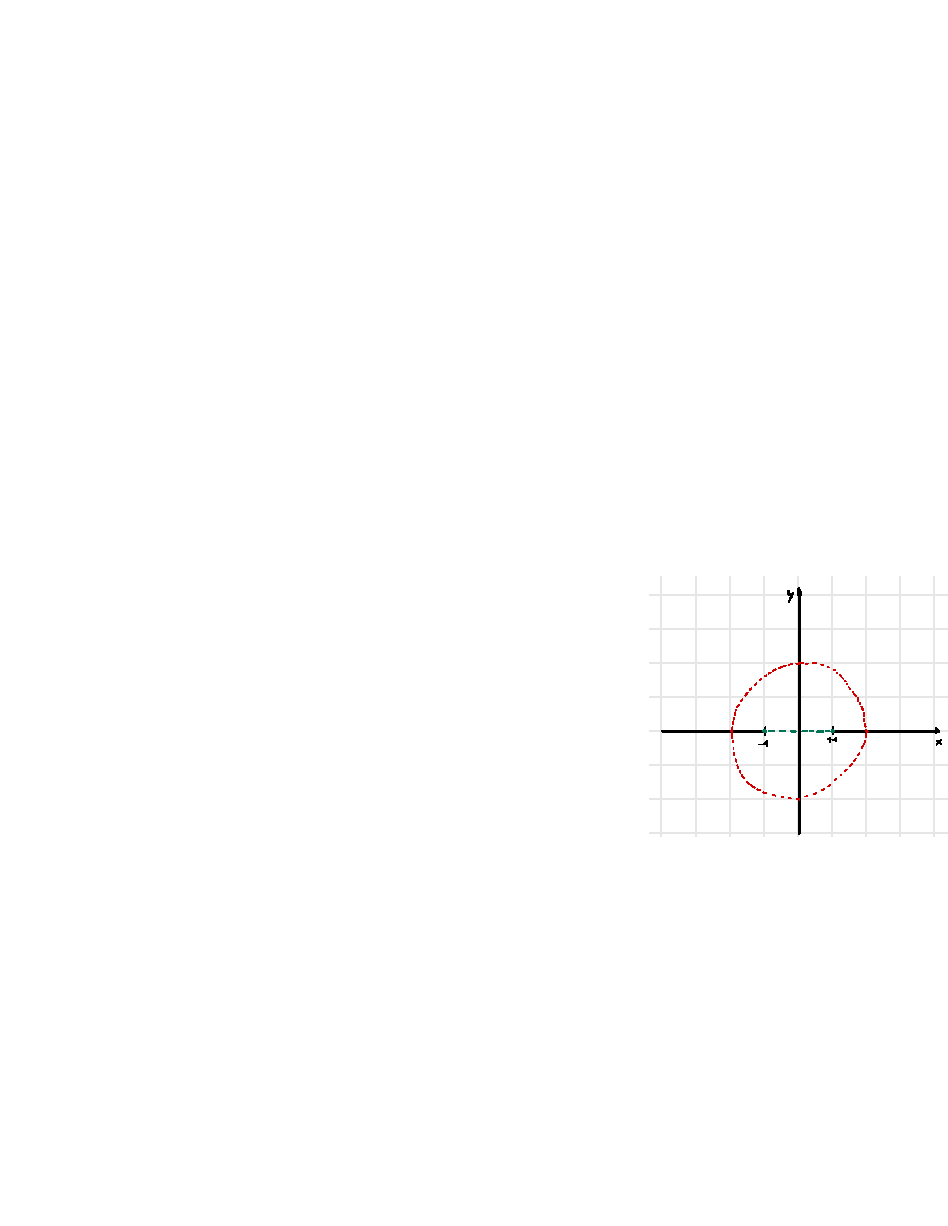
\includegraphics[width=0.5\textwidth]{img/ex2-2_insiemi.pdf}
		\caption{Sottrazione dell'intervallo, estremi compresi $\left[-1,1\right] \times \left\{0\right\}$.}
		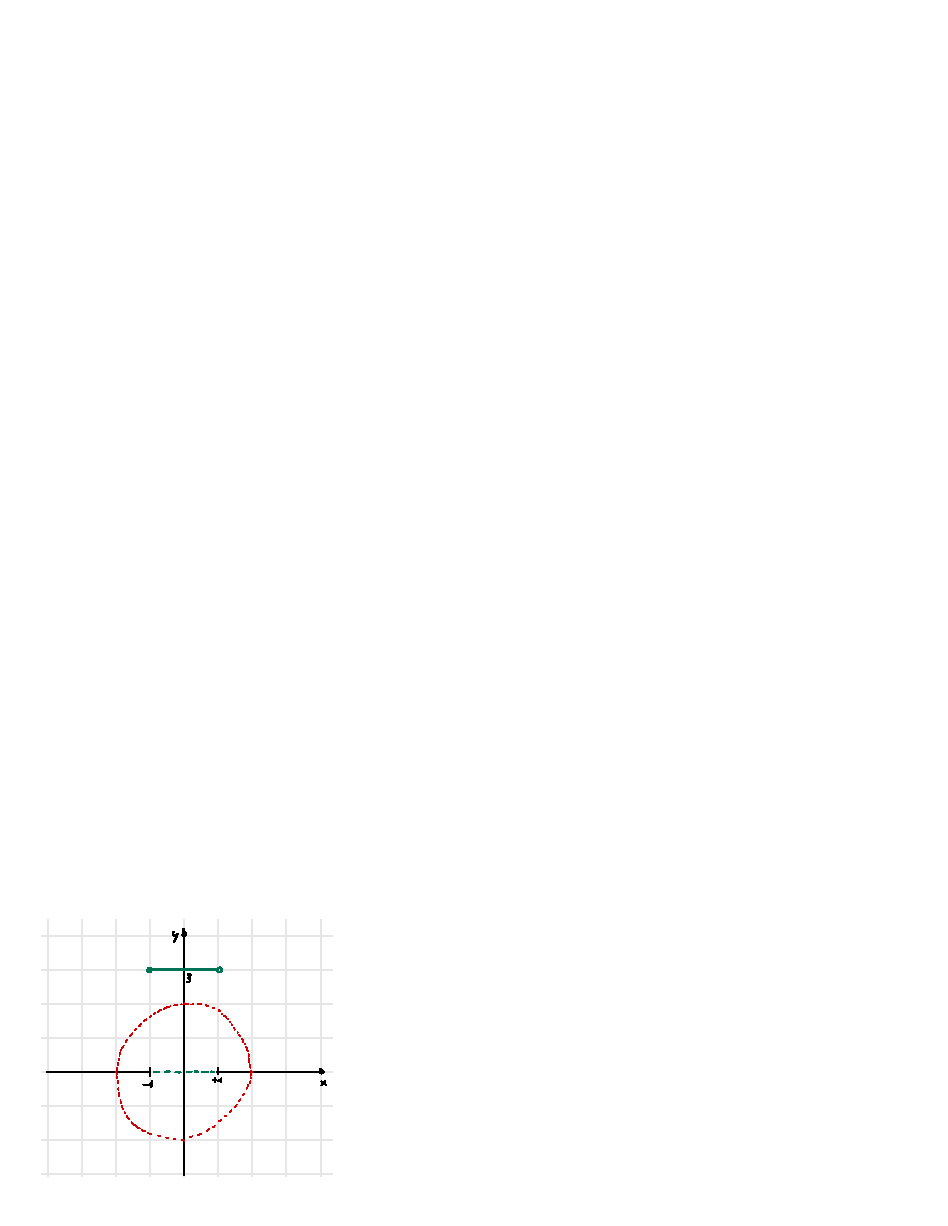
\includegraphics[width=0.5\textwidth]{img/ex2-3_insiemi.pdf}
		\caption{Unione con l'intervallo, estremi esclusi $\left(-1,1\right) \times \left\{3\right\}$.}
	\end{figure}

	\newpage

	\noindent
	Quindi, i punti interni sono:
	
	\begin{equation*}
		\mathring{B} = B_{2}\left(\overrightarrow{0}\right) \setminus \left(\left[-1,1\right] \times \left\{0\right\}\right)
	\end{equation*}

	\noindent
	Invece, i punti di frontiera sono definiti dal seguente insieme:
	
	\begin{equation*}
		\partial B = \left\{\left(x,y\right) \in \mathbb{R}^{2} : \sqrt{x^{2} + y^{2}} = 2\right\} \cup \left(\left[-1,1\right] \times \left\{0\right\}\right) \cup \left(\left[-1,1\right] \times \left\{3\right\}\right)
	\end{equation*}
	
	\noindent
	In cui la definizione $\left\{\left(x,y\right) \in \mathbb{R}^{2} : \sqrt{x^{2} + y^{2}} = 2\right\}$ identifica i punti sulla circonferenza.
	
	\newpage
	
	\subsubsection{Insieme limitato e punto di accumulazione}
	
	\noindent
	Un insieme $A \subseteq \mathbb{R}^{n}$ (sottoinsieme dell'insieme $\mathbb{R}^{n}$) è \textcolor{Red3}{\textbf{\underline{limitato}}} se $\exists r > 0$ tale che $A \subseteq B_{r}\left(\overrightarrow{0}\right)$. In altre parole, se $\exists r > 0$ tale che $\Big||x|\Big| < r$ per ogni $x \in A$. Visivamente:
	
	\begin{figure}[!htp]
		\centering
		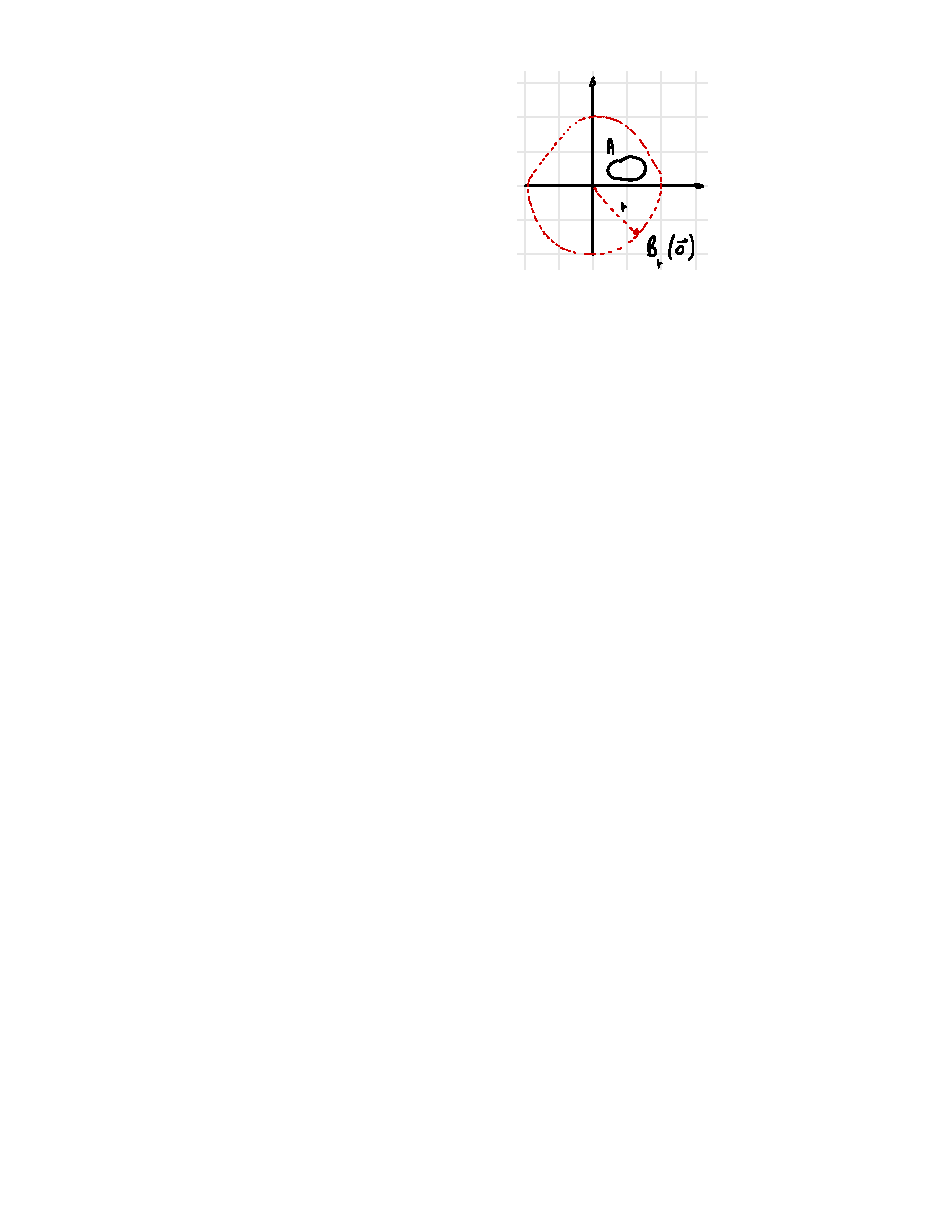
\includegraphics[width=0.43\textwidth]{img/insiemi_limitati.pdf}
		\caption{Definizione di insieme limitato.}
	\end{figure}

	\noindent
	Dato un insieme $A \subseteq \mathbb{R}^{n}$ si dice che $x_{0}$ è \textcolor{Red3}{\textbf{\underline{punto di accumulazione}}} per $A$ se per ogni $r > 0$:
	
	\begin{equation*}
		B_{r}\left(x_{0}\right) \cap \left(A \setminus \left\{x_{0}\right\}\right) \ne \emptyset
	\end{equation*}

	\subsubsection[Esempio 3]{\textcolor{Green4}{Esempio 3}}
	
	Dato l'insieme $A$:
	
	\begin{equation*}
		A = \left(0,1\right) \times \left[0,1\right] \times \left[0,1\right) \cup \left\{\left(0,0,2\right)\right\} \hspace{2em} \text{con } A \subseteq \mathbb{R}^{3}
	\end{equation*}

	\noindent
	Il punto $\left(0,0,2\right)$ è il punto isolato di $A$. Infatti, la rappresentazione grafica:
	
	\begin{figure}[!htp]
		\centering
		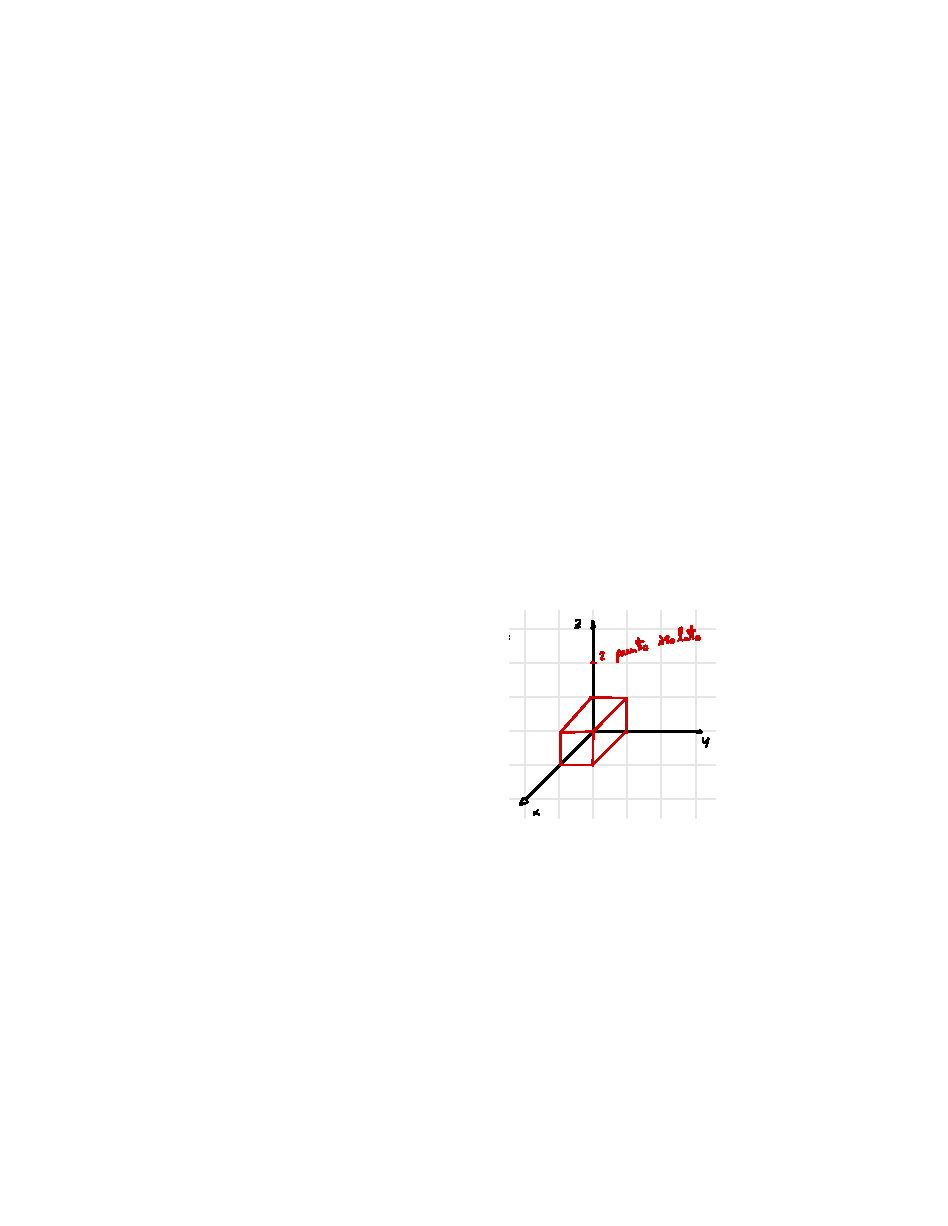
\includegraphics[width=0.43\textwidth]{img/esempio_insieme.pdf}
		\caption{La rappresentazione grafica con $n = 3$.}
	\end{figure}

	\noindent
	L'insieme dei punti di accumulazione di $A$ viene indicata con $A' = \left[0,1\right]^{3}$.
	
	\subsection{Funzioni a più variabili}
	
	Le \textcolor{Red3}{\textbf{\underline{funzioni a più variabili}}} sono funzioni da $\mathbb{R}^{n}$ a $\mathbb{R}$, che prendono un vettore e lo trasformano in numero reale:
	
	\begin{equation*}
		\begin{array}{lcll}
			f:	&	D \subseteq \mathbb{R}^{n}	& \longrightarrow & \mathbb{R} \\
				&	x							& \longmapsto	  & f\left(x\right)
		\end{array}
	\end{equation*}

	\noindent
	Dove $x$ è formato da $\left(x_{1}, ..., x_{n}\right)$. Quindi, la funzione viene definita, ovvero il grafico viene definito nel seguente modo:
	
	\begin{equation}\label{funzioni a più variabili}
		\Gamma\left(f\right) = \left\{\left(x, f\left(x\right)\right) \in \mathbb{R}^{n+1} : x \in D\right\}
	\end{equation}

	\noindent
	\textcolor{Green4}{\textbf{Per esempio}}, si definisce una funzione:
	
	\begin{equation*}
		\begin{array}{llll}
			f:	&	\mathbb{R}^{2}	& \longrightarrow & \mathbb{R} \\
				&	\left(x,y\right)& \longmapsto	  & 1
		\end{array}
	\end{equation*}

	\noindent
	Quindi $z$ sarà sempre uguale a $1$.
	
	\newpage
	
	\subsection{Esercizio d'\textcolor{Red3}{esame}}
	
	\textcolor{Red3}{\textbf{\emph{\underline{Esercizio}}}}\newline
	
	\noindent
	Data la funzione $f\left(x,y\right) = \sqrt{9 - x^{2} - y^{2}}$ si chiede di rispondere alle seguenti domande:
	
	\begin{enumerate}
		\item Qual è il dominio della funzione?
		\item Si rappresenti la funzione in un grafico.
	\end{enumerate}

	\noindent
	\textcolor{Green4}{\textbf{\emph{\underline{Risoluzione}}}}\newline
	
	\noindent
	Il \textbf{dominio} è il seguente:
	
	\begin{equation*}
		D_{f} = \left\{\left(x,y\right) \in \mathbb{R}^{2} : 9 - x^{2} - y^{2} \ge 0\right\}
	\end{equation*}

	\noindent
	Poiché per rimanere nell'insieme dei reali, la radice quadrata non deve essere negativa, altrimenti l'insieme sarebbe quello dei complessi. Sistemando la disuguaglianza, il dominio diventa:

	\begin{equation*}
		D_{f} = \left\{\left(x,y\right) \in \mathbb{R}^{2} : 9 - x^{2} - y^{2} \ge 0\right\} \longrightarrow
		D_{f} = \left\{\left(x,y\right) \in \mathbb{R}^{2} : x^{2} + y^{2} \le 9\right\}
	\end{equation*}

	\noindent
	Il grafico si rappresenta ed è il seguente:
	
	\begin{figure}[!htp]
		\centering
		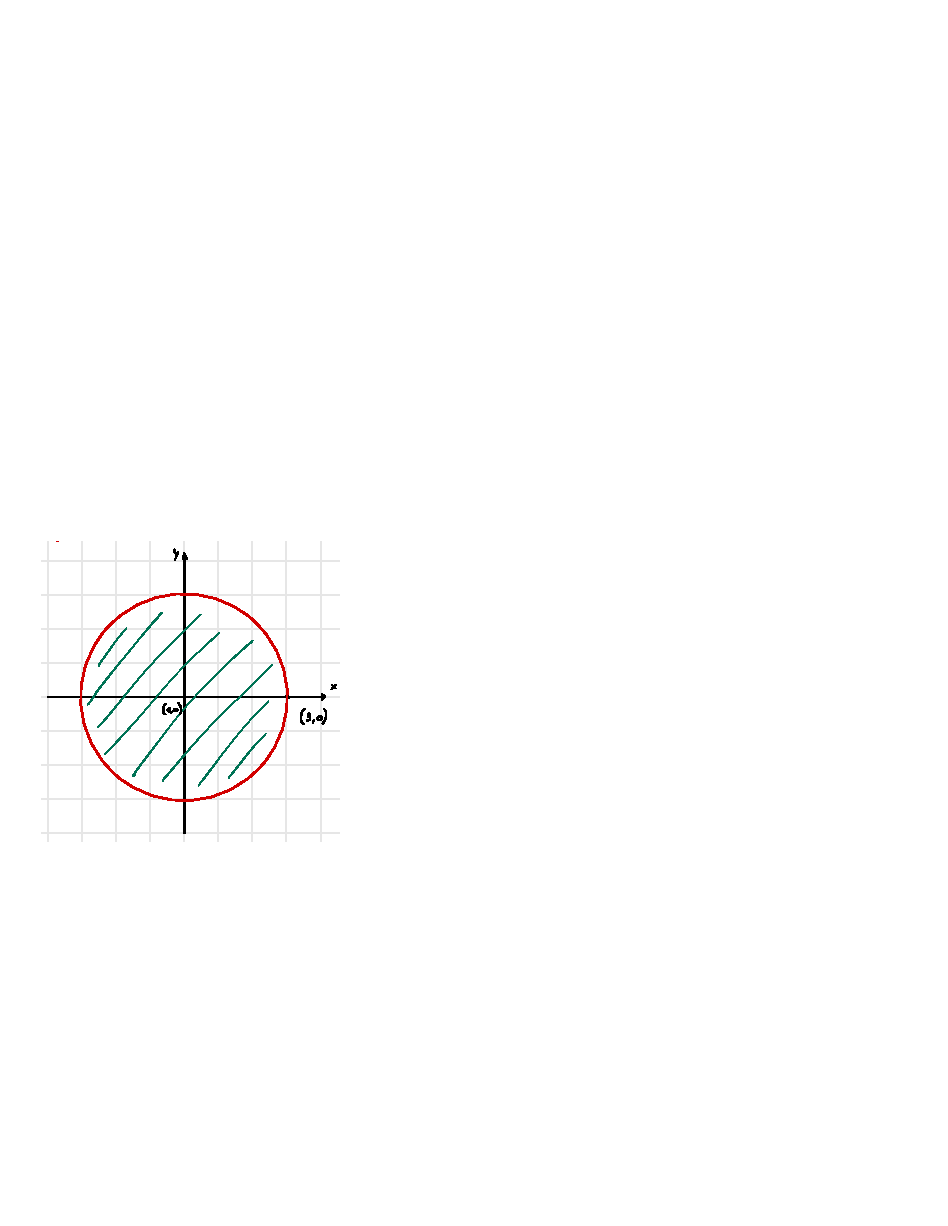
\includegraphics[width=0.5\textwidth]{img/grafico_esame1.pdf}
		\caption{Grafico della funzione.}
	\end{figure}

	\noindent
	Il dominio è dentro al cerchio ed è definito come:
	
	\begin{equation*}
		\Gamma\left(f\right) = \left\{\left(x,y,z\right) \in \mathbb{R}^{3} : z = \sqrt{9 - x^{2} - y^{2}}, \left(x,y\right) \in D_{f}\right\}
	\end{equation*}

	\noindent
	Si osserva che la variabile $z$ deve essere necessariamente maggiore uguale a zero $\left(z \ge 0\right)$ poiché altrimenti il valore non sarebbe nell'insieme dei reali. Inoltre si ha l'equazione:
	
	\begin{equation*}
		z^{2} = 9 - x^{2} + y^{2} \longrightarrow x^{2} + y^{2} + z^{2} = 9
	\end{equation*}

	\noindent
	L'equazione rappresenta la norma euclidea al quadrato: $\Big||\left(x,y,z\right)|\Big|^{2}$, quindi il grafico con $n = 3$ è il seguente:
	
	\begin{figure}[!htp]
		\centering
		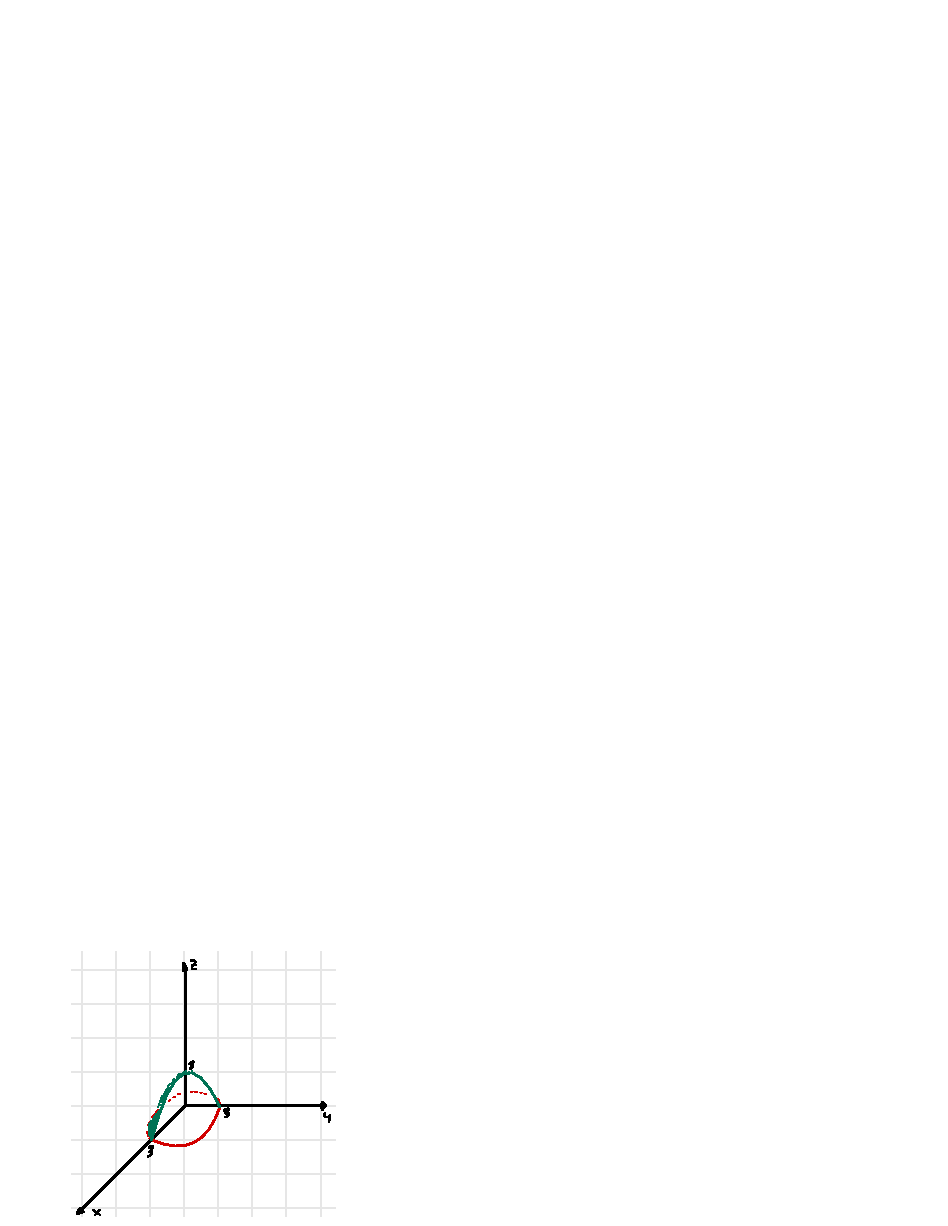
\includegraphics[width=0.5\textwidth]{img/grafico2_esame1.pdf}
	\end{figure}

	\noindent
	\textbf{\underline{Attenzione!}} L'esame continua nel prossimo capitolo con l'introduzione di un nuovo argomento.

	\newpage
	
	\subsection{Insiemi (curve) di livello}
	
	Gli insiemi, o curve, di livello sono definiti come:
	
	\begin{equation*}
		L_{k}\left(f\right) = \left\{x \in D : f\left(x\right) = k\right\}
	\end{equation*}

	\noindent
	Con $k$ che indica il livello da rappresentare.
	
	\begin{figure}[!htp]
		\centering
		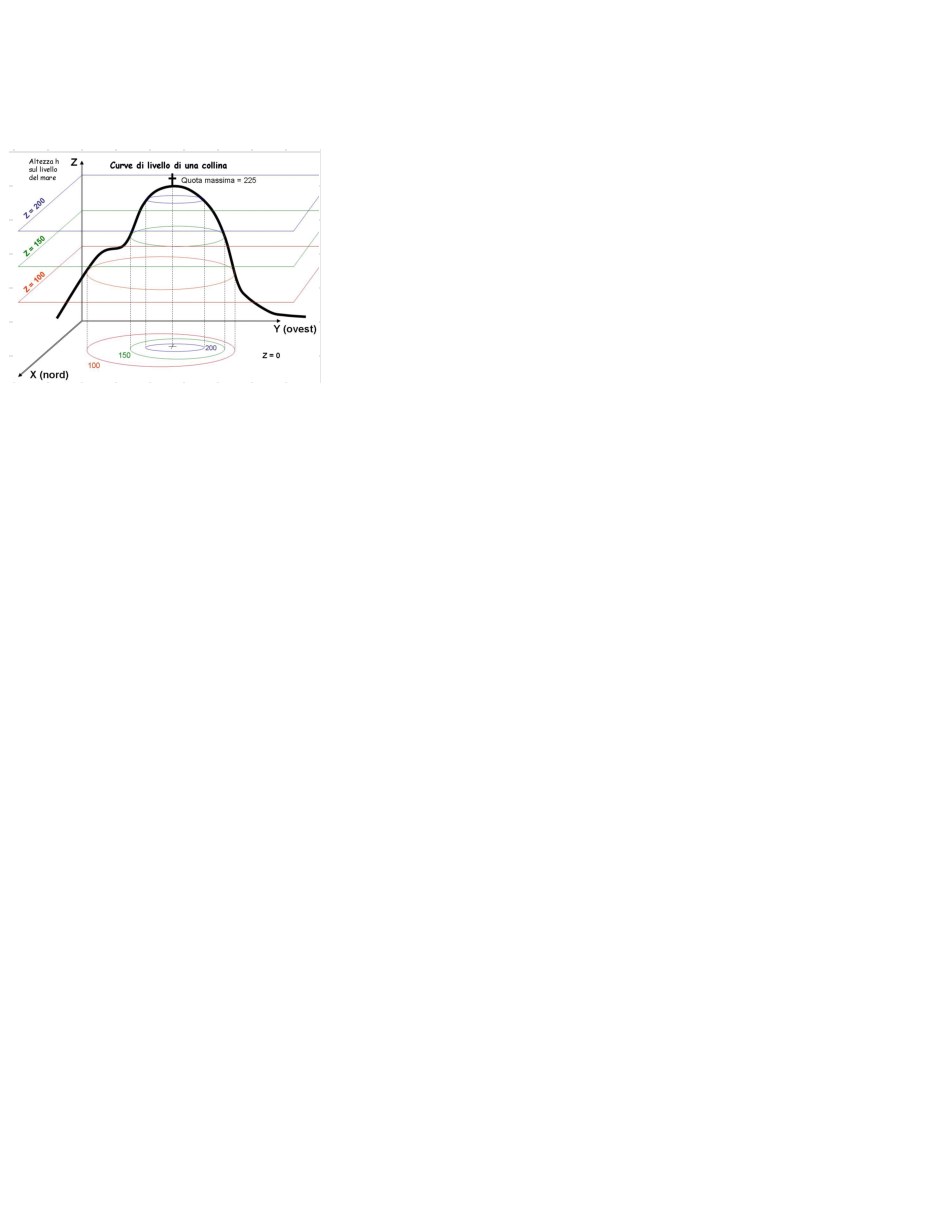
\includegraphics[width=0.5\textwidth]{img/insiemi_di_livello.pdf}
		\caption{Esempio di curve di livello.}
	\end{figure}

	\noindent
	\textcolor{Green4}{\textbf{\underline{Per esempio}}}, se $n = 2$, allora la funzione $L_{k}\left(f\right)$ è l'intersezione tra il grafico di $f$ e il piano $z = k$, proiettata sul piano $xy$.\newline
	
	\noindent
	\textcolor{Red3}{\textbf{\underline{Continuo dell'esame precedente}}}\newline
	
	\noindent
	Ricordando che la funzione dell'esame era:
	
	\begin{equation*}
		f\left(x,y\right) = \sqrt{9 - x^{2} - y^{2}}
	\end{equation*}

	\noindent
	Le sue curve di livello sono $\sqrt{9 - x^{2} - y^{2}} = k$ con diversi valori di $k$:
	
	\begin{itemize}
		\item $k \ge 0$ i passaggi sono i seguenti:
		\begin{equation*}
			\begin{array}{lrll}
								& \sqrt{9 - x^{2} - y^{2}} 	& = & k \\
				\longrightarrow	& 9 - x^{2} - y^{2}			& = & k^{2} \\
				\longrightarrow	& x^{2} + y^{2}				& = & 9 - k^{2}
			\end{array}
		\end{equation*}
		La quale rappresenta la circonferenza con raggio $\sqrt{9 - k^{2}}$ con $k \le 3$ e centro in $\left(0,0\right)$.
		
		\item $k < 0$ è un insieme vuoto, formalmente: $L_{k}\left(f\right) = \emptyset$.
	\end{itemize}

	\newpage
	
	\subsection{Esercizio d'\textcolor{Red3}{esame}}
	
	\textcolor{Red3}{\textbf{\underline{\emph{Esercizio}}}}\newline
	
	\noindent
	Data la funzione $f\left(x,y\right) = \sqrt{x + y + 1} - \log\left(x^{2} - y\right)$ e la funzione $g\left(x,y\right) = \sqrt{\log\left(1-3xy\right)}$.
	
	\noindent
	Si vuole:
	
	\begin{enumerate}
		\item Il dominio delle funzioni (all'esame è possibile anche richiedere punti di frontiera, interni, ecc.);
		
		\item Rappresentare graficamente le due funzioni;
		
		\item Curve di livello con grafico.
	\end{enumerate}

	\noindent
	\textcolor{Green4}{\textbf{\underline{\emph{Risoluzione}}}}\newline
	
	\noindent
	Il \textbf{dominio} della funzione $f$ è la seguente:
	
	\begin{equation*}
		D_{f} = \left\{x,y \in \mathbb{R}^{2} : \hspace{1em} x+y+1 \ge 0, \hspace{1em} x^{2}-y > 0\right\}
	\end{equation*}

	\noindent
	Il \textbf{grafico} della disuguaglianza $x+y+1 \ge 0$:
	
	\begin{figure}[!htp]
		\centering
		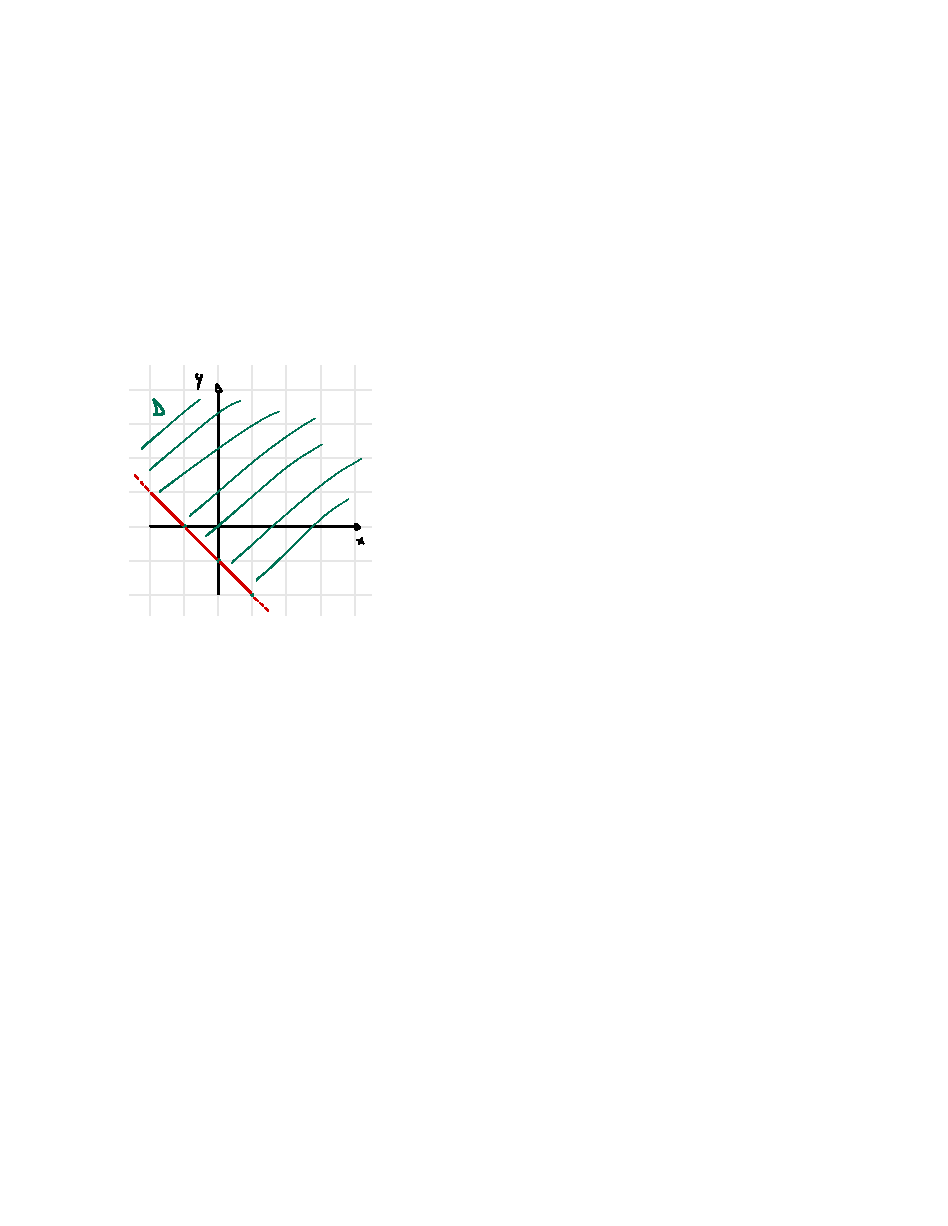
\includegraphics[width=0.5\textwidth]{img/ex1_esame.pdf}
	\end{figure}

	\noindent
	La rappresentazione grafica è stata creata grazie alla classica tabella per rappresentare i punti. Per esempio, si assegna ad $x$ il valore $0$, a questo punto si cerca di calcolare la $y$ per capire quanto vale (in questo caso $-1$). E così via. Bastano anche tre punti per rappresentare la funzione, per esempio con $x = 0, x = 1, x = -1$ si hanno rispettivamente i valori $y = -1, y = -2, y = 0$.
	
	Per capire dov'è il dominio (parte in verde disegnata) si utilizza un \textbf{punto di test}. Per esempio, prendendo le coordinate dell'origine $\left(0,0\right)$, esso verifica la condizione? Ovvero, sostituendo i due valori nella disuguaglianza, quest'ultima risulta vera? Andando a sostituire:
	
	\begin{equation*}
		x+y+1 \ge 0 \xrightarrow{\text{sostituendo il punto di test}} 0 + 0 + 1 \ge 0 \longrightarrow 1 \ge 0 \:\: \textcolor{Green4}{\text{Verificato \checkmark}}
	\end{equation*}

	\newpage
	
	\noindent
	Il \textbf{grafico} della disuguaglianza $x^{2} - y > 0$:
	
	\begin{figure}[!htp]
		\centering
		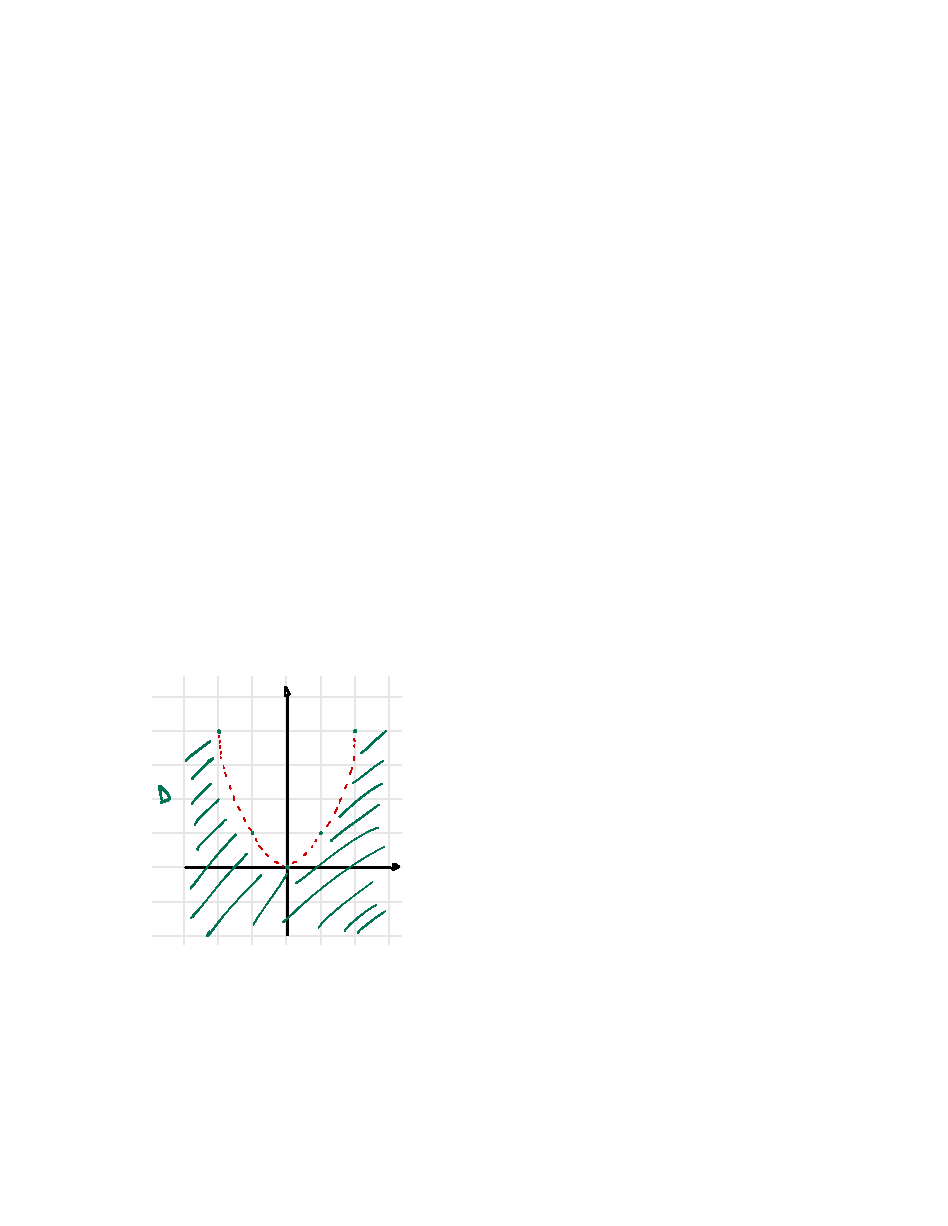
\includegraphics[width=0.5\textwidth]{img/ex1_esame2.pdf}
	\end{figure}

	\noindent
	La rappresentazione grafica viene effettuata nello stesso modo della figura precedente, quindi con i valori di $x = 0, x = 1, x = 2, x = -1, x = -2$, si hanno i valori di $y = 0, y = 1, y = 4, y = 1, y = 4$.
	
	Il dominio viene preso in considerazione sotto la parabola poiché prendendo come \textbf{punto di test} le coordinate $\left(1,0\right)$:
	
	\begin{equation*}
		x^{2} - y > 0 \xrightarrow{\text{sostituendo il punto di test}} 1^{2} - 0 > 0 \:\: \textcolor{Green4}{\text{Verificato \checkmark}}
	\end{equation*}

	\noindent
	L'\textbf{intersezione} delle due disuguaglianze, ovvero il dominio $D_{f}$ si rappresenta con il seguente grafico:
	
	\begin{figure}[!htp]
		\centering
		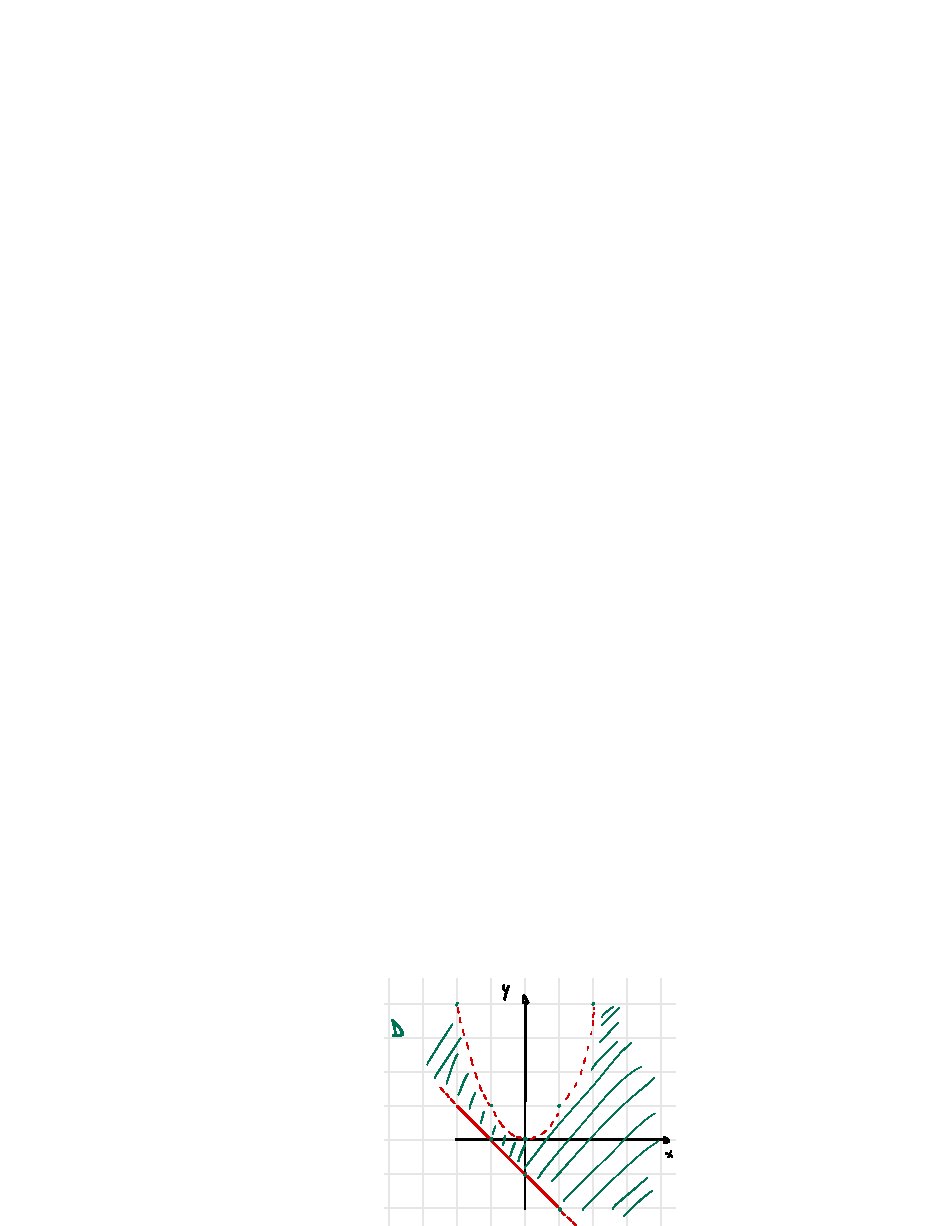
\includegraphics[width=0.5\textwidth]{img/ex1_esame3.pdf}
	\end{figure}

	\newpage
	
	\section{Lezione 09}
	
	\subsection{Come rappresentare una ellisse e iperbole traslata}
	
	Data la funzione di una ellisse iperbole:
	
	\begin{equation*}
		f\left(x,y\right) = \sqrt{11 - 4x^{2} - 9y^{2} + 16x - 18y}
	\end{equation*}
	
	Si calcola:
	
	\begin{itemize}
		\item Rappresentare graficamente il dominio di $f$;
		\item Tracciare la curva di livello $L_{4}\left(f\right)$
	\end{itemize}

	\noindent
	\textcolor{Green4}{\textbf{\underline{\emph{Risoluzione punto 1}}}}\newline

	\noindent
	Il \textbf{dominio} della funzione si traduce in:
	
	\begin{equation*}
		D_{f} = \left\{\left(x,y\right) \in \mathbb{R}^{2} : 11 - 4x^{2} - 9y^{2} + 16x - 18y \ge 0\right\}
	\end{equation*}

	\noindent
	Semplificando la disuguaglianza:
	
	\begin{equation*}
		D_{f} = \left\{\left(x,y\right) \in \mathbb{R}^{2} : 4x^{2} + 9y^{2} - 16x +18y - 11 \le 0\right\}
	\end{equation*}

	\noindent
	La frontiera è il punto in cui la funzione si annulla, dunque:
	
	\begin{equation*}
		4x^{2} + 9y^{2} - 16x +18y - 11 = 0
	\end{equation*}
	
	\noindent
	Per \textbf{ottenere una ellisse traslata}, si applica la \textcolor{Red3}{\textbf{\underline{tecnica}}} del \textcolor{Red3}{\textbf{\underline{completamento del quadrato}}}.\newline
	
	\noindent
	L'\textbf{obbiettivo} è ottenere la forma canonica dell'ellisse traslata:
	
	\begin{equation*}
		\dfrac{\left(x - x_{c}\right)^{2}}{a^{2}} + \dfrac{\left(y - y_{c}\right)^{2}}{b^{2}} = 1
	\end{equation*}

	\noindent
	Ovviamente, nel caso in cui $y_{c}$ e $x_{c}$ sono \textbf{nulli}, allora l'ellisse non è traslata.\newline
	
	\noindent
	Per avere la precedente forma anche nella funzione iniziale, sono necessari alcune manipolazioni. Si raggruppano le $x$ e le $y$ in modo da ottenere $1$ come coefficiente di quadrati:
	
	\begin{equation*}
		\begin{array}{lll}
			\text{Equazione originaria}				 & \longrightarrow & 4x^{2} + 9y^{2} - 16x +18y - 11 = 0 \\
			&& \\
			\text{Raggruppamento}					 & \longrightarrow & 4\left(x^{2} - 4x\right) + 9\left(y^{2} + 2y\right) - 11 = 0 \\
			&& \\
			\text{Secondo raggruppamento}			 & \longrightarrow & 4\left[\left(x - 2\right)^{2} - 4\right] + 9\left[\left(y + 1\right)^{2} - 1\right] - 11 = 0 \\
			&& \\
			\text{Rimozione delle parentesi}		 & \longrightarrow & 4\left(x-2\right)^{2} - 16 + 9\left(y+1\right)^{2} - 9 - 11 = 0 \\
			&& \\
			\text{Si porta a destra il termine noto} & \longrightarrow & 4\left(x-2\right)^{2} + 9\left(y+1\right)^{2} = 36 \\
			&& \\
			\text{Dividendo tutto per il termine noto} & \longrightarrow & \dfrac{\cancel{4} \left(x-2\right)^{2}}{\cancelto{9}{36}} + \dfrac{\cancel{9}\left(y+1\right)^{2}}{\cancelto{4}{36}} = \cancelto{1}{\dfrac{36}{36}}
		\end{array}
	\end{equation*}

	\noindent
	Quindi, il centro ha coordinate pari a $\left(2,-1\right)$ e i semiassi sono $a = 3$ e $b = 2$. Il centro è stato trovato controllando i valori dentro le parentesi, mentre i semiassi basta controllare il denominatore e fare la radice quadrata.\newline
	
	\noindent
	Si rappresenta la funzione in un grafico:
	
	\begin{figure}[!htp]
		\centering
		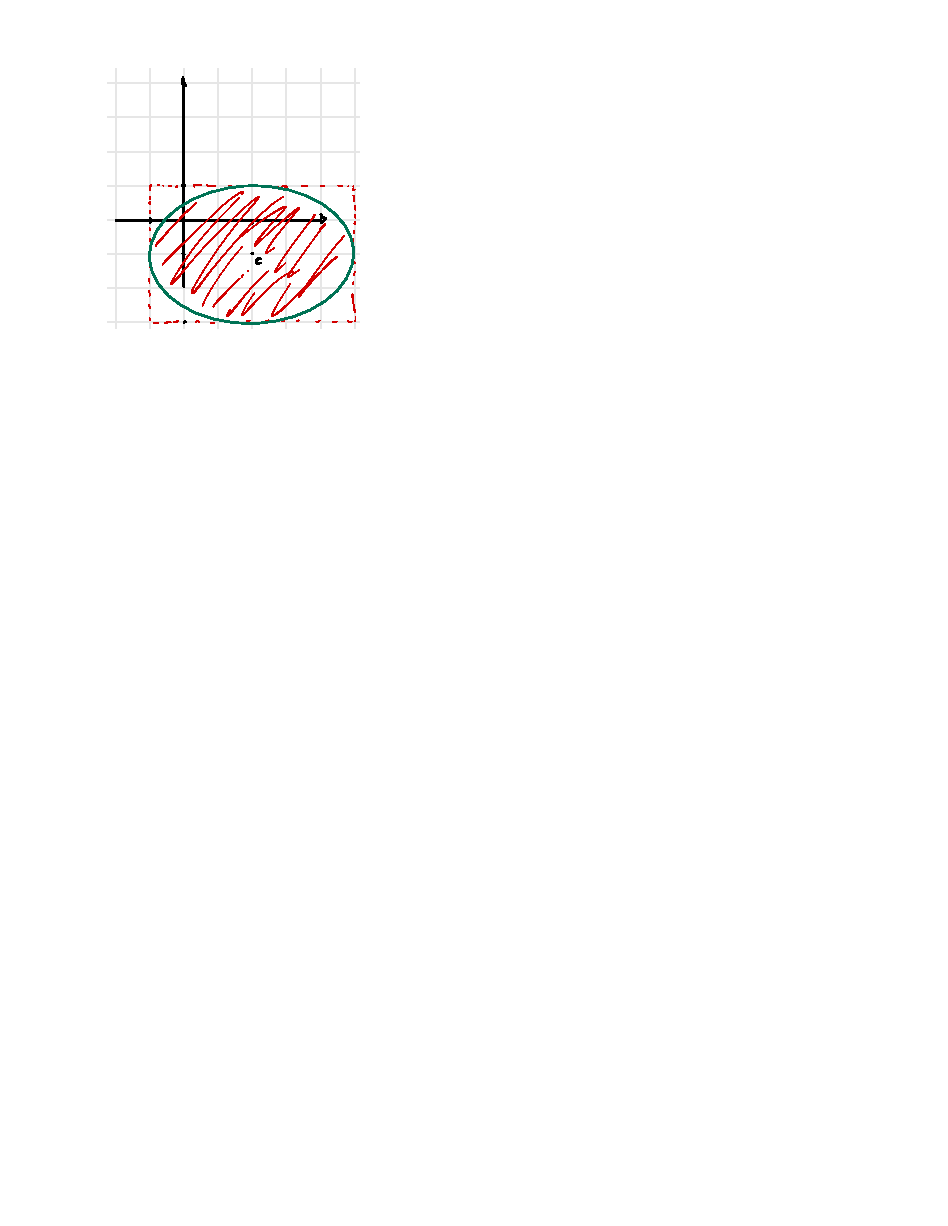
\includegraphics[width=0.5\textwidth]{img/ellisse_iperbole_traslata.pdf}
	\end{figure}

	\noindent
	Il dominio è dentro l'ellisse perché con il punto di test $\left(0,0\right)$, la disuguaglianza viene verificata:
	
	\begin{equation*}
		4x^{2} + 9y^{2} - 16x +18y - 11 \le 0 \xrightarrow{\text{sostituzione punto di test}} 4 \cdot 0^{2} + 9 \cdot 0^{2} - 16 \cdot 0 + 18 \cdot 0 - 11 \le 0 \textcolor{Green4}{\textbf{ \: Verificata \checkmark}}
	\end{equation*}

	\noindent
	\textcolor{Green4}{\textbf{\underline{\emph{Risoluzione punto 2}}}}\newline
	
	\noindent
	La curva di livello si definisce nel seguente modo:
	
	\begin{equation*}
		L_{4}\left(f\right) = \left\{\left(x,y\right) \in \mathbb{R}^{2} : \sqrt{11 - 4x^{2} - 9y^{2} + 16x - 18y} = 4\right\}
	\end{equation*}

	\noindent
	Si studiano i vari casi:
	
	\begin{itemize}[label=-]
		\item $k < 0$, si ha la curva di livello nulla $L_{4}\left(f\right) = \emptyset$;
		
		\item $k = 0$, si ha la circonferenza dell'ellisse;
		
		\item $k > 0$, si ha la curva di livello pari a:
		\begin{gather*}
			\begin{array}{lrll}
				L_{4}\left(f\right):& \sqrt{11 - 4x^{2} - 9y^{2} + 16x - 18y}	& = & 4 \\
				&&& \\
									& 11 - 4x^{2} - 9y^{2} + 16x - 18y			& = & 4^{2} \\
				&&& \\
									& 4x^{2} + 9y^{2} - 16x + 18y + 5			& = & 0
			\end{array}
			\\
			\textbf{applicando la tecnica del completamento del quadrato}\\
			L_{4}\left(f\right): \dfrac{\left(x - 2\right)^{2}}{5} + \dfrac{\left(y + 1\right)^{2}}{\frac{20}{9}} = 1
		\end{gather*}
		Se ne deduce che l'ellisse ha il centro in coordinate $c\left(2,-1\right)$ e semiassi pari ad $a = \sqrt{5}, b = \sqrt{\frac{20}{9}}$.
	\end{itemize}
	
	\newpage
	
	\subsection{Curve sezione}
	
	Le curve sezione sono definite nel seguente modo:
	
	\begin{equation*}
		\begin{cases}
			z = f\left(x,y\right) \\
			x = k
		\end{cases}
	\end{equation*}

	\noindent
	\textcolor{Red3}{\textbf{\underline{Riprendendo l'equazione dell'esercizio precedente}}}\newline
	
	\noindent
	L'equazione con $k = 0$ è $z = \sqrt{11 - 9y^{2} - 18y}$ e di sicuro la $z$ vale $z \ge 0$. Per trovare le curve sezione si costruisce il sistema:
	
	\begin{equation*}
		\begin{cases}
			z \ge 0 \\
			z^{2} = 11 - 9y - 18y
		\end{cases}
		\longrightarrow
		\begin{cases}
			z \ge 0 \\
			9y^{2} + z^{2} + 18y - 11 = 0
		\end{cases}
	\end{equation*}
	
	\noindent
	Applicando la tecnica del completamento del quadrato si ha il seguente svolgimento:
	
	\begin{equation*}
		\begin{array}{rll}
			9y^{2} + z^{2} + 18y - 11 						& = &  0 \\
			&& \\
			9\left[\left(y+1\right)^{2} - 1\right] + z^{2}	& =	& 11 \\
			&& \\
			9\left(y+1\right)^{2} + z^{2}					& = & 20 \\
			&& \\
			\dfrac{\left(y+1\right)^{2}}{\frac{20}{9}} + \dfrac{z^{2}}{20} = 1
		\end{array}
	\end{equation*}

	\newpage
	
	\subsection{Continuità}
	
	Sia $f$ una funzione definita come $D \subseteq \mathbb{R}$ con $x_{0} \in D$. La funzione $f$ si dice \textcolor{Red3}{\textbf{\underline{continua}}} in $x_{0}$ se per ogni intorno $V$ di $f\left(x_{0}\right)$ esiste un intorno $U$ di $x_{0}$ tale per cui:
	
	\begin{equation*}
		f\left(x\right) \in V \hspace{2em} \forall x \in U \cap D
	\end{equation*}

	\noindent
	Dove la $D$ indica il dominio della funzione.\newline
	
	\noindent
	\textcolor{Green4}{\textbf{\emph{\underline{Commento}}}}\newline
	
	\noindent
	Si rappresenta il grafico di una palla continua:
	
	\begin{figure}[!htp]
		\centering
		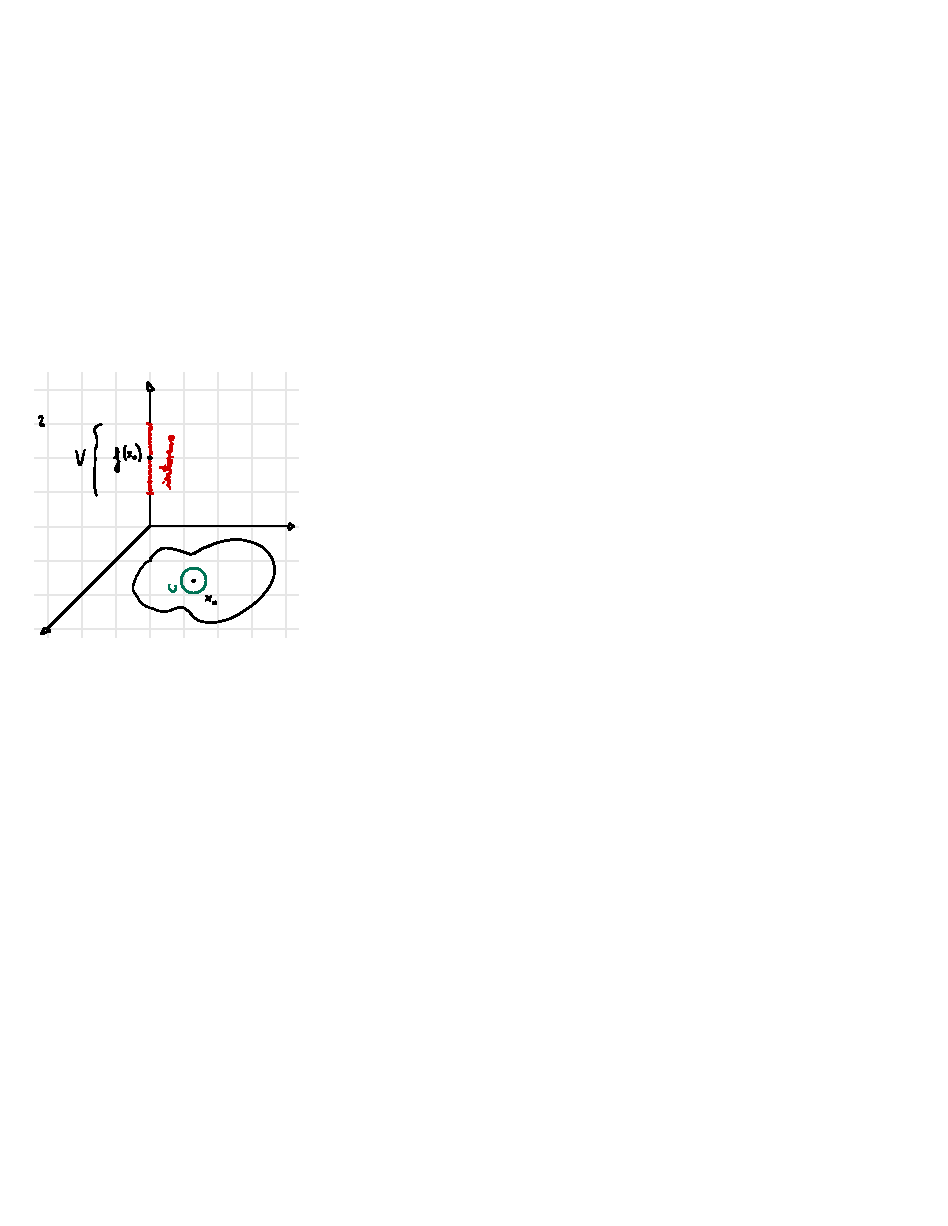
\includegraphics[width=0.5\textwidth]{img/continuita.pdf}
		\caption{$n = 2$.}
	\end{figure}
	
	\noindent
	Qualsiasi punto, che appartiene alla palla, preso in considerazione ritornerà il valore della funzione in quel punto $f\left(x_{0}\right)$.\newline
	
	\noindent
	\textcolor{Red3}{\textbf{\underline{Notazione $\varepsilon$ - $\delta$}}}\newline
	
	\noindent
	Si utilizza una speciale notazione per mostrare una definizione:
	
	\begin{equation*}
		\forall\varepsilon > 0 \hspace{1em} \exists\delta > 0 : \underbrace{\left|f\left(x\right) - f\left(x_{0}\right)\right|}_{\mathbb{R}} < \varepsilon \hspace{1em} \text{se } \overbrace{\Big||x-x_{0}|\Big|}^{\mathbb{R}^{n}} < \delta \hspace{2em} \text{con } x \in D
	\end{equation*}

	\noindent
	Da questa definizione si osserva che:
	
	\begin{itemize}
		\item $\forall\varepsilon > 0$, rappresenta il \textbf{raggio dell'intervallo}.
		
		\item $\exists\delta > 0$, rappresenta il \textbf{raggio della palla}.
		
		\item $\left|f\left(x\right) - f\left(x_{0}\right)\right|$, rappresenta il valore della funzione trovato meno il valore della funzione nel punto $x_{0}$. Il risultato della differenza deve essere minore del raggio dell'intervallo. Quindi, i valori cadono nell'intervallo stabilito.
		
		\item $\text{se } \Big||x-x_{0}|\Big| < \delta$, se $x$ appartiene alla palla di raggio $\delta$.
	\end{itemize}

	\noindent
	Grazie a questa notazione si evince che nei punti isolati del dominio di una generica funzione, la continuità è presente.
	Quindi, \textcolor{Red3}{\textbf{\underline{in ogni punto isolato della}}} \textcolor{Red3}{\textbf{\underline{funzione, essa è continua}}}.
	
	\newpage
	
	\subsubsection{Applicazione della continuità}
	
	\textcolor{Red3}{\textbf{\emph{\underline{Richiesta}}}}\newline
	
	\noindent
	Dimostrare che un'applicazione lineare di $\mathbb{R}^{n}$ è continua in ogni punto $x_{0} \in \mathbb{R}^{n}$.\newline
	
	\noindent
	\textcolor{Green4}{\textbf{\underline{\emph{Risoluzione}}}}\newline
	
	\noindent
	Una funzione lineare $f$ è:
	
	\begin{equation*}
		\begin{array}{lll}
			\mathbb{R}^{n}	& \longrightarrow & \mathbb{R} \\
			x				& \longmapsto	  & a_{1}x_{1} + a_{2}x_{2} + \cdots + a_{n}x_{n} = a \cdot x
		\end{array}
	\end{equation*}

	\noindent
	Con $x$ che rappresenta un vettore. Inoltre, la funzione è definita con $a = \left(a_{1}, a_{2}, ..., a_{n}\right)$ e $x = \left(x_{1}, x_{2}, ..., x_{n}\right)$.\newline
	
	\noindent
	Si studia il valore della funzione in un certo punto:
	
	\begin{equation*}
		\underbrace{\left|ax - ax_{0}\right|}_{\left|f\left(x\right) - f\left(x_{0}\right)\right|} = \left|a \cdot \left(x-x_{0}\right)\right|
	\end{equation*}

	\noindent
	Grazie alla \textcolor{Red3}{\textbf{disuguaglianza triangolare di Cauchy-Schwarz}} (pagina \pageref{disuguaglianza triangolare di cauchy-schwarz}), la funzione è possibile riscriverla come:
	
	\begin{equation*}
		\begin{array}{lll}
			\text{Definizione}	& \longrightarrow & \left|x \cdot y\right| \le \Big||x|\Big| \cdot \Big||y|\Big| \\
			&& \\
			\text{Sostituzione}	& \longrightarrow & \left|a \cdot \left(x-x_{0}\right)\right| \le \Big||a|\Big| \cdot \Big||x-x_{0}|\Big|
		\end{array}
	\end{equation*}

	\noindent
	In cui $\left|x \cdot y\right|$ rappresenta il prodotto scalare assoluto tra due vettori, mentre $\Big||x|\Big| \cdot \Big||y|\Big|$ rappresenta il prodotto in $\mathbb{R}$ di norme tra due vettori.\newline
	
	\noindent
	Quindi $\forall\varepsilon > 0$, il delta è pari a:
	
	\begin{equation*}
		\delta = \dfrac{\varepsilon}{\Big||a|\Big|}
	\end{equation*}

	\noindent
	E riscrivendo la disuguaglianza:
	
	\begin{equation*}
		\Big||a|\Big| \cdot \Big||x-x_{0}|\Big| < \cancel{\Big||a|\Big|} \cdot \dfrac{\varepsilon}{\cancel{\Big||a|\Big|}} = \varepsilon
	\end{equation*}

	\noindent
	Il risultato ottenuto \textbf{non è banale}. Inoltre, questo vale nel caso in cui $a \ne 0$ poiché in caso contrario, ovvero nel caso in cui $a = 0$, la funzione è chiaramente \textbf{continua}.
	
	\newpage
	
	\noindent
	\textcolor{Red3}{\textbf{\underline{\emph{Richiesta 2}}}}\newline
	
	\noindent
	Dimostrare che la funzione $f\left(x,y\right) = e^{x}$ è continua in $\mathbb{R}^{2}$.\newline
	
	\noindent
	\textcolor{Green4}{\textbf{\underline{\emph{Risoluzione}}}}\newline
	
	\noindent
	Si ipotizzi che la funzione $\phi\left(x\right) = e^{x}$ è continua in $\mathbb{R}$. Allora:
	
	\begin{equation*}
		\forall\varepsilon > 0 \hspace{1em} \exists\delta > 0 : \Big|e^{x} - e^{x_{0}}\Big|<\varepsilon \hspace{1em} \text{se } |x-x_{0}| < \delta
	\end{equation*}

	\noindent
	Tuttavia, si osservi che:
	
	\begin{equation*}
		|x-x_{0}| \le \sqrt{\left(x-x_{0}\right)^{2} + \left(y - y_{0}\right)^{2}}
	\end{equation*}

	\noindent
	Ma attenzione! Quella sotto radice è la normale:
	
	\begin{equation*}
		|x-x_{0}| \le \sqrt{\left(x-x_{0}\right)^{2} + \left(y - y_{0}\right)^{2}} = \Big|\left|\left(x,y\right) - \left(x_{0}, y_{0}\right)\right|\Big|
	\end{equation*}

	\noindent
	Allora, si conclude l'esercizio con:
	
	\begin{equation*}
		\forall\varepsilon \hspace{1em} \exists\delta > 0 : \Big|\left|\left(x,y\right) - \left(x_{0}, y_{0}\right)\right|\Big| < \delta
	\end{equation*}

	\noindent
	In altre parole, si prende una coppia $x,y$ più piccola di $\delta$. Nel caso in cui questa condizione viene rispettata, allora:
	
	\begin{equation*}
		\left|e^{x} - e^{x_{0}}\right| = \left|f\left(x,y\right) - f\left(x_{0}, y_{0}\right)\right| < \varepsilon
	\end{equation*}

	\noindent
	La differenza è minore di $\varepsilon$, nonché uguale a $e^{x} - e^{x_{0}}$.
	
	\newpage
	
	\subsubsection{Proprietà delle funzioni continue ed \textcolor{Red3}{esame}}
	
	Se $f,g$ sono funzioni continue su $A \subseteq \mathbb{R}^{n}$, allora:
	
	\begin{itemize}[label=-]
		\item $f + g$, la \textbf{somma} delle due funzioni è continua su $A$.
		\item $f - g$, la \textbf{differenza} delle due funzioni è continua su $A$.
		\item $f \cdot g$, la \textbf{moltiplicazione} delle due funzioni è continua su $A$.
		\item $\dfrac{f}{g}$, la \textbf{divisione} è una funzione continua su $A \setminus \left\{x \in A : g\left(x\right) = 0\right\}$. Ovvero, nell'insieme non ci devono essere zeri.
	\end{itemize}
	
	\noindent
	Se $f$ è una funzione continua su $A \subseteq \mathbb{R}^{n}$ e la funzione $g$ è continua sull'intervallo $I \subseteq \mathbb{R}$, allora l'operazione \dquotes{\textbf{composto}} è continua sul dominio:
	
	\begin{equation*}
		D = \left\{x \in A: f\left(x\right) \in I\right\}
	\end{equation*}
	
	\noindent
	Il dominio indica che i valori \emph{devono} stare all'interno di $A$ per iniziare il processo. Tuttavia, è ammessa anche l'immagine, dei valori, per far processare la funzione $g$.\newline
	L'operazione \textcolor{Red3}{\dquotes{\textbf{\underline{composto}}}} è formalmente scritta come $h = f \circ g$ e indica che la funzione $f$ riceve dei vettori ($\mathbb{R}^{n}$) e restituisce valori reali i quali saranno processati dalla funzione $g$.\newline
	
	\noindent
	\textcolor{Red3}{\textbf{\underline{\emph{All'esame...}}}}\newline
	
	\noindent
	Ipotizzando un esercizio del tipo, si dimostri la continuità della funzione:
	
	\begin{equation*}
		f\left(x,y\right) = x \cdot \dfrac{e^{x^{2} + y^{2}} - 1}{x^{2} + y^{2} + 1}
	\end{equation*}

	\noindent
	Si ricava il dominio della funzione, in questo caso $D_{f} = \mathbb{R}^{2}$ e si conclude l'esercizio dicendo che la funzione $f$ è continua in $\mathbb{R}^{2}$ poiché si ottiene combinando funzioni continue su $\mathbb{R}^{2}$.
	
	\newpage
	
	\subsection{Limiti}
	
	Sia $f: D \subseteq \mathbb{R}^{n} \longrightarrow \mathbb{R}$ e sia $x_{0}$ un punto di accumulazione per $D$, si definisce il limite:
	
	\begin{equation*}
		\lim_{x \rightarrow x_{0}} f\left(x\right) = L \hspace{1em} \text{se } \forall\varepsilon > 0 \hspace{1em} \exists\delta > 0 : \left|f\left(x\right) - L\right| < \varepsilon \hspace{1em} \forall x \in D, 0 < \Big|\left|x - x_{0}\right|\Big| < \delta
	\end{equation*}
	
	\noindent
	In cui:
	
	\begin{itemize}
		\item $\Big|f\left(x\right) - L\Big| < \varepsilon$, rappresenta la distanza tra i valori della funzione e il valore limite $L$ e si impone che sia minore di $\varepsilon$. Questo vale solo nel caso in cui $x$ è nel dominio e sia vicino $\delta$ ma \textbf{non negativo o zero!} \textcolor{Red3}{\textbf{Punti isolati non hanno limiti}}.
		
		\item $0 < \Big||x-x_{0}|\Big|$, vuol dire che $x \ne x_{0}$.
	\end{itemize}
	
	\noindent
	\textcolor{Red3}{\textbf{\underline{Nota}}}\newline
	
	\noindent
	La funzione $f$ è continua nel punto $x_{0}$ se:
	
	\begin{enumerate}[label=\alph*)]
		\item $x_{0} \in D'$, dove $x_{0}$ è un punto di accumulazione e $D'$ indica gli insiemi dei punti di accumulazione. La continuità esiste se:
		\begin{equation*}
			\lim_{x \rightarrow x_{0}} f\left(x\right) = f\left(x_{0}\right)
		\end{equation*}
	
		\item $x_{0}$ è un punto isolato.
	\end{enumerate}

	\noindent
	\textcolor{Red3}{\textbf{Valgono tutti i seguenti teoremi \underline{sui limiti} per funzioni di \underline{una sola variabile}:}}
	
	\noindent
	\begin{itemize}[label=-]
		\item Unicità
		\item Permanenza del segno
		\item Confronto
		\item Somma, prodotto, ecc.
	\end{itemize}

	\newpage
	
	\subsubsection[Esempio introduttivo]{\textcolor{Green4}{Esempio introduttivo}}
	
	Calcolare, se esiste, il limite:
	
	\begin{equation*}
		\lim_{\left(x,y\right) \rightarrow \left(0,0\right)} \dfrac{x^{3} + y^{2}}{x^{2} + y^{2}}
	\end{equation*}

	\noindent
	La \textbf{risoluzione} dei limiti prevede di \textbf{provare a dimostrare che essi non esistono}. Quindi, se si riesce a trovare due limiti, con cammini diversi, che portano a risultati diversi, allora il limite non esiste.\newline
	
	\noindent
	\textcolor{Green4}{\textbf{Per esempio}}, nel seguente caso i percorsi scelti sono lungo gli assi:
	
	\begin{figure}[!htp]
		\centering
		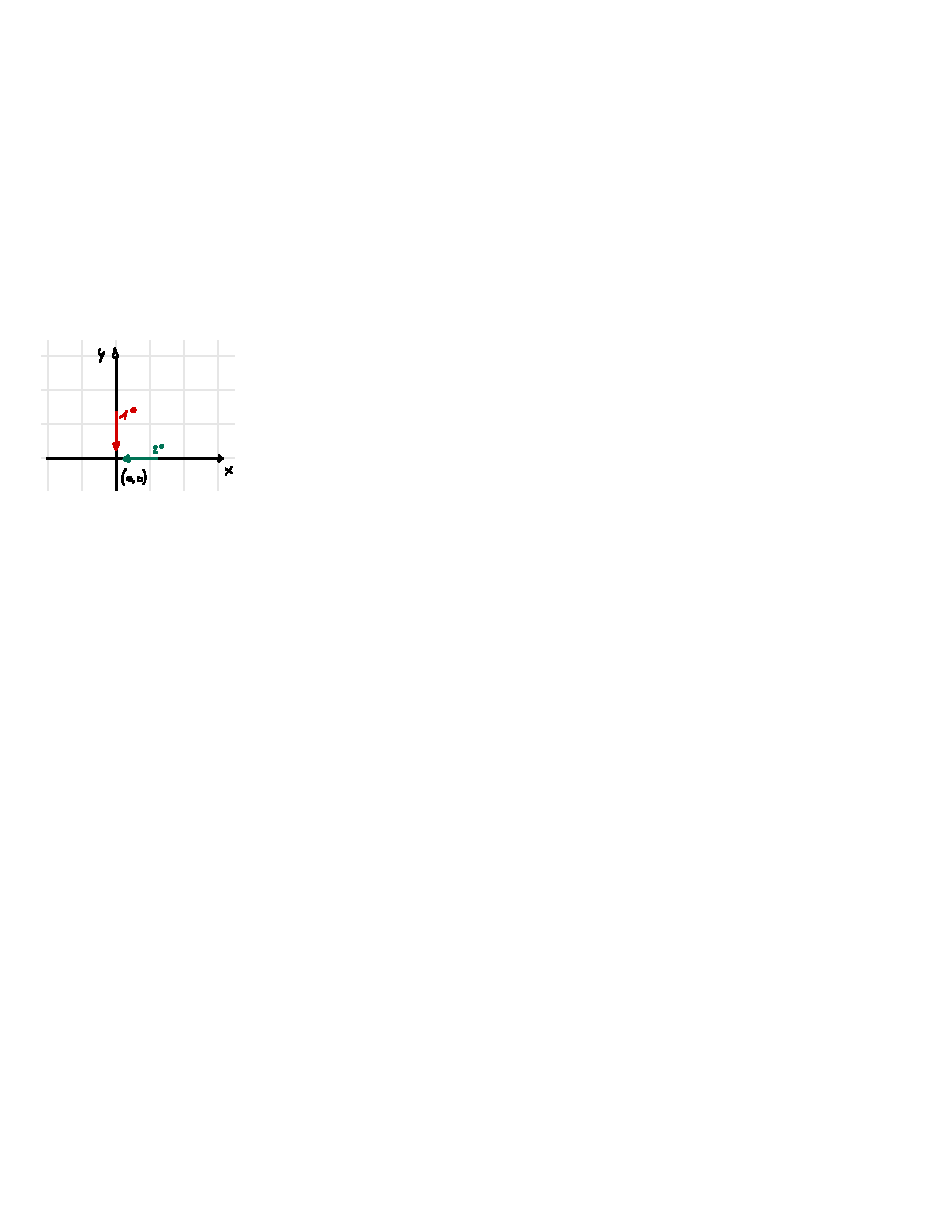
\includegraphics[width=0.5\textwidth]{img/limiti.pdf}
		\caption{In rosso il 1° percorso e in verde il 2° percorso.}
	\end{figure}
	
	\noindent
	\textcolor{Red3}{\textbf{\underline{1° percorso:}}}
	
	\begin{equation*}
		\lim_{y \rightarrow 0} f\left(0,y\right) = \lim_{y \rightarrow 0} \dfrac{y^{2}}{y^{2}} = 1
	\end{equation*}

	\noindent
	In cui la funzione $f\left(0,y\right)$ rappresenta la restrizione di $f$ nei punti dell'asse $y$.\newline
	
	\noindent
	\textcolor{Green4}{\textbf{\underline{2° percorso:}}}
	
	\begin{equation*}
		\lim_{x \rightarrow 0} f\left(x,0\right) = \lim_{x \rightarrow 0} \dfrac{x^{3}}{x^{2}} = 0
	\end{equation*}
	
	\noindent
	L'esercizio si conclude dicendo che $\lim_{y \rightarrow 0}f\left(0y\right) \ne \lim_{x \rightarrow 0}f\left(x,0\right)$, ovvero che il risultato è diverso. Quindi, per definizione \textbf{\underline{non esiste}}:
	
	\begin{equation*}
		\lim_{\left(x,y\right) \rightarrow \left(0,0\right)} f\left(x,y\right)
	\end{equation*}

	\newpage

	\subsubsection[Esempio 1]{\textcolor{Green4}{Esempio 1}}
	
	Data la funzione:
	
	\begin{equation*}
		\begin{cases}
			x \cdot e^{\frac{x}{y}}	& y \ne 0 \\
			0						& y = 0
		\end{cases}
	\end{equation*}

	\noindent
	Calcolare, se esiste, il limite:
	
	\begin{equation*}
		\lim_{\left(x,y\right) \rightarrow \left(0,0\right)} f\left(x,y\right)
	\end{equation*}

	\noindent
	Si noti bene che la funzione è nulla sull'asse delle $y$.\newline
	
	\noindent
	Come nell'esercizio del paragrafo precedente, si provano i vari percorsi. Quindi, \textbf{lungo $\boldsymbol{y}$} è pari a zero:
	
	\begin{equation*}
		\lim_{x \rightarrow 0} f\left(x,0\right) = 0
	\end{equation*}

	\noindent
	Analogamente, lungo $x$ deve essere $0$ per far esistere il limite della funzione. Dunque, \textbf{lungo $\boldsymbol{x}$} è:
	
	\begin{equation*}
		\lim_{y \rightarrow 0} f\left(0,y\right) = 0 \cdot e^{\frac{0}{y}} = 0
	\end{equation*}

	\noindent
	Nonostante sia evidente che il limite esiste, è possibile effettuare una verifica ulteriore tramite una retta passante l'origine $\left(0,0\right)$.
	
	\begin{figure}[!htp]
		\centering
		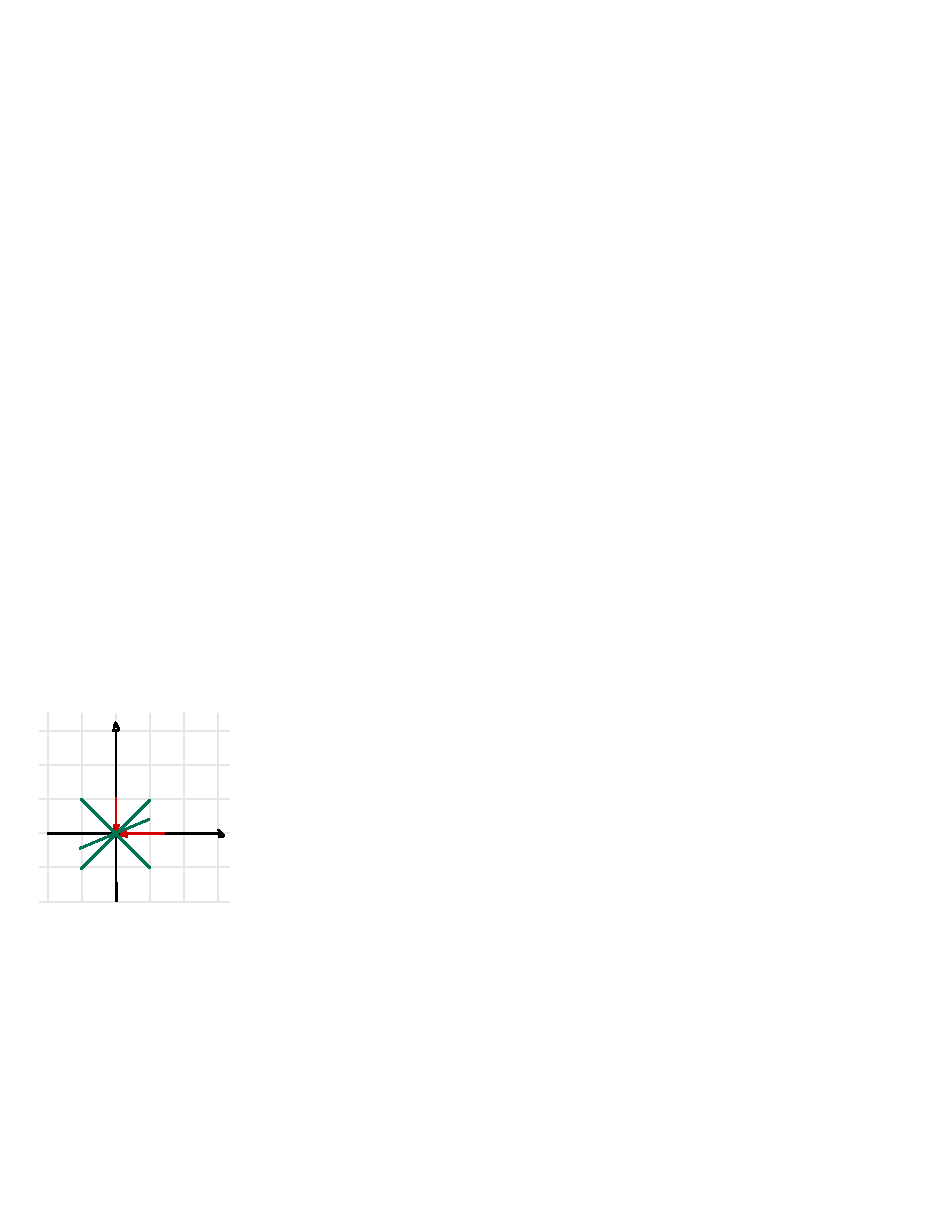
\includegraphics[width=0.5\textwidth]{img/limiti_ex1.pdf}
		\caption{Retta passante per l'origine.}
	\end{figure}

	\noindent
	La retta è definita con la seguente funzione:
	
	\begin{equation*}
		f\left(x, mx\right) = x \cdot e^{\frac{\cancel{x}}{m\cancel{x}}} = x \cdot e^{\frac{1}{m}}
	\end{equation*}

	\noindent
	In cui $f\left(x, mx\right)$ indica la restrizione della funzione $f$ lungo la retta per l'origine. Infatti:
	
	\begin{equation*}
		\lim_{x \rightarrow 0} x \cdot e^{\frac{1}{m}} = 0
	\end{equation*}

	\noindent
	Nonostante la prova ulteriore, il risultato continua ad essere zero. Tuttavia, adesso si prova con una parabola.
	
	\begin{figure}[!htp]
		\centering
		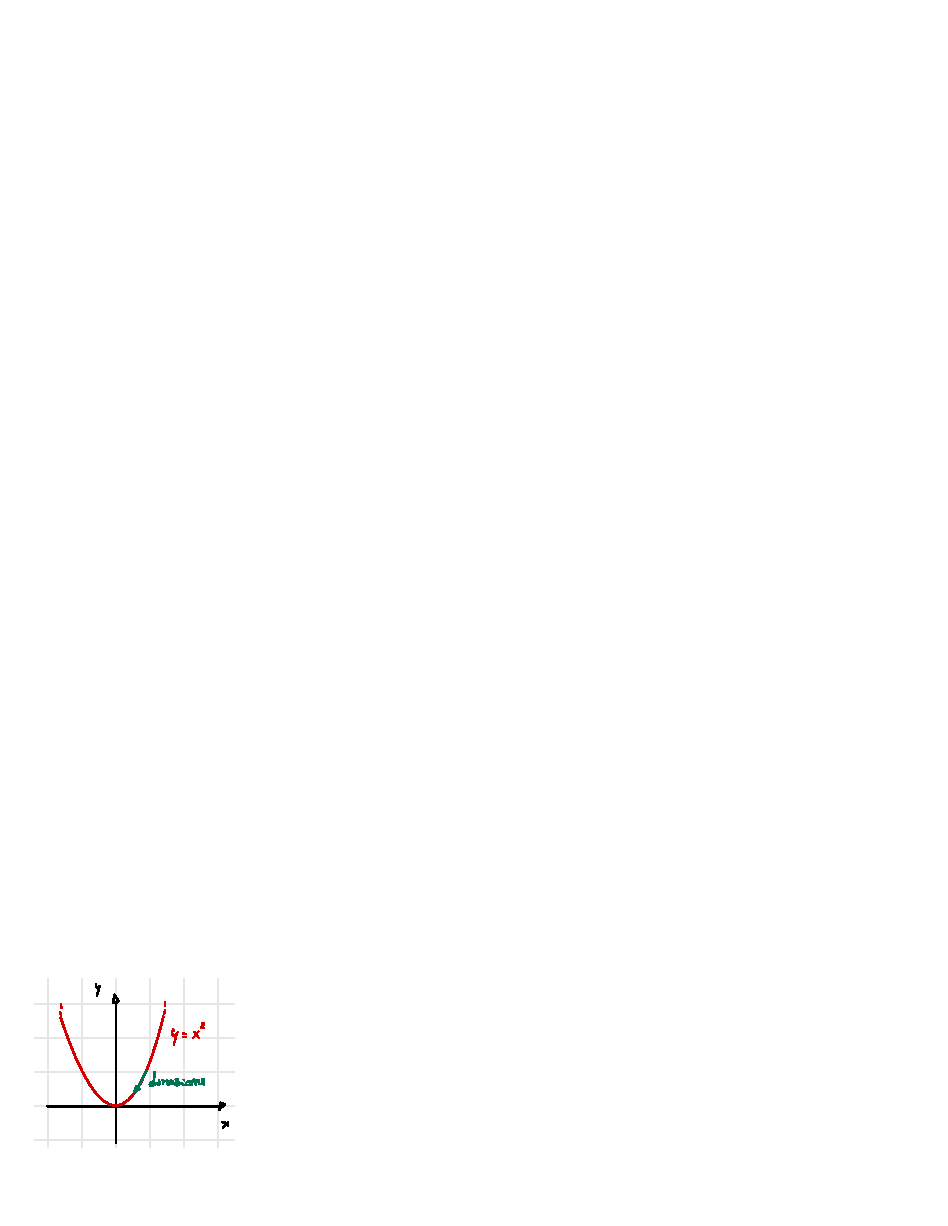
\includegraphics[width=0.5\textwidth]{img/limiti_ex2.pdf}
	\end{figure}

	\noindent
	La funzione restrizione è la seguente:
	
	\begin{equation*}
		f\left(x,x^{2}\right) = x e^{\frac{x}{x^{2}}} = xe^{\frac{1}{x}}
	\end{equation*}

	\noindent
	Il limite diventa dunque:
	
	\begin{equation*}
		\lim_{x \rightarrow 0^{+}} x \cdot e^{\frac{1}{x}} = +\infty
	\end{equation*}

	\noindent
	Il risultato \textbf{non} è zero e dunque si conclude che il \textbf{limite non esiste}.
	
	\newpage
	
	\subsubsection[Esempio 2]{\textcolor{Green4}{Esempio 2}}
	
	Si provi che non esiste il limite:
	
	\begin{equation*}
		\lim_{\left(x,y\right) \rightarrow \left(0,0\right)} \dfrac{xy}{x^{2} + y^{2}}
	\end{equation*}

	\noindent
	Si effettuano le prove lungo gli assi $x$ e $y$:
	
	\begin{equation*}
		\lim_{y \rightarrow 0}f\left(0,y\right) = \lim_{x \rightarrow 0} f\left(x,0\right) = 0
	\end{equation*}

	\noindent
	Il risultato è sempre zero, dunque si prova lungo la bisettrice con il coefficiente $m$ uguale a $1$:
	
	\begin{equation*}
		\lim_{x \rightarrow 0} f\left(x,x\right) = \dfrac{x \cdot x}{x^{2} + x^{1}} = \dfrac{\cancel{x^{2}}}{2 \cancel{x^{2}}} = \dfrac{1}{2}
	\end{equation*}

	\noindent
	L'esercizio si conclude, poiché il risultato è diverso da zero e dunque il limite non esiste.
	
	\newpage
	
	\subsubsection[Esempio, verifica della continuità]{\textcolor{Green4}{Esempio, verifica della continuità}}
	
	Data la funzione:
	
	\begin{equation*}
		f\left(x,y\right) =
		\begin{cases}
			\dfrac{x^{4} + y^{4}}{x^{2} + y^{2}}	& \text{se } \left(x,y\right) \ne \left(0,0\right) \\
			0										& \text{se }\left(x,y\right) = \left(0,0\right)
		\end{cases}
	\end{equation*}

	\noindent
	Si determini se la funzione è continua in $\left(0,0\right)$.\newline
	
	\noindent
	È necessario verificare che:
	
	\begin{equation*}
		\lim_{\left(x,y\right) \rightarrow \left(0,0\right)} f\left(x,y\right) = f\left(0,0\right) = 0
	\end{equation*}

	\noindent
	Si utilizza la \textcolor{Red3}{\textbf{\underline{tecnica del confronto}}} costruendo una maggiorazione:
	
	\begin{equation*}
		\text{se } \left(x,y\right) \ne \left(0,0\right) \Longrightarrow 0 \le \dfrac{x^{4} + y^{4}}{x^{2} + y^{2}} \le \underbrace{\dfrac{\left(x^{2} + y^{2}\right)^{2}}{x^{2} + y^{2}}}_{\text{maggiorazione}} = x^{2} + y^{2}
	\end{equation*}

	\noindent
	Adesso si verifica il limite:
	
	\begin{equation*}
		\lim_{\left(x,y\right) \rightarrow \left(0,0\right)} x^{2} + y^{2} = 0
	\end{equation*}

	\noindent
	Il limite è uguale a zero e dunque la funzione è continua.
	
	\newpage
	
	\subsubsection[Esempio 3]{\textcolor{Green4}{Esempio 3}}
	
	Calcolare se esiste il limite:
	
	\begin{equation*}
		\lim_{\left(x,y\right) \rightarrow \left(0,0\right)} f\left(x,y\right) = \dfrac{x^{2}}{\sqrt{x^{2} + y^{2}}}
	\end{equation*}

	\noindent
	Si utilizza il \textbf{teorema del confronto} come nel paragrafo precedente e si ottiene:
	
	\begin{equation*}
		0 \le \dfrac{x^{2}}{\sqrt{x^{2} + y^{2}}} \le \dfrac{x^{2} + y^{2}}{\sqrt{x^{2} + y^{2}}} = \sqrt{x^{2} + y^{2}}
	\end{equation*}

	\noindent
	Si applica il limite alla funzione dopo la maggiorazione:
	
	\begin{equation*}
		\lim_{\left(x,y\right) \rightarrow \left(0,0\right)} \sqrt{x^{2} + y^{2}}
	\end{equation*}

	\newpage
	
	\subsection{Sintesi delle maggiorazioni}
	
	Qui di seguito viene lasciato un elenco di maggiorazioni:
	
	\begin{itemize}
		\item $|x| \le \sqrt{x^{2} + y^{2}}$
		\item $|xy| \le \dfrac{1}{2}\left(x^{2} + y^{2}\right)$
		\item $|\sin \left(x\right)| \le |x|$
	\end{itemize}

	\newpage
	
	\section{Lezione 10}
	
	\subsection{Esempi}
	
	\subsubsection[Esempio 1]{\textcolor{Green4}{Esempio 1}}
	
	Verificare che il limite è uguale a $0$:
	
	\begin{equation*}
		\lim_{\left(x,y\right) \rightarrow \left(0,0\right)} \dfrac{\sin\left(x,y\right)}{\sqrt{|xy|}} = 0
	\end{equation*}

	\noindent
	Il dominio della funzione è:
	
	\begin{equation*}
		D_{f} = \left\{\left(x,y\right) \in \mathbb{R}^{2} : x \cdot y \ne 0\right\}
	\end{equation*}

	\noindent
	Il grafico del dominio corrisponde a:
	
	\begin{figure}[!htp]
		\centering
		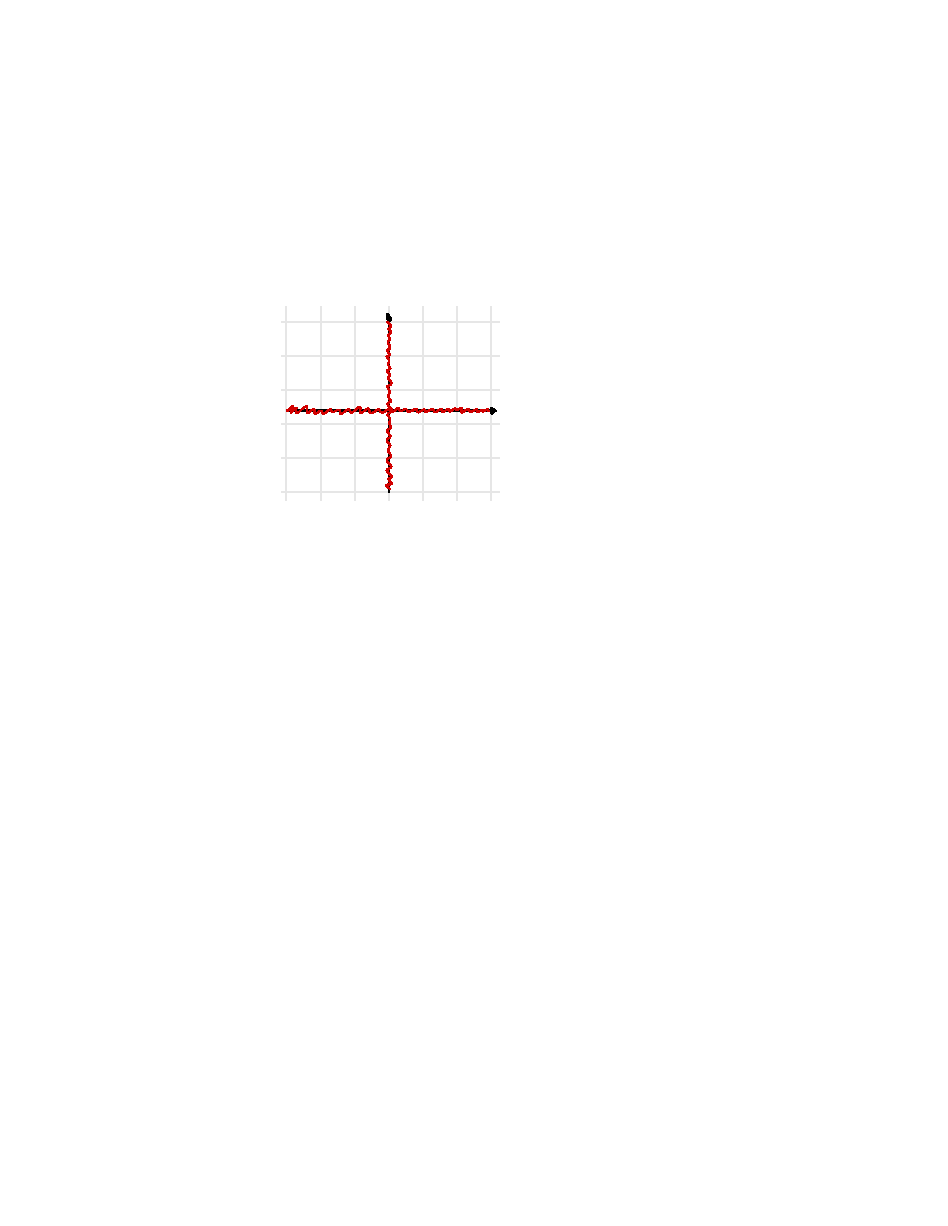
\includegraphics[width=0.5\textwidth]{img/limiti_ex3.pdf}
	\end{figure}

	\noindent
	La linea rossa indica che il dominio è definito ovunque nello spazio eccetto sugli assi.\newline
	
	\noindent
	Per verificare l'esistenza del limite si utilizza la \textbf{tecnica del confronto} facendo maggiorazioni:
	
	\begin{equation*}
		0 \le \left|\dfrac{\sin\left(x,y\right)}{\sqrt{|xy|}}\right| \le \dfrac{|xy|}{\sqrt{|xy|}} \xrightarrow{\text{grazie alla razionalizzazione}} \: = \sqrt{|xy|}
	\end{equation*}

	\noindent
	Applicando il valore trovato al limite:
	
	\begin{equation*}
		\lim_{\left(x,y\right) \rightarrow \left(0,0\right)} \sqrt{|xy|} = 0
	\end{equation*}

	\noindent
	Si conclude affermando che il limite è uguale a zero.
	
	\newpage
	
	\subsubsection[Esempio 2]{\textcolor{Green4}{Esempio 2}}
	
	Verificare l'esistenza del limite:
	
	\begin{equation*}
		\lim_{\left(x,y\right) \rightarrow \left(1,0\right)} \dfrac{\left(x-1\right)^{2} + y^{2}}{1-x^{2}-y^{2}}
	\end{equation*}

	\noindent
	Per farlo, si verifica sull'asse $x$, dato che che $y = 0$:
	
	\begin{equation*}
		f\left(x,0\right) = \dfrac{\left(x-1\right)^{2} + 0^{2}}{1-x^{2}-0^{2}} = \dfrac{\left(x-1\right)^{2}}{1-x^{2}} = \dfrac{\left(x-1\right)^{\cancel{2}}}{\left(x+1\right)\cancel{\left(x-1\right)}}
	\end{equation*}

	\noindent
	Si applica il valore al limite:
	
	\begin{equation*}
		\lim_{x \rightarrow 1} \dfrac{\left(x-1\right)}{\left(x+1\right)} = 0
	\end{equation*}

	\noindent
	Provando a sostituire $x = 1$ nella funzione:
	
	\begin{equation*}
		f\left(1,y\right) = \dfrac{\cancel{\left(x-1\right)^{2}} + y^{2}}{\cancel{1 - x^{2}} - y^{2}} = -\dfrac{y^{2}}{y^{2}} = -1
	\end{equation*}

	\noindent
	I risultato è diverso da zero, dunque \textbf{il limite non esiste}.
	
	\begin{figure}[!htp]
		\centering
		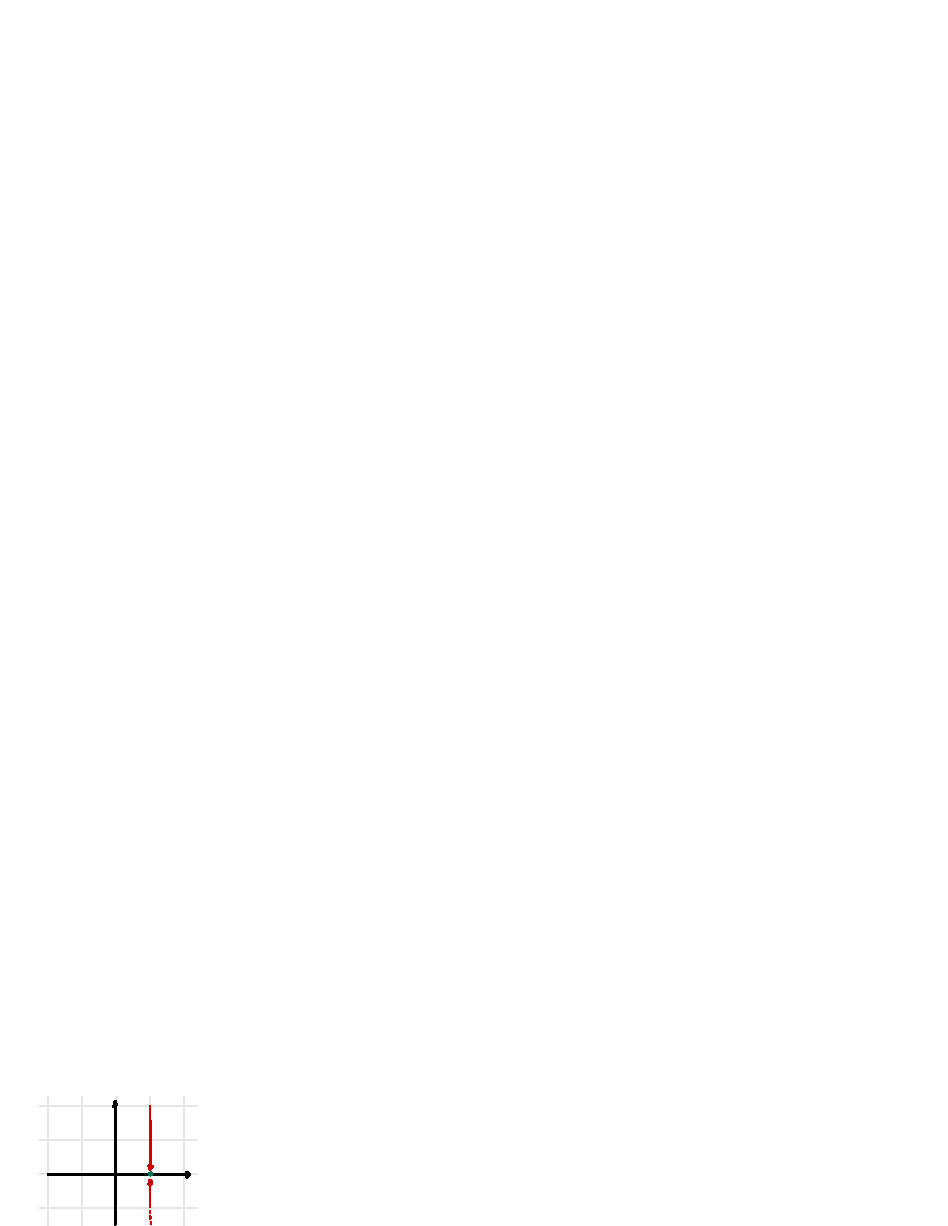
\includegraphics[width=0.5\textwidth]{img/limiti_ex4.pdf}
		\caption{Grafico della funzione con $x = 1$.}
	\end{figure}

	\newpage
	
	\subsection{Calcolo di limiti con coordinate polari}
	
	Le coordinate polari sono una notazione che prevede che nell'asso cartesiano $x,y$, ci sia un punto polare $P$ identificato dalle coordinate polari $x_{P},y_{P}$, da un angolo $\theta$ e da un raggio $r$.
	
	\begin{figure}[!htp]
		\centering
		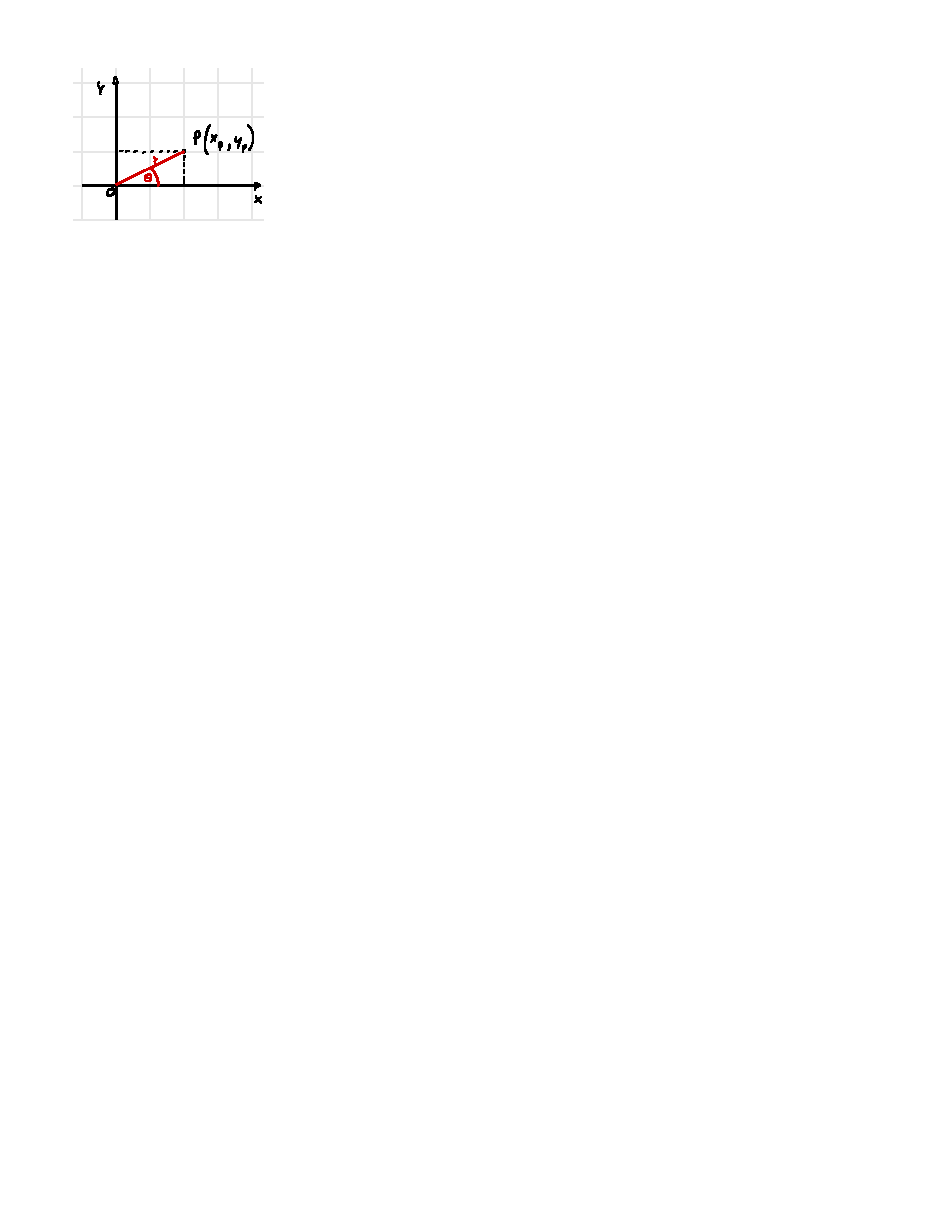
\includegraphics[width=0.4\textwidth]{img/limiti_con_coordinate_polari.pdf}
		\caption{Rappresentazione delle coordinate polari nell'origine.}
	\end{figure}

	\noindent
	Le formule per calcolare i vari punti sono:
	
	\begin{itemize}
		\item La distanza $r$, calcolata come la distanza tra l'origine e il punto $P$. Formalmente $r = \overline{OP}$
		
		\item La componente $x$, calcolata come $x = r \cdot \cos\left(\theta\right)$
		
		\item La componente $y$, calcolata come $y = r \cdot \sin\left(\theta\right)$
	\end{itemize}

	\noindent
	Nel caso in cui l'origine del punto polare \textbf{non} è l'origine degli assi cartesiani, allora le formule sono diverse.
	
	\begin{figure}[!htp]
		\centering
		\includegraphics[width=0.4\textwidth]{img/limiti_con_coordinate_polari2.pdf}
		\caption{Rappresentazione delle coordinate polari in un punto diverso dall'origine.}
	\end{figure}
	
	\noindent
	Le formule per calcolare i vari punti sono:
	
	\begin{itemize}
		\item La distanza $r$, la formula rimane invariata, sempre la distanza tra i due punti
		
		\item La componente $x$, calcolata come $x = x_{P} + r \cos\left(\theta\right)$
		
		\item La componente $y$, calcolata come $y = y_{P} + r \sin\left(\theta\right)$
	\end{itemize}

	\newpage
	
	\noindent
	Il calcolo dei limiti con coordinate polari prevede di definire la funzione $F$ come:
	
	\begin{equation*}
		F\left(r,\theta\right) = f\left(x_{P} + r \cdot \cos\left(\theta\right), y_{P} + r \cdot \sin\left(\theta\right)\right)
	\end{equation*}

	\noindent
	Allora, se il suo limite:
	
	\begin{equation*}
		\lim_{r \rightarrow 0^{+}} F\left(r,\theta\right) = L \in \mathbb{R}
	\end{equation*}

	\noindent
	È \textcolor{Red3}{\textbf{\underline{uniformemente rispetto a $\theta$}}}, allora si ha:
	
	\begin{equation*}
		\lim_{\left(x,y\right) \rightarrow \left(x_{P}, y_{P}\right)} f\left(x,y\right) = L
	\end{equation*}

	\newpage
	
	\subsubsection[Esempio di non uniformità]{\textcolor{Green4}{Esempio di non uniformità}}
	
	Verificare che il limite esista:
	
	\begin{equation*}
		\lim_{\left(x,y\right) \rightarrow \left(0,0\right)} \dfrac{xy^{2}}{x^{2} + y^{4}}
	\end{equation*}

	\noindent
	Con il caso $x=0$ e l'analogo caso con $y=0$, il limite tende a zero:
	
	\begin{equation*}
		\lim_{y \rightarrow 0} f\left(0,y\right) = \lim_{x \rightarrow 0} f\left(x,0\right) = 0
	\end{equation*}

	\noindent
	Applicando le coordinate polari, si ottiene la funzione $F$, definita:
	
	\begin{equation*}
		F\left(r,\theta\right) = \dfrac{r \cdot \cos\left(\theta\right) \cdot \left(r \cdot \sin\left(\theta\right)\right)^{2}}{\left(r \cdot \cos\left(\theta\right)\right)^{2} + \left(r \cdot \sin\left(\theta\right)\right)^{2}} = \dfrac{r^{3} \cdot \cos\left(\theta\right) \cdot \sin^{2}\left(\theta\right)}{r^{2} \cdot \cos^{2}\left(\theta\right) + r^{4} \cdot \sin^{4}\left(\theta\right)} = \dfrac{r \cdot \cos\left(\theta\right) \cdot \sin^{2}\left(\theta\right)}{\cos^{2}\left(\theta\right) + r^{2} \cdot \sin^{4}\left(\theta\right)}
	\end{equation*}

	\noindent
	Se facessimo tendere la funzione $F$ a $r \rightarrow 0^{+}$, si otterrebbe zero come risultato. Tuttavia, in questo caso convergerebbe non uniformemente rispetto a $\theta$, quindi il \textbf{limite non esisterebbe}. In altre parole, in questo caso si avrebbe:
	
	\begin{equation*}
		\forall\varepsilon, \forall\theta \: \exists\delta \text{ tale che...}
	\end{equation*}

	\noindent
	Al contrario, per essere \textbf{uniformemente rispetto a $\theta$}, dovrebbe essere:
	
	\begin{equation*}
		\forall\varepsilon \: \exists\delta \text{ tale che qualunque sia } \theta ...
	\end{equation*}

	\subsubsection[Quando è uniforme rispetto a $\boldsymbol{\theta}$]{\textcolor{Red3}{Quando è uniforme rispetto a $\boldsymbol{\theta}$}}
	
	Se per $\left(x,y\right)$ che tende a $\left(x_{P},y_{P}\right)$ si ha:
	
	\begin{equation*}
		\left|F\left(r,\theta\right) = L\right| \le g\left(r\right)
	\end{equation*}

	\noindent
	Dove la funzione $g\left(r\right)$ ha solo $r$ e dunque $\theta$ non può apparire e il suo limite è zero:
	
	\begin{equation*}
		\lim_{r \rightarrow 0^{+}} g\left(r\right) = 0
	\end{equation*}

	\noindent
	In altre parole è la funzione infinitesima.\newline
	
	\noindent
	Se queste condizioni sono rispettate, allora il limite:
	
	\begin{equation*}
		\lim_{\left(x,y\right) \rightarrow \left(x_{P},y_{P}\right)} f\left(x,y\right) = L
	\end{equation*}

	\newpage
	
	\subsubsection[Esempio 1]{\textcolor{Green4}{Esempio 1}}
	
	Data la funzione:
	
	\begin{equation*}
		f\left(x,y\right) = \dfrac{xy}{\sqrt{x^{2} + y^{2}}}
	\end{equation*}

	\noindent
	Il limite che tede a $\left(0,0\right)$ è:
	
	\begin{equation*}
		\lim_{\left(x,y\right) \rightarrow \left(0,0\right)} \dfrac{xy}{\sqrt{x^{2} + y^{2}}} = 0
	\end{equation*}

	\noindent
	Ed è certo che esiste.\newline
	Si applicano le coordinate polari:
	
	\begin{equation*}
		\begin{array}{lll}
			F\left(r,\theta\right) & = & \left|\dfrac{r \cdot \cos\left(\theta\right) \cdot r \cdot \sin\left(\theta\right)}{\sqrt{r^{2} \cdot \cos^{2}\left(\theta\right) + r^{2} \cdot \sin^{2}\left(\theta\right)}}\right| \\
			&& \\
			& = & \left|\dfrac{r^{\cancel{2}} \cdot \sin\left(\theta\right) \cdot \cos\left(\theta\right)}{\cancel{r}}\right| \\
			&& \\
			& = & \left|r \cdot \sin\left(\theta\right) \cdot \cos\left(\theta\right)\right| \\
			&& \\
			& = & \left|r \cdot \dfrac{1}{2} \cdot \sin\left(\theta\right)\right| \le \dfrac{1}{2}r
		\end{array}
	\end{equation*}

	\noindent
	Dove l'ultima disuguaglianza dà la certezza che per qualsiasi valore di $\theta$, la funzione sarà uguale o minore alla metà del raggio.\newline
	
	\noindent
	Inoltre, l'espressione $\frac{1}{2}r$ rappresenta la funzione $g\left(r\right)$, quindi il limite esiste perché è uniformemente rispetto a $\theta$.
	
	\subsubsection[Esempio 2]{\textcolor{Green4}{Esempio 2}}
	
	Data il limite della funzione:
	
	\begin{equation*}
		\lim_{\left(x,y\right) \rightarrow \left(0,1\right)} \dfrac{x^{2}}{\sqrt{x^{{2} + \left(y-1\right)^{2}}}}
	\end{equation*}

	\noindent
	Le coordinate polari sono:
	
	\begin{equation*}
		\begin{cases}
			x = r \cdot \cos\left(\theta\right) \\
			y = 1 + r \cdot \sin\left(\theta\right)
		\end{cases}
	\end{equation*}

	\noindent
	La funzione $F$ che si ricava è òa seguente:
	
	\begin{equation*}
		\left|F\left(r,\theta\right) - 0\right| = \left|\dfrac{r^{2} \cdot \cos^{2}\left(\theta\right)}{\sqrt{r^{2} \cdot \cos^{2}\left(\theta\right) + \left(1 + r \cdot \sin\left(\theta\right) - 1\right)^{2}}}\right| = \left|\dfrac{r^{2} \cdot \cos^{2}\left(\theta\right)}{r}\right| = r \cdot \cos^{2}\left(\theta\right) \le r
	\end{equation*}

	\noindent
	In cui $r$ rappresenta la funzione $g\left(r\right)$. Il limite dunque è:
	
	\begin{equation*}
		\lim_{r \rightarrow 0^{+}} g\left(r\right) = 0
	\end{equation*}

	\newpage
	
	\subsubsection[Esempio 3 - Difficile]{\textcolor{Green4}{Esempio 3 - Difficile}}
	
	Dato il limite della funzione:
	
	\begin{equation*}
		\lim_{\left(x,y\right) \rightarrow \left(1,2\right)} \dfrac{\log\left(3 - 2x -y + xy\right)}{\sqrt{x^{2} + y^{2} - 2x -4y + 5}}
	\end{equation*}

	\noindent
	Sicuramente con le rette a zero, il limite è zero. Quindi, si calcolano le coordinate polari:
	
	\begin{equation*}
		\begin{cases}
			x = 1 + r \cdot \cos\left(\theta\right) \\
			y = 2 + r \cdot \sin\left(\theta\right)
		\end{cases}
	\end{equation*}

	\noindent
	La relativa funzione è:
	
	\begin{gather*}
		\left|F\left(r,\theta\right) - 0\right| = \\
		\\
		\left|\dfrac{\log\left(3 - 2 - 2 \cdot r \cdot \cos\left(\theta\right) - 2 - r \cdot \sin\left(\theta\right) + 2 + r \cdot \sin\left(\theta\right) + 2 \cdot r \cdot \cos\left(\theta\right) + r^{2} \cdot \sin\left(\theta\right) \cdot \cos\left(\theta\right)\right)}{r}\right| = \\
		\\
		= \left|\dfrac{\log\left(1 + r^{2} \cdot \sin\left(\theta\right) \cdot \cos\left(\theta\right)\right)}{r}\right|
	\end{gather*}

	\noindent
	Dato il logaritmo fondamentale:
	
	\begin{equation*}
		\begin{array}{lll}
			& \longrightarrow & \lim_{t \rightarrow 0} \dfrac{\log\left(1+t\right)}{t} = 1 \\
			&& \\
			\text{Con la tecnica di maggiorazione} & \longrightarrow & \left|\dfrac{\log\left(1+t\right)}{t}\right| \le 2 \\
			&& \\
			\text{Manipolazione utile}			   & \longrightarrow & \left|\log\left(1+t\right)\right| \le 2\left|t\right| \\
		\end{array}
	\end{equation*}

	\noindent
	Si sostituisce (?):
	
	\begin{equation*}
		\left|\dfrac{\log\left(1 + r^{2} \sin\left(\theta\right) \cos\left(\theta\right)\right)}{r}\right| \le \dfrac{2 \cdot \left|r^{2} \sin\left(\theta\right) \cos\left(\theta\right)\right|}{r} \le 2 r \cdot \dfrac{1}{2} = r
	\end{equation*}

	\noindent
	Il risultato è uguale a zero.
	
	\newpage
	
	\subsection{Continuità - Proprietà e teoremi importanti}
	
	\textbf{\emph{Le seguenti definizioni valgono solamente per funzioni continue.}}\newline
	
	\noindent
	Sia $f$ una funzione continua su $\mathbb{R}^{n}$. Allora:
	
	\begin{equation*}
		A_{1} = \left\{x \in \mathbb{R}^{n} : f\left(x\right) > 0\right\}
	\end{equation*}
	
	È un \textcolor{Red3}{\textbf{\underline{insieme aperto}}}. Tuttavia, lo è anche:
	
	\begin{equation*}
		A_{2} = \left\{x \in \mathbb{R}^{n} : f\left(x\right) < 0\right\}
	\end{equation*}
	
	E infine anche l'unione dei due insiemi:
	
	\begin{equation*}
		A_{3} = A_{1} \cup A_{2} = \left\{x \in \mathbb{R}^{n} : f\left(x\right) \ne 0\right\}
	\end{equation*}
	
	\noindent
	Gli \textbf{insiemi complementari} di $A_{1}, A_{2}, A_{e}$ sono detti \textcolor{Red3}{\textbf{\underline{insiemi chiusi}}} poiché gli insiemi zeri di funzioni continue sono insiemi chiusi. I complementari:
	
	\begin{equation*}
		\begin{array}{lll}
			A_{1}^{C} & = & \left\{x \in \mathbb{R}^{n} : f\left(x\right) \le 0\right\} \\
			&& \\
			A_{2}^{C} & = & \left\{x \in \mathbb{R}^{n} : f\left(x\right) \ge 0\right\} \\
			&& \\
			A_{3}^{C} & = & \left\{x \in \mathbb{R}^{n} : f\left(x\right) = 0\right\}
		\end{array}
	\end{equation*}

	\noindent
	Quindi, gli \textcolor{Red3}{\textbf{\underline{insiemi (curve) di livello}}} di una funzione continua sono \textcolor{Red3}{\textbf{\underline{insiemi chiusi}}}.
	
	\newpage
	
	\subsection{Curve continue}
	
	Una curva in $\mathbb{R}^{n}$ è una funzione:
	
	\begin{equation*}
		\begin{array}{llll}
			\gamma: & I & \longrightarrow & \mathbb{R}^{n} \\
					& t & \longmapsto	  & \left(\gamma_{1}\left(t\right), \gamma_{2}\left(t\right), ..., \gamma_{n}\left(t\right)\right)
		\end{array}
	\end{equation*}

	\noindent
	Dove la $I$ indica l'intervallo in $\mathbb{R}$ e $\mathbb{R}^{n}$ il vettore come risposta. La curva $i$-esima si definisce:
	
	\begin{equation*}
		\begin{array}{llll}
			\gamma_{i}: & I & \longrightarrow & \mathbb{R} \\
			& t & \longmapsto	  & \gamma_{i}\left(t\right)
		\end{array}
	\end{equation*}

	\noindent
	E si definisce \textcolor{Red3}{\textbf{\underline{curva continua}}} quella curva definita per ogni $\gamma_{i}$ con $i = 1, ..., n$.\newline
	
	\noindent
	Il \textcolor{Red3}{\textbf{\underline{sostengo della curva}}} (solo geometricamente) è definita come:
	
	\begin{equation*}
		\gamma\left(I\right) = \left\{\gamma\left(t\right) : t \in I\right\}
	\end{equation*}

	\newpage
	
	\section{Lezione 11}
	
	\subsection{Curve in $\mathbb{R}^{n}$ (continue)}
	
	Se $I$ è un intervallo chiuso e limitato $I = \left[a,b\right]$, la \textcolor{Red3}{\textbf{\underline{curva}}} viene chiamata \textcolor{Red3}{\textbf{\underline{arco}}} o \textcolor{Red3}{\textbf{\underline{cammino}}} di estremi $\gamma\left(a\right)$ e $\gamma\left(b\right)$.
	
	\begin{itemize}
		\item \textcolor{Red3}{\textbf{\underline{Curva semplice}}} con $\gamma$ iniettiva quindi $t_{1} \ne t_{2} \longrightarrow \gamma\left(t_{1}\right) \ne \gamma\left(t_{2}\right)$, cioè due parametri diversi producono due valori diversi, non uguali.
		\begin{figure}[!htp]
			\centering
			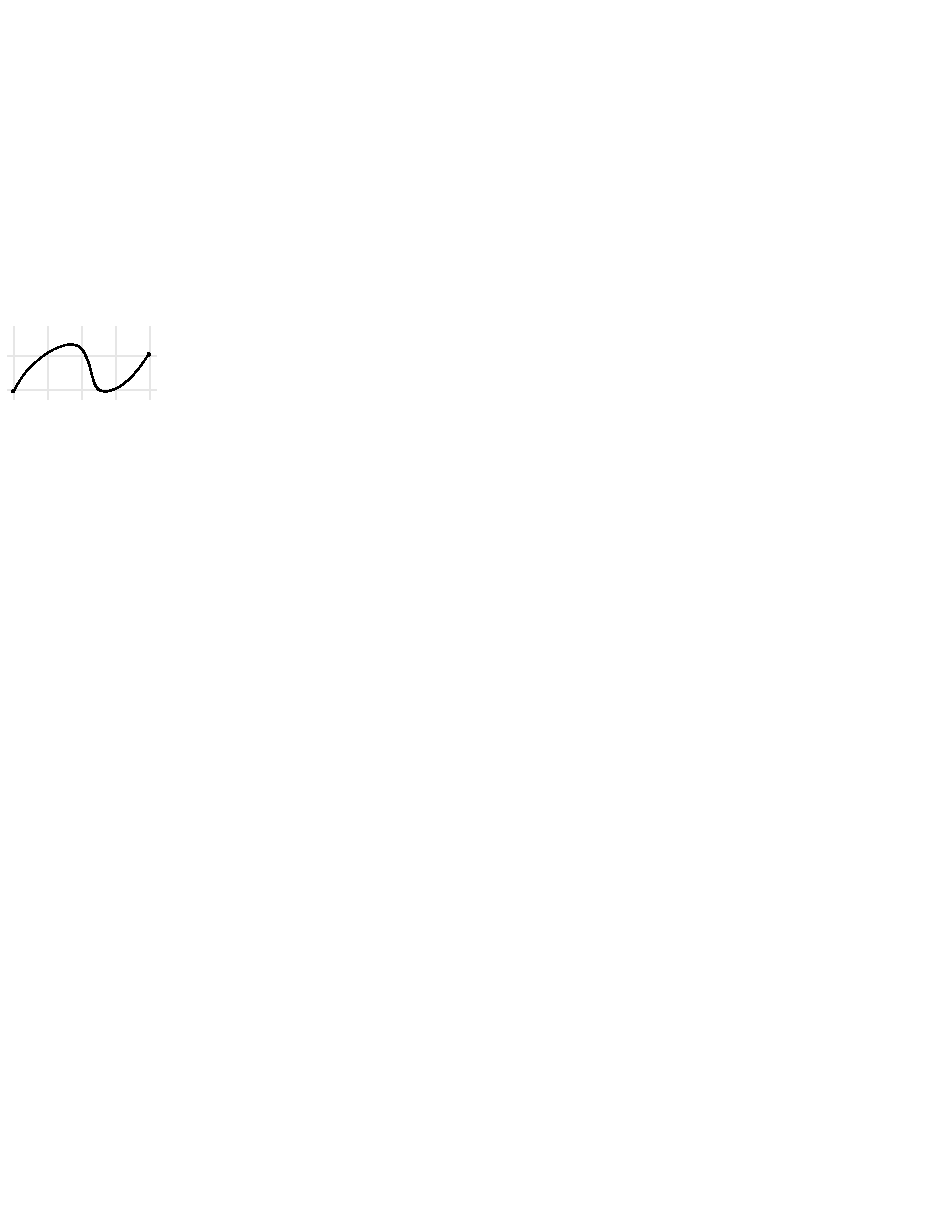
\includegraphics[width=0.3\textwidth]{img/curva_semplice.pdf}
			\caption{Curva semplice.}
		\end{figure}
	
		\item \textcolor{Red3}{\textbf{\underline{Curva non semplice}}} con auto-intersezione, quindi $t_{x} = t_{y}$.
		\begin{figure}[!htp]
			\centering
			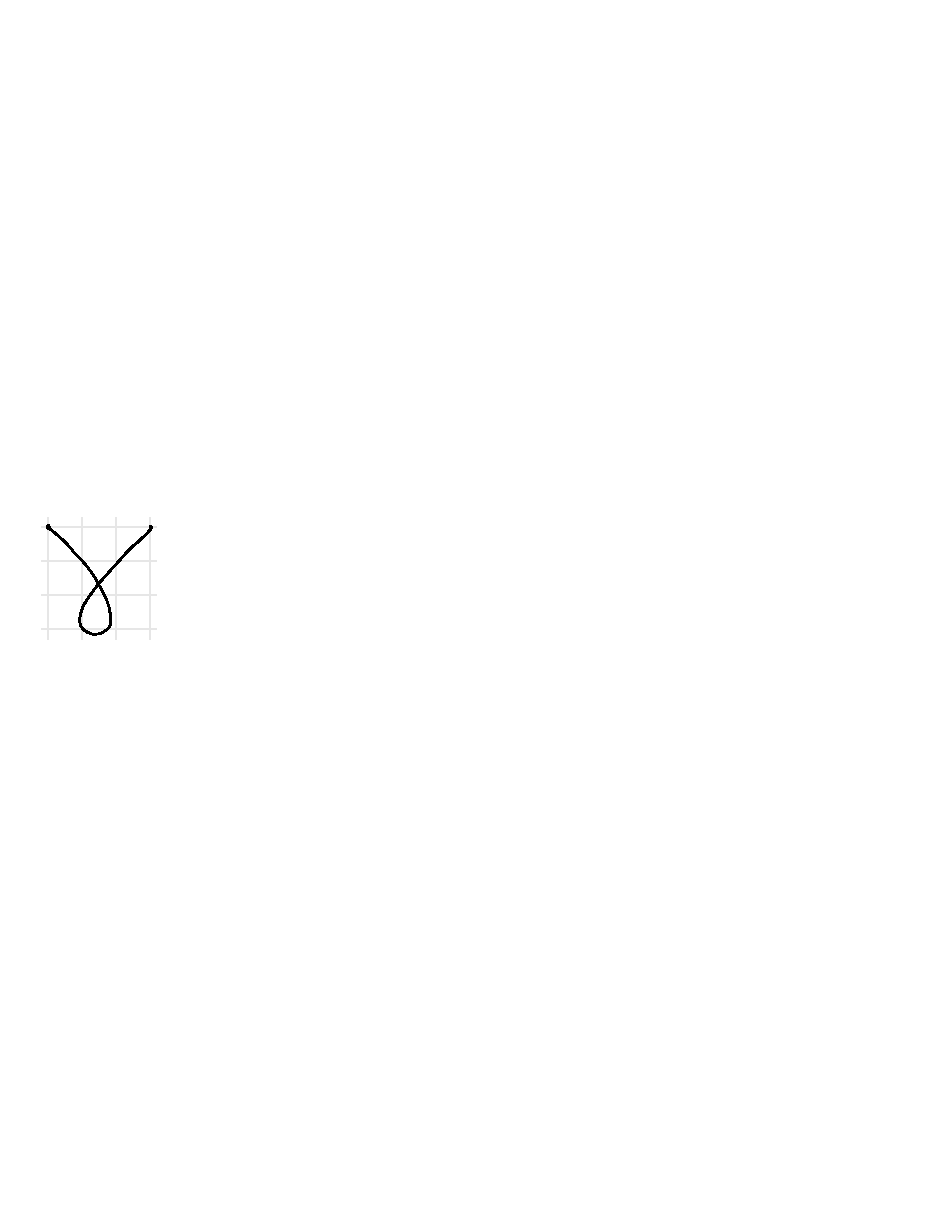
\includegraphics[width=0.2\textwidth]{img/curva_non_semplice.pdf}
			\caption{Curva non semplice.}
		\end{figure}
	
		\item \textcolor{Red3}{\textbf{\underline{Curva chiusa}}} con l'intervallo $I = \left[a,b\right]$ e $\gamma\left(a\right) = \gamma\left(b\right)$. Questa curva è ancora chiamata \textcolor{Red3}{\textbf{semplice}} perché escludendo il caso agli estremi, la curva rimane semplice.
		\begin{figure}[!htp]
			\centering
			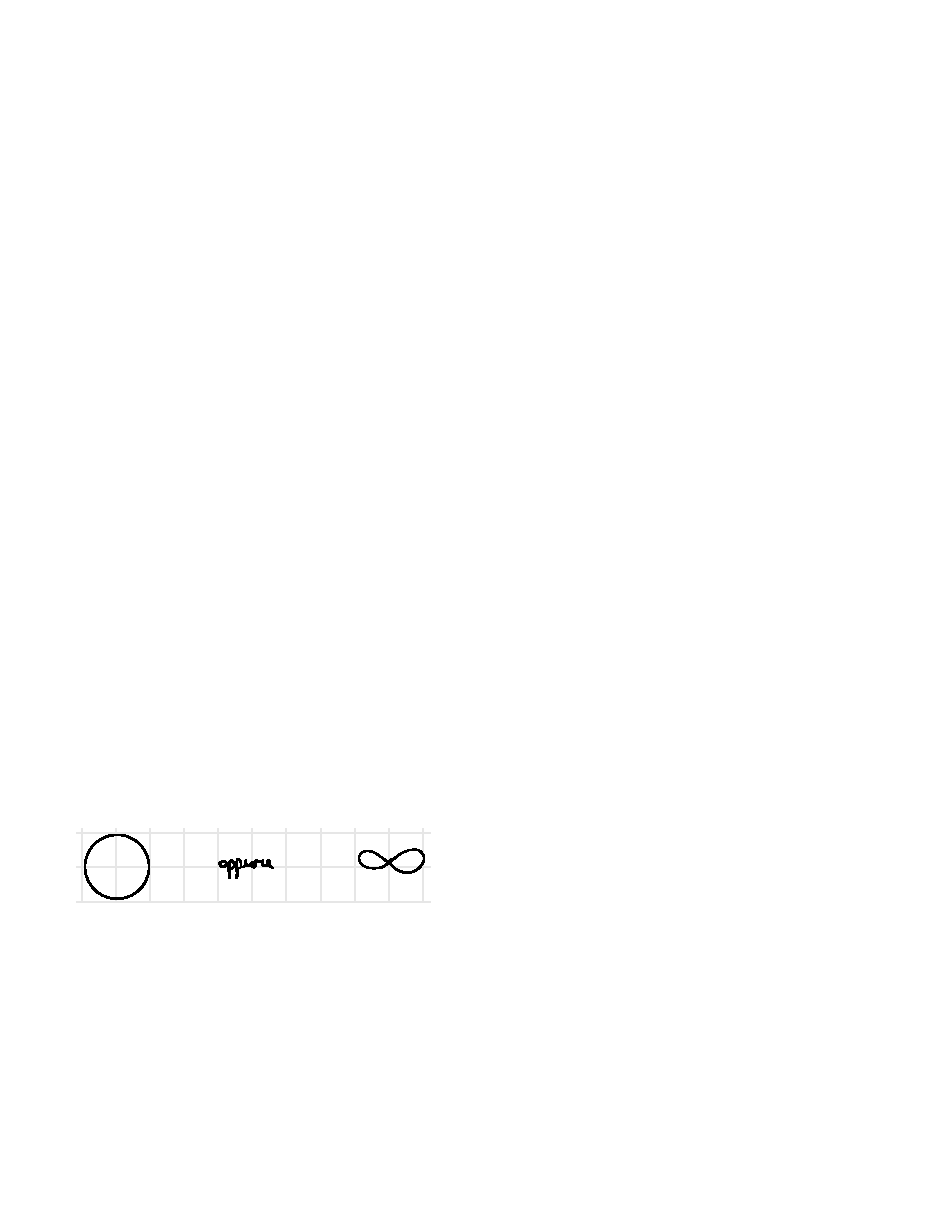
\includegraphics[width=0.5\textwidth]{img/curva_chiusa.pdf}
			\caption{Curva chiusa.}
		\end{figure}
	\end{itemize}
	
	\newpage
	
	\subsubsection[Esempio 1]{\textcolor{Green4}{Esempio 1}}
	
	Data la curva:
	
	\begin{equation*}
		\begin{array}{llll}
			\gamma:	& \left[0,2\pi\right]	& \longrightarrow	& \mathbb{R}^{2} \\
			&&& \\
					& t						& \longmapsto		& \left(\cos\left(t\right), 2 \sin\left(t\right)\right)
		\end{array}
	\end{equation*}
	
	\noindent
	Si ricavano le equazioni parametriche:
	
	\begin{equation*}
		\begin{cases}
			x = \cos\left(t\right) \\
			\\
			y = 2\sin\left(t\right)
		\end{cases}
		\longrightarrow
		\begin{cases}
			x = \cos\left(t\right) \\
			\\
			\dfrac{y}{2} = \sin\left(t\right)
		\end{cases}
	\end{equation*}

	\noindent
	Esiste una relazione tra $\sin$ e $\cos$:
	
	\begin{equation*}
		x^{2} + \dfrac{y^{2}}{4} = \cos^{2}\left(t\right) + \sin^{2}\left(t\right) = 1
	\end{equation*}

	\noindent
	La quale rappresenta l'equazione di un'ellisse di centro $\left(0,0\right)$ e semiassi $a = 1, b = 2$.
	
	\begin{figure}[!htp]
		\centering
		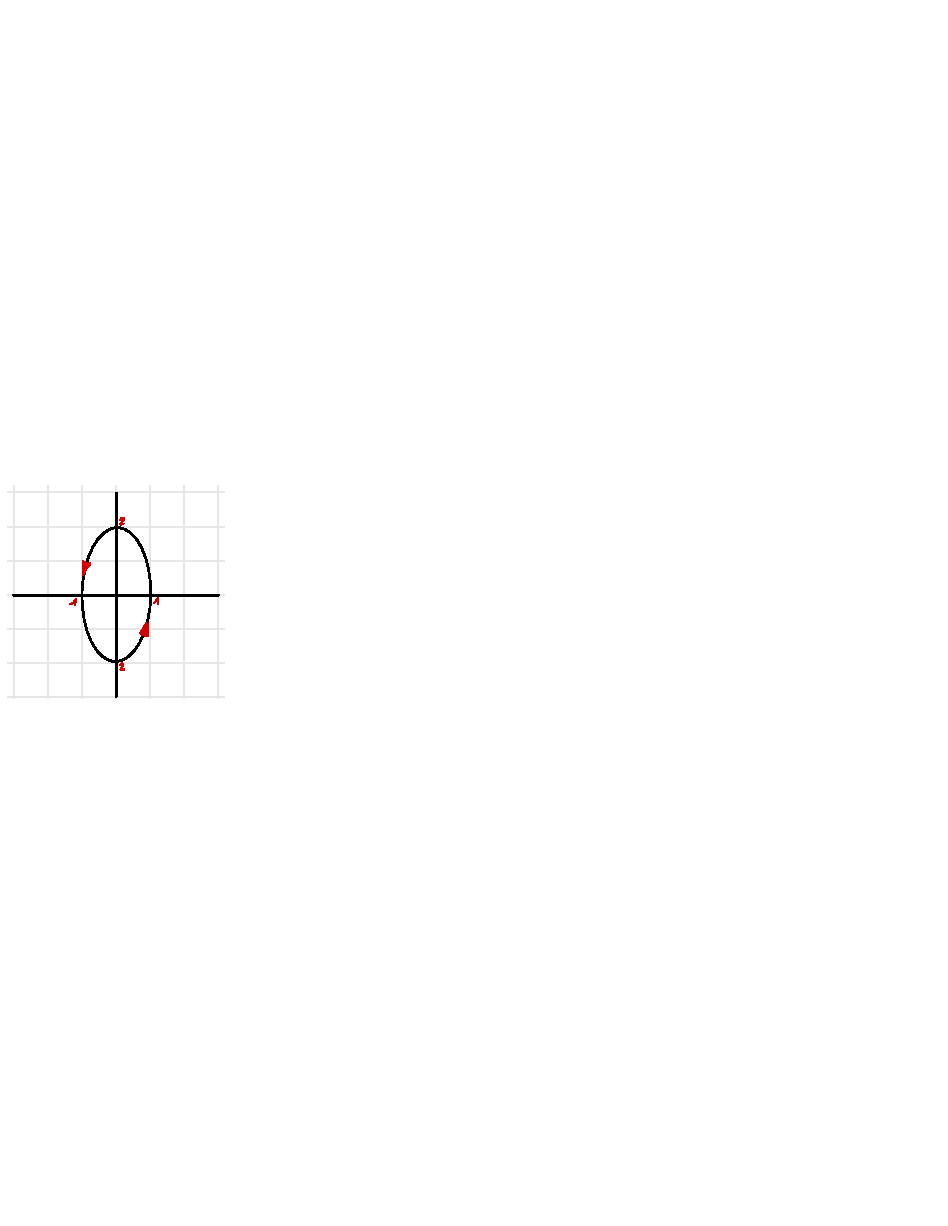
\includegraphics[width=0.6\textwidth]{img/curva_chiusa_semplice_ex1.pdf}
		\caption{Grafico della curva chiusa - semplice.}
	\end{figure}

	\newpage
	
	\subsubsection[Esempio 2]{\textcolor{Green4}{Esempio 2}}
	
	Data la curva:
	
	\begin{equation*}
		\begin{array}{llll}
			\gamma:	& \left[0,\dfrac{\pi}{2}\right]	& \longrightarrow	& \mathbb{R}^{2} \\
			&&& \\
			& t						& \longmapsto		& \left(1 + \cos\left(t\right), \sin\left(t\right)\right)
		\end{array}
	\end{equation*}
	
	\noindent
	Si ricavano le equazioni parametriche:
	
	\begin{equation*}
		\begin{cases}
			x = 1 + \cos\left(t\right) \\
			\\
			y = \sin\left(t\right)
		\end{cases}
		\longrightarrow
		\begin{cases}
			x - 1 = \cos\left(t\right) \\
			\\
			y = \sin\left(t\right)
		\end{cases}
	\end{equation*}
	
	\noindent
	Esiste una relazione tra $\sin$ e $\cos$:
	
	\begin{equation*}
		\left(x-1\right)^{2} + y^{2} = \cos^{2}\left(t\right) + \sin^{2}\left(t\right) = 1
	\end{equation*}

	\noindent
	La quale rappresenta l'equazione di una circonferenza. La rappresentazione grafica è solamente $\frac{1}{4}$ poiché $\frac{\pi}{2}$.
	
	\begin{figure}[!htp]
		\centering
		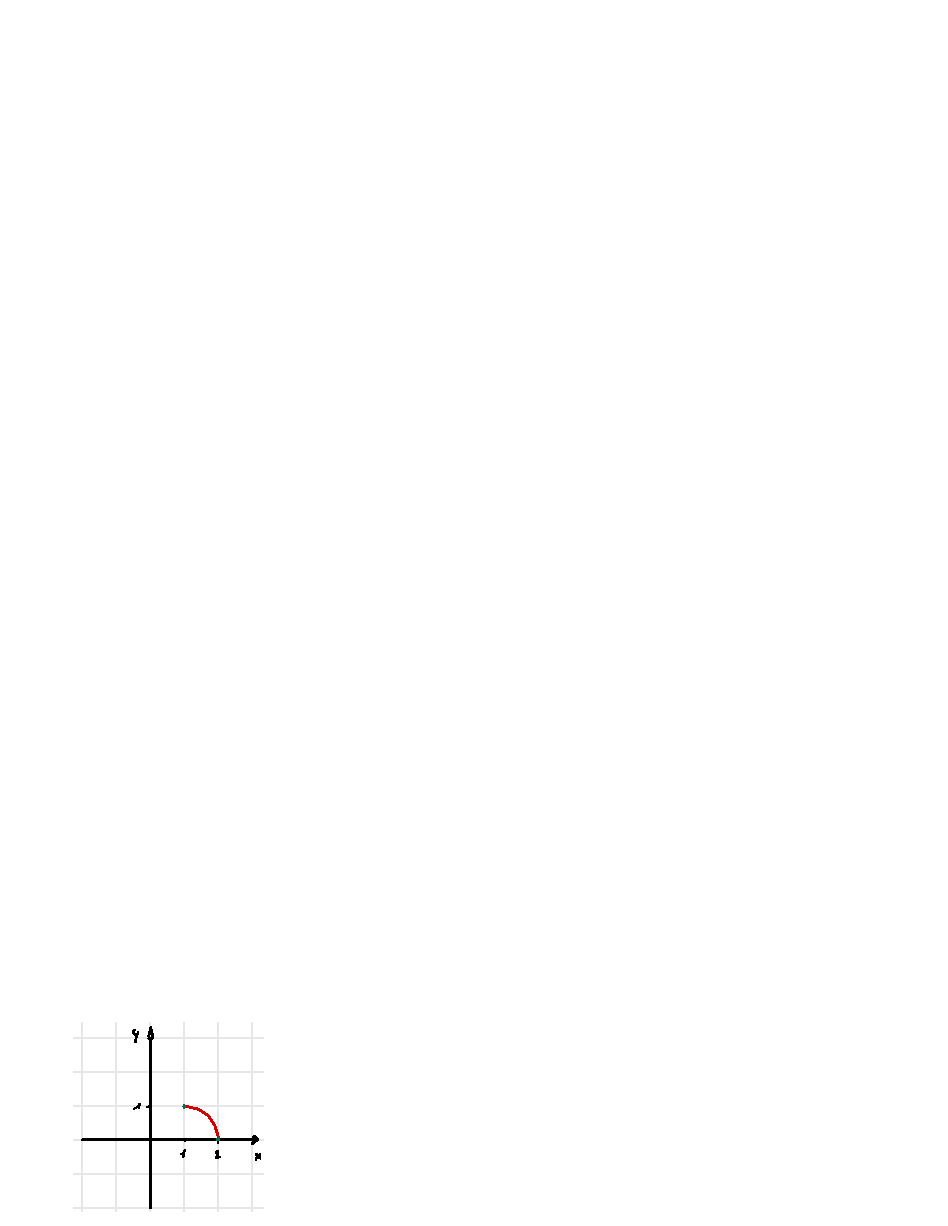
\includegraphics[width=0.6\textwidth]{img/curva_semplice_ex1.pdf}
		\caption{Grafico della curva semplice, ma non chiusa.}
	\end{figure}

	\newpage
	
	\subsubsection[Esempio 3]{\textcolor{Green4}{Esempio 3}}
	
	Data la curva:
	
	\begin{equation*}
		\begin{array}{llll}
			\gamma:	& \mathbb{R}	& \longrightarrow	& \mathbb{R}^{2} \\
			&&& \\
			& t						& \longmapsto		& \left(t^{2}, t^{3} - t\right)
		\end{array}
	\end{equation*}

	\noindent
	La definizione non rappresenta una \textbf{curva semplice} poiché viene violata la proprietà di iniettività, ovvero prendendo due parametri diversi si ha lo stesso risultato. Per esempio:
	
	\begin{equation*}
		\gamma\left(-1\right) = \gamma\left(1\right) = \gamma\left(1,0\right)
	\end{equation*}

	\begin{figure}[!htp]
		\centering
		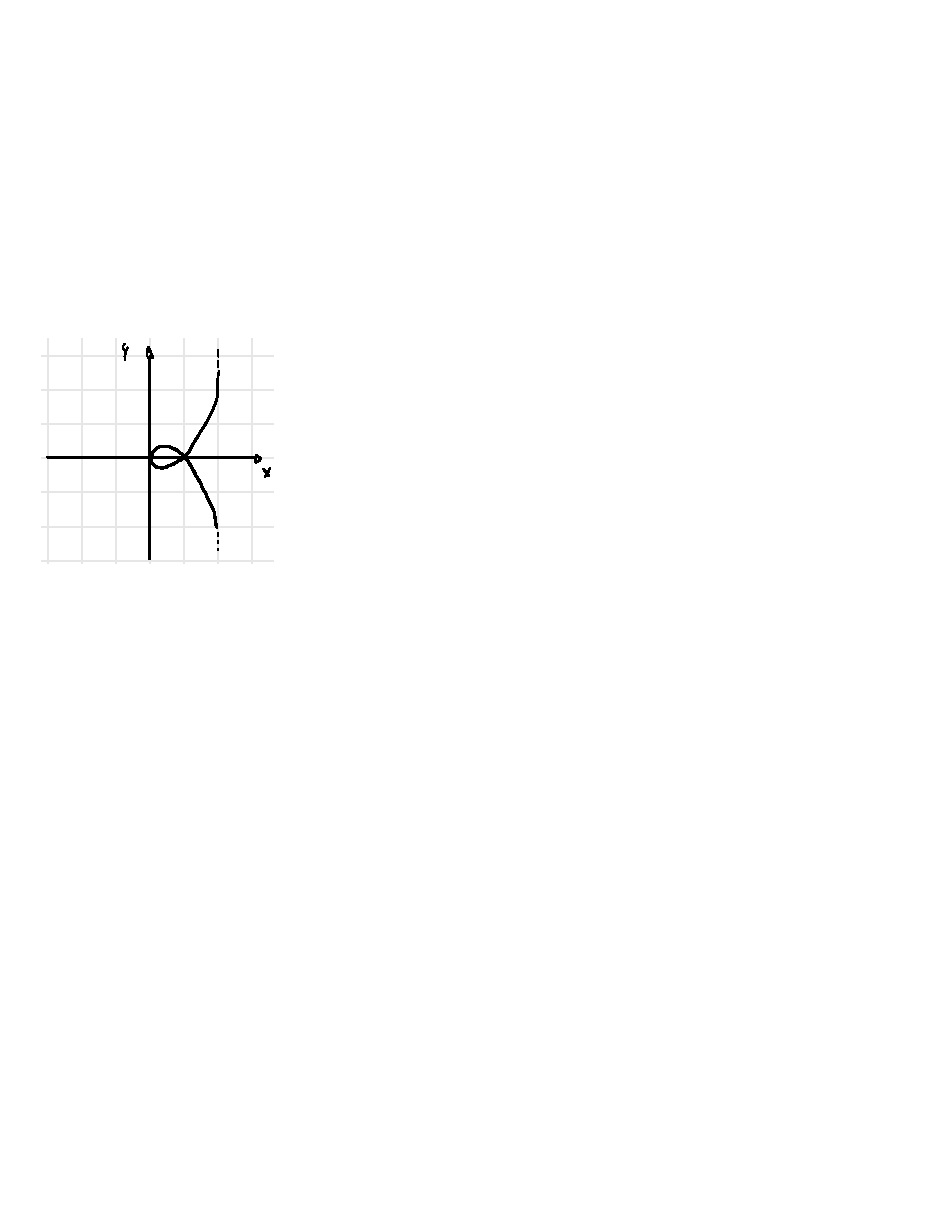
\includegraphics[width=0.6\textwidth]{img/nessuna_curva.pdf}
		\caption{Grafico della curva non semplice e non chiusa}
	\end{figure}

	\newpage
	
	\subsection{Parametrizzazioni notevoli (1° tecnica)}
	
	Alcuni esercizi chiedono di inserire una parametrizzazione.\newline
	
	\noindent
	Per esempio, il \textbf{caso più semplice è un} \textcolor{Red3}{\textbf{\underline{segmento}}}:
	
	\begin{figure}[!htp]
		\centering
		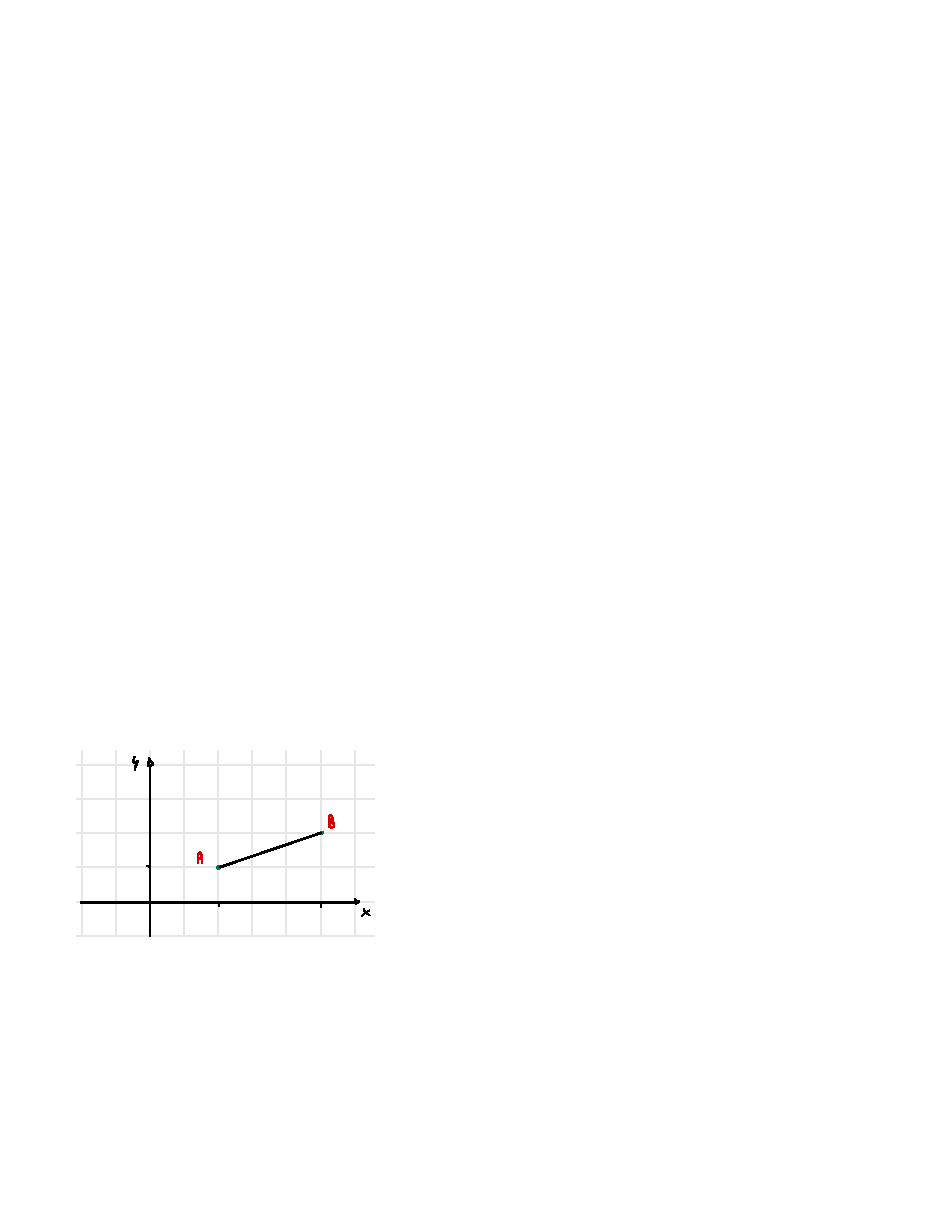
\includegraphics[width=0.5\textwidth]{img/parametrizzazioni_notevoli_segmento.pdf}
	\end{figure}

	\noindent
	Le coordinate dei punti sono:
	
	\begin{equation*}
		\begin{array}{lll}
			A & = & \left(2,1\right) \\
			B & = & \left(5,2\right)
		\end{array}
	\end{equation*}

	\noindent
	Il calcolo di una parametrizzazione prevede di \textcolor{Red3}{\textbf{\underline{definire il vettore che dà la}}} \textcolor{Red3}{\textbf{\underline{direzione della retta}}}. Quindi, nel caso dei segmenti:
	
	\begin{equation*}
		\overrightarrow{V} = B - A = \left(5,2\right) - \left(2,1\right) = \left(3,1\right)
	\end{equation*}

	\noindent
	Una possibile parametrizzazione:
	
	\begin{equation*}
		\gamma\left(t\right) = A + t\overrightarrow{V} \hspace{2em} \text{con } t = \left[0,1\right]
	\end{equation*}

	\noindent
	Il valore $1$ all'interno della definizione della $t$ indica \dquotes{la destinazione}, ovvero le coordinate di destinazione. Quindi, con il valore $1$ si arriva fino alla fine del segmento, mentre con $\frac{1}{2}$ a metà, con $\frac{1}{4}$ a metà della metà e così via.
	
	\begin{equation*}
		\gamma\left(t\right) = A + t\overrightarrow{V} = \left(2,1\right) + t\left(3,1\right) = \left(2 + 3t, 1 + t\right)
	\end{equation*}

	\noindent
	Quindi, una parametrizzazione potrebbe essere:
	
	\begin{equation*}
		\begin{array}{llll}
			\gamma: & \left[0,1\right] & \longrightarrow & \mathbb{R}^{2} \\
			&&& \\
			& t & \longmapsto & \left(2 + 3t, 1 + t\right)
		\end{array}
	\end{equation*}

	\newpage

	\noindent
	\textcolor{Red3}{\textbf{\underline{\emph{Variante dell'esercizio}}}}\newline
	
	\noindent
	Una variante dell'esercizio potrebbe essere la seguente. Data una parametrizzazione della retta:
	
	\begin{equation*}
		\begin{array}{llll}
			\gamma: & \mathbb{R} & \longrightarrow & \mathbb{R}^{2} \\
			&&& \\
			& t & \longmapsto & \left(2 + 3t, 1 + t\right)
		\end{array}
	\end{equation*}

	\noindent
	È possibile ricostruire l'equazione cartesiana?\newline
	
	\noindent
	Per ottenere l'equazione si esplicita la $t$ nelle equazioni parametriche:
	
	\begin{equation*}
		\begin{cases}
			x = 2 + 3t \\
			\\
			y = 1 + t
		\end{cases}
		\longrightarrow
		\begin{cases}
			t = \dfrac{x - 2}{3} \\
			\\
			y = 1 + \dfrac{x - 2}{3}
		\end{cases}
	\end{equation*}

	\noindent
	Quindi, l'equazione che si ottiene:
	
	\begin{equation*}
		y - 1 = \dfrac{1}{3}\left(x - 2\right)
	\end{equation*}

	\noindent
	Che rappresenta l'equazione della retta nel fascio proprio di centro $A$.
	
	\newpage
	
	\subsection{Parametrizzazioni notevoli (2° tecnica)}
	
	Dato il grafico di una funzione $f$:
	
	\begin{equation*}
		\begin{array}{llll}
			f: & I & \longrightarrow & \mathbb{R} \\
			   & x & \longmapsto     & f\left(x\right)
		\end{array}
	\end{equation*}

	\noindent
	La parametrizzazione corrisponde a:
	
	\begin{equation*}
		\begin{array}{llll}
			f: & I & \longrightarrow & \mathbb{R}^{2} \\
			& t & \longmapsto     & \left(t, f\left(t\right)\right)
		\end{array}
	\end{equation*}

	\noindent
	\textcolor{Green4}{\textbf{Per esempio}}, la parametrizzazione di un \textcolor{Red3}{\textbf{\underline{arco di parabola}}}:
	
	\begin{equation*}
		y = 1 - x^{2} \hspace{2em} \text{con } x \in \left[0,2\right]
	\end{equation*}

	\noindent
	Si ottiene:
	
	\begin{equation*}
		\begin{array}{llll}
			\sigma: & \left[0,2\right] & \longrightarrow & \mathbb{R}^{2} \\
			& t & \longmapsto     & \left(t, 1-t^{2}\right)
		\end{array}
	\end{equation*}

	\begin{figure}[!htp]
		\centering
		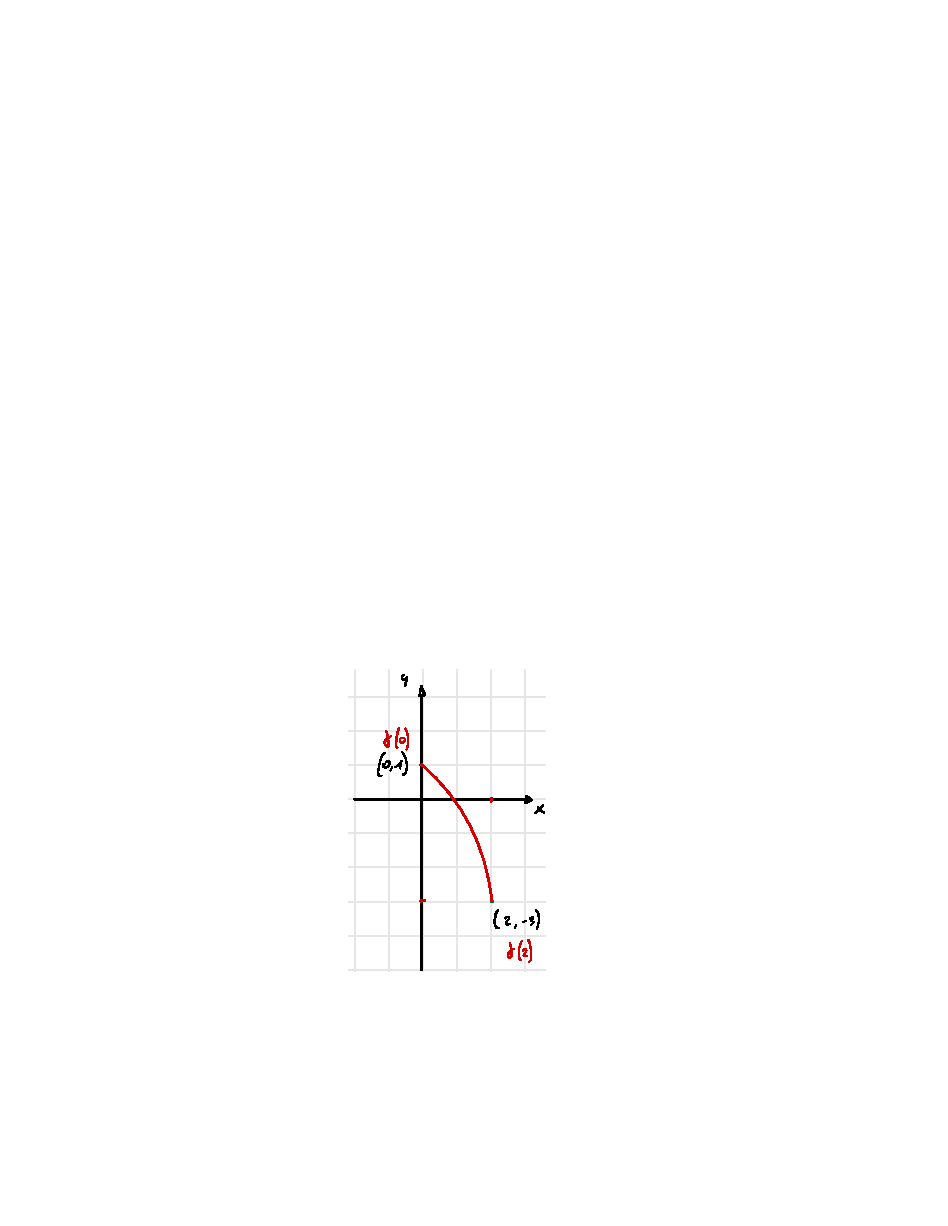
\includegraphics[width=0.4\textwidth]{img/parametrizzazioni_notevoli_parabola}
	\end{figure}

	\newpage
	
	\subsection{Parametrizzazioni notevoli (casi complessi)}
	
	Esistono delle parametrizzazioni notevoli complesse, come quella delle \textcolor{Red3}{\textbf{\underline{canoniche}}}.\newline
	
	\noindent
	Un'altra parametrizzazione complessa è quella della \textcolor{Red3}{\textbf{\underline{ellisse}}} di centro $c\left(x_{c}, y_{c}\right)$ e semiassi $a,b$:
	
	\begin{equation*}
		\begin{array}{llll}
			\gamma: & \left[0,2\pi\right] & \longrightarrow & \mathbb{R}^{2} \\
			&&& \\
					& t					  & \longmapsto		& \left(x_{c} + a \cos\left(t\right), y_{c} + b \sin\left(t\right)\right)
		\end{array}
	\end{equation*}

	\noindent
	E ancora, un'altra parametrizzazione complessa è la \textcolor{Red3}{\textbf{\underline{iperbole equilatera}}}:
	
	\begin{equation*}
		x^{2} - y^{2} - 1 = 0
	\end{equation*}

	\noindent
	Con una parametrizzazione $\boldsymbol{x > 0}$:
	
	\begin{equation*}
		\begin{array}{llll}
			\gamma: & \mathbb{R} & \longrightarrow & \mathbb{R}^{2} \\
					& t			 & \longmapsto	   & \left(\cosh\left(t\right), \sinh\left(t\right)\right)
		\end{array}
	\end{equation*}

	\noindent
	Invece, con una parametrizzazione $\boldsymbol{x < 0}$:
	
	\begin{equation*}
		\begin{array}{llll}
			\gamma: & \mathbb{R} & \longrightarrow & \mathbb{R}^{2} \\
					& t			 & \longmapsto	   & \left(- \cosh\left(t\right), \sinh\left(t\right)\right)
		\end{array}
	\end{equation*}

	\noindent
	Si ricorda inoltre che:
	
	\begin{equation*}
		\begin{array}{lll}
			\text{Coseno iperbolico:}	& \cosh\left(t\right) =	& \dfrac{e^{t} + e^{-t}}{2} \\
			\\
			\text{Seno iperbolico:}		& \sinh\left(t\right) =	& \dfrac{e^{t} - e^{-t}}{2}
		\end{array}
	\end{equation*}

	\begin{figure}[!htp]
		\centering
		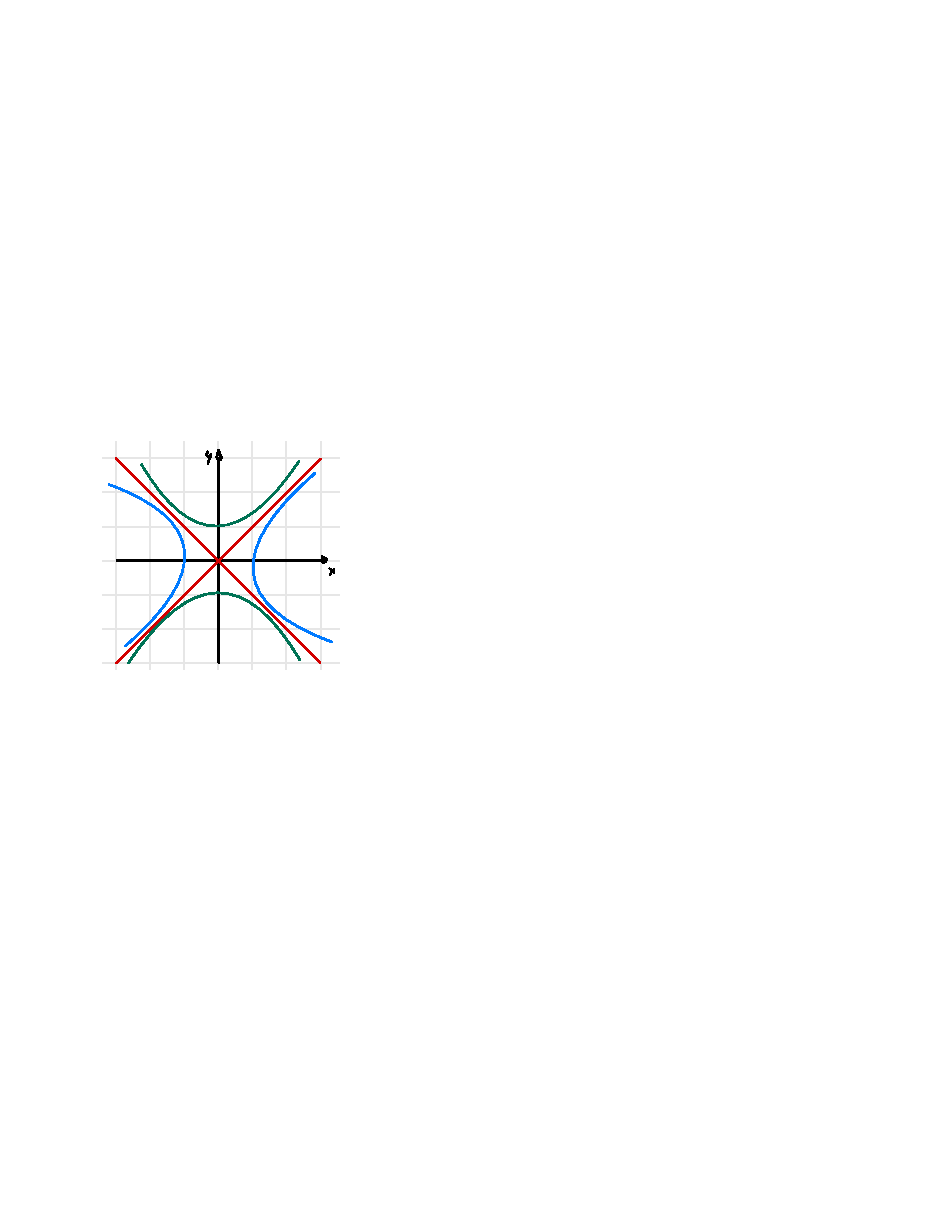
\includegraphics[width=0.4\textwidth]{img/iperbole_equilatera.pdf}
		\caption{In rosso gli asindoti, in verde l'iperbole $x^{2} - y^{2} + 1 = 0$, in blu l'iperbole $x^{2} - y^{2} - 1 = 0$.}
	\end{figure}

	\noindent
	Infine, la parametrizzazione di un'\textcolor{Red3}{\textbf{\underline{iperbole normale}}}:
	
	\begin{equation*}
		\sigma\left(t\right) = \left(x_{c} \pm a \cdot \cosh\left(t\right), y_{c} + b \cdot \sinh\left(t\right)\right) \xrightarrow{parametrizza} \dfrac{\left(x - x_{c}\right)^{2}}{a^{2}} - \dfrac{\left(y - y_{c}\right)^{2}}{b^{2}} = 1
	\end{equation*}

	\newpage
	
	\subsection{Derivata di una curva}
	
	Una \textcolor{Red3}{\textbf{\underline{curva}}} è \textcolor{Red3}{\textbf{\underline{derivabile}}} in $I$ se tutte le sue componenti sono derivabili in $I$ e in tal caso:
	
	\begin{equation*}
		\gamma'\left(t\right) = \left(\gamma_{1}'\left(t\right), \gamma_{2}'\left(t\right), ..., \gamma_{n}'\left(t\right)\right)
	\end{equation*}
	
	\noindent
	Ogni $\gamma'$ viene definita come:
	
	\begin{equation*}
		\gamma'\left(t\right) = \lim_{h \rightarrow 0} \dfrac{r\left(t+h\right) - \gamma\left(t\right)}{h}
	\end{equation*}

	\begin{figure}[!htp]
		\centering
		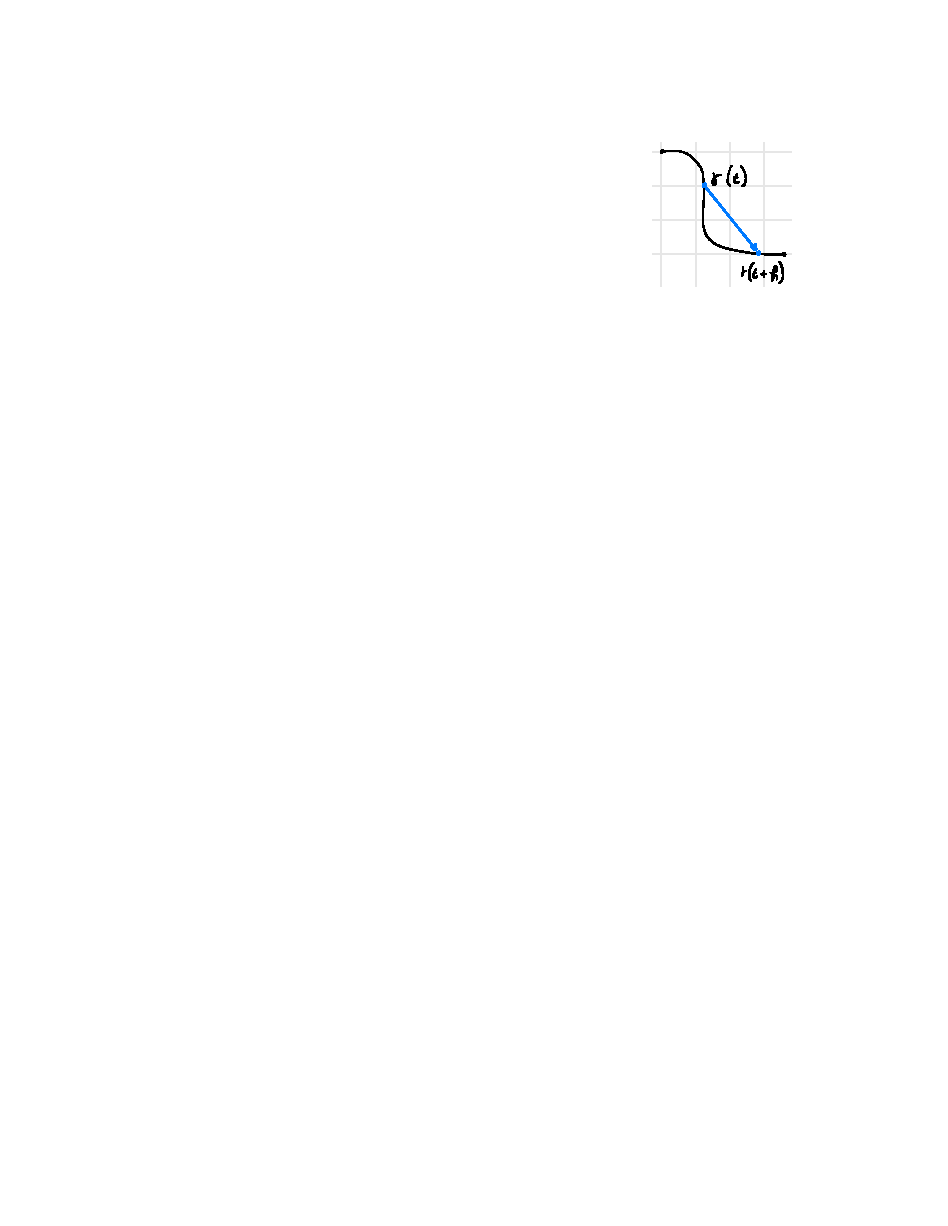
\includegraphics[width=0.3\textwidth]{img/derivata_curva.pdf}
		\caption{Rappresentazione grafica della derivata.}
	\end{figure}

	\noindent
	Se $\gamma'\left(t_{0}\right) \ne \overrightarrow{0}$ (\textcolor{Red3}{\textbf{\underline{non è un vettore nullo}}}) allora una parametrizzazione della retta tangente al sostegno di $\gamma$ nel punto $\gamma\left(t_{0}\right)$:
	
	\begin{equation*}
		r\left(t\right) = \gamma\left(t_{0}\right) + t \cdot \gamma'\left(t_{0}\right)
	\end{equation*}

	\noindent
	Dove $\gamma\left(t_{0}\right)$ indica il punto iniziale e $\gamma'\left(t_{0}\right)$ indica il vettore che dà la direzione.
	
	\begin{figure}[!htp]
		\centering
		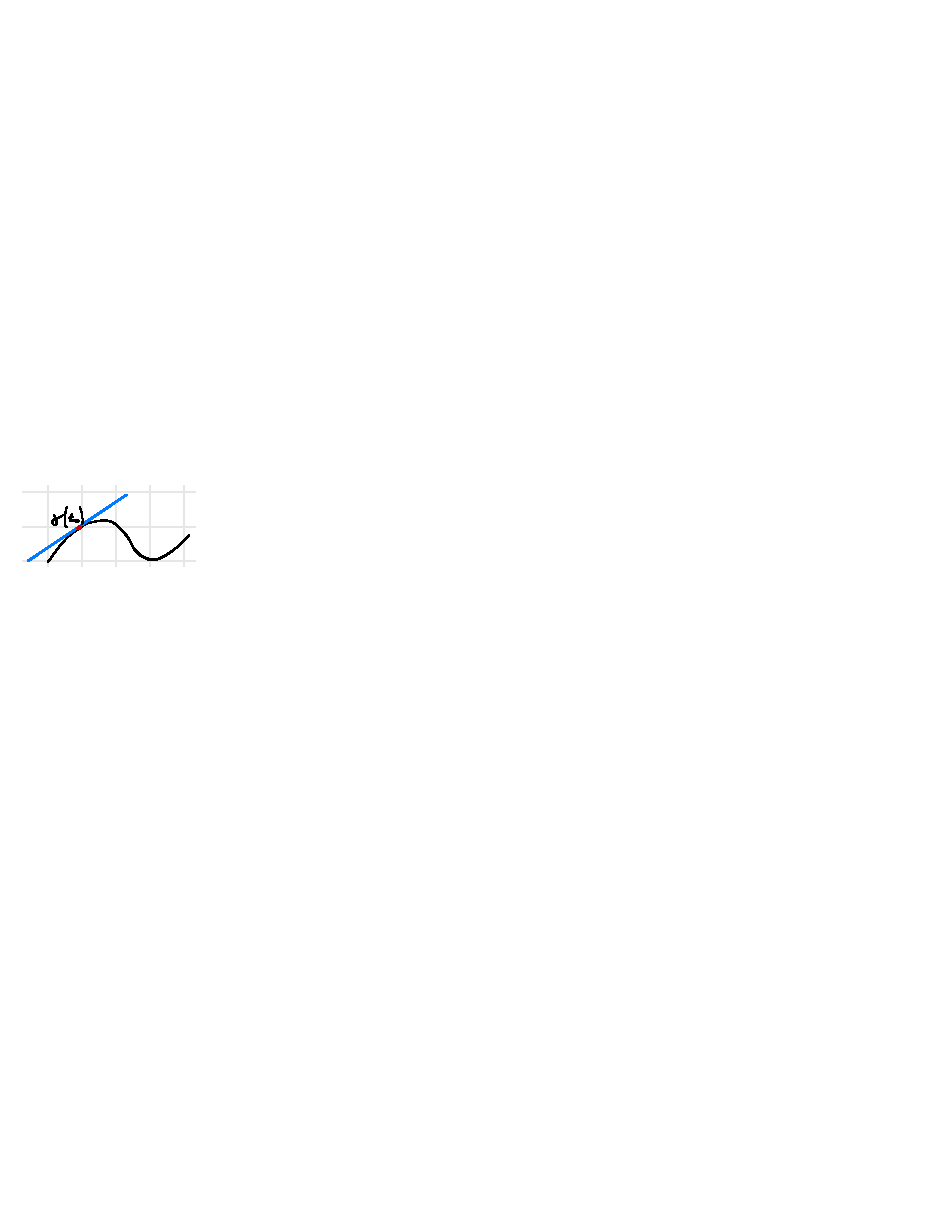
\includegraphics[width=0.5\textwidth]{img/derivata_curva2.pdf}
		\caption{Parametrizzazione retta tangente al sostegno di $\gamma$ nel punto $\gamma\left(t_{0}\right)$.}
	\end{figure}

	\newpage
	
	\subsubsection[Esercizio guidato]{\textcolor{Green4}{Esercizio guidato}}
	
	Trovare l'equazione della retta tangente al sostegno della curva:
	
	\begin{equation*}
		\begin{array}{llll}
			\gamma:	& \left(-1,\infty\right) & \longrightarrow & \mathbb{R}^{3} \\
					& t						 & \longmapsto     & \left(e^{t}, \ln\left(t+1\right), t\right)
		\end{array}
	\end{equation*}

	\noindent
	Nel suo punto di coordinate $\left(0,0,1\right)$.\newline
	
	\noindent
	\textcolor{Red3}{\textbf{\underline{Passo 1}}}\newline

	\noindent
	Trovare $t_{0 \in \left(-1, \infty\right)}$ tale che $\gamma\left(t_{0}\right) = \left(1,0,0\right)$:
	
	\begin{equation*}
		\begin{cases}
			e^{t} = 1 \\
			\ln\left(t+1\right) = 0 \xrightarrow{soluzione} t_{0} = 0 \in \mathbb{R} \\
			t = 0
		\end{cases}
	\end{equation*}

	\noindent
	\textcolor{Red3}{\textbf{\underline{Passo 2}}}\newline
	
	\noindent
	Calcolare il vettore tangente (derivata delle componenti):
	
	\begin{equation*}
		\gamma'\left(t_{0}\right) = \left(\gamma_{1}'\left(t_{0}\right), \gamma_{2}'\left(t_{0}\right), \gamma_{3}'\left(t_{0}\right)\right) = \left(1,1,1\right)
	\end{equation*}

	\noindent
	\textcolor{Red3}{\textbf{\underline{Passo 3}}}\newline
	
	\noindent
	Parametrizzazione della retta tangente:
	
	\begin{equation*}
		r\left(t\right) = \left(1,0,0\right) + t\left(1,1,1\right) = \left(1+t, t, t\right) \hspace{2em} \text{con } t\in\mathbb{R}
	\end{equation*}

	\noindent
	Le equazioni parametriche della retta tangente:
	
	\begin{equation*}
		\begin{cases}
			x = 1+t \\
			y = t \\
			z = t
		\end{cases}
	\end{equation*}

	\newpage
	
	\subsection{Insiemi connessi per archi}
	
	Dato un insieme $D \subseteq \mathbb{R}^{n}$ si dice che è \textcolor{Red3}{\textbf{\underline{connesso per archi}}} se presi due punti qualunque $x,y$ in $D$ esiste un cammino (arco) in $D$ che ha per estremi $x$ e $y$. Si noti bene che in $\mathbb{R}$ solo gli intervalli (aperti o chiusi) sono connessi.
	
	\begin{figure}[!htp]
		\centering
		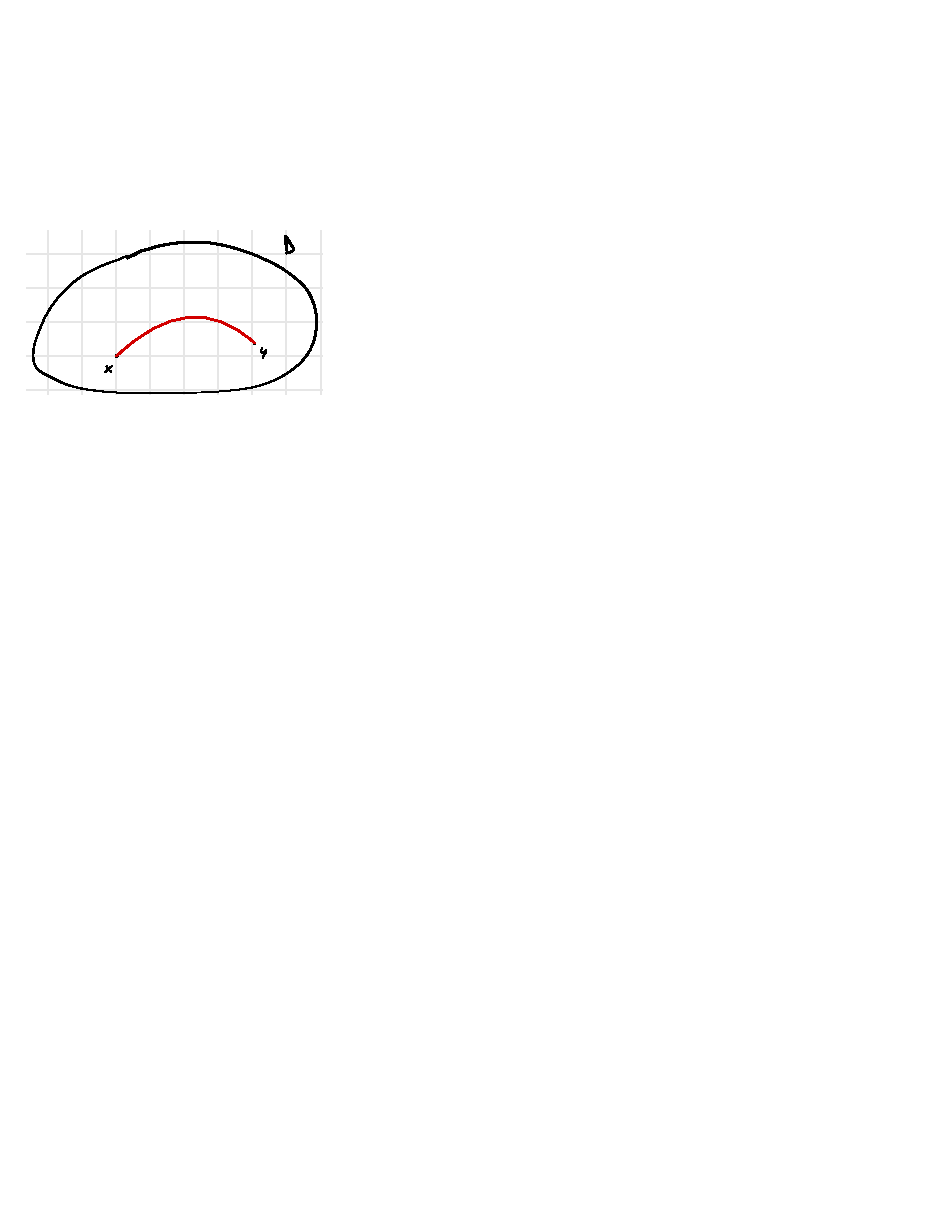
\includegraphics[width=0.4\textwidth]{img/connesso_per_archi1.pdf}
		\caption{Esempio di connessione per archi.}
		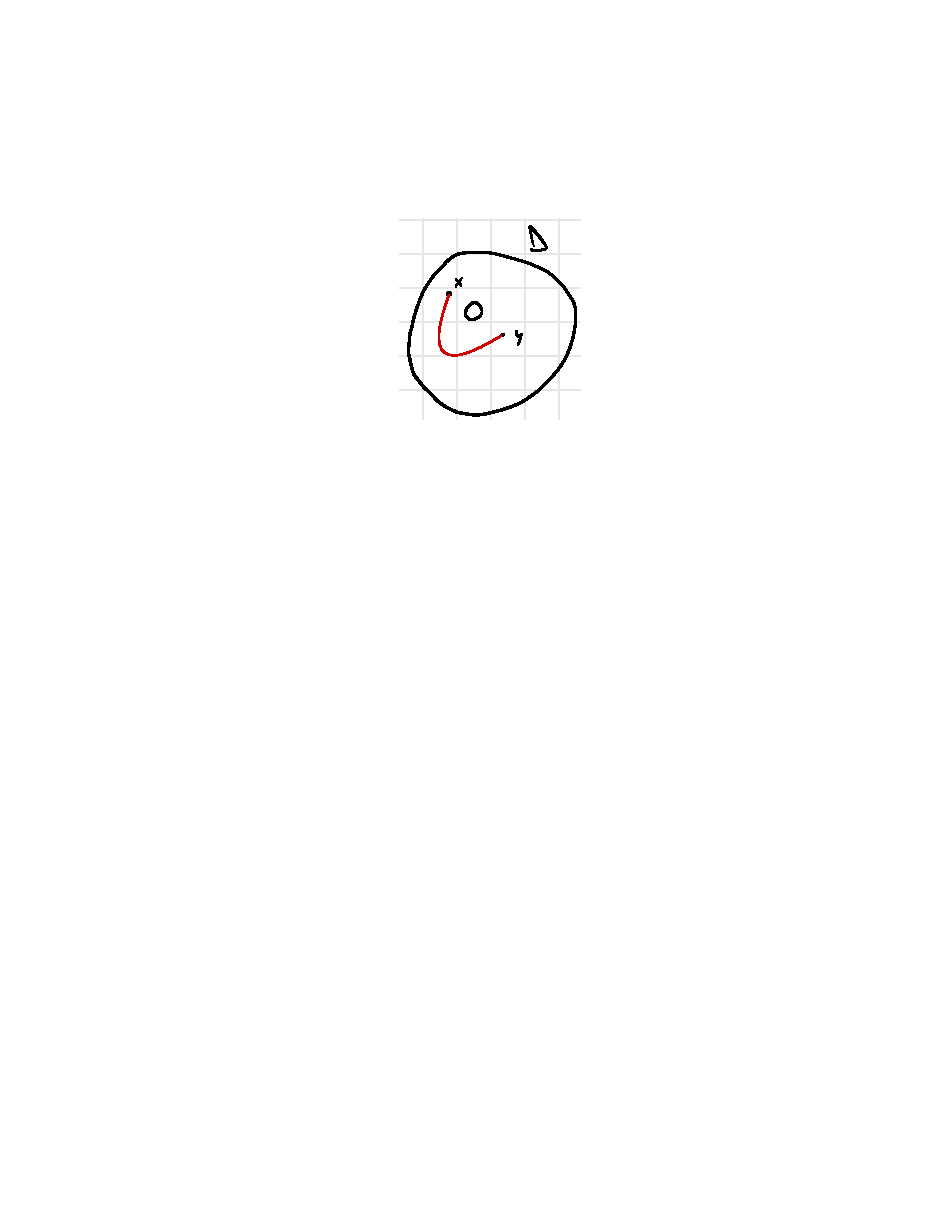
\includegraphics[width=0.4\textwidth]{img/connesso_per_archi2.pdf}
		\caption{Esempio di connessione per archi.}
		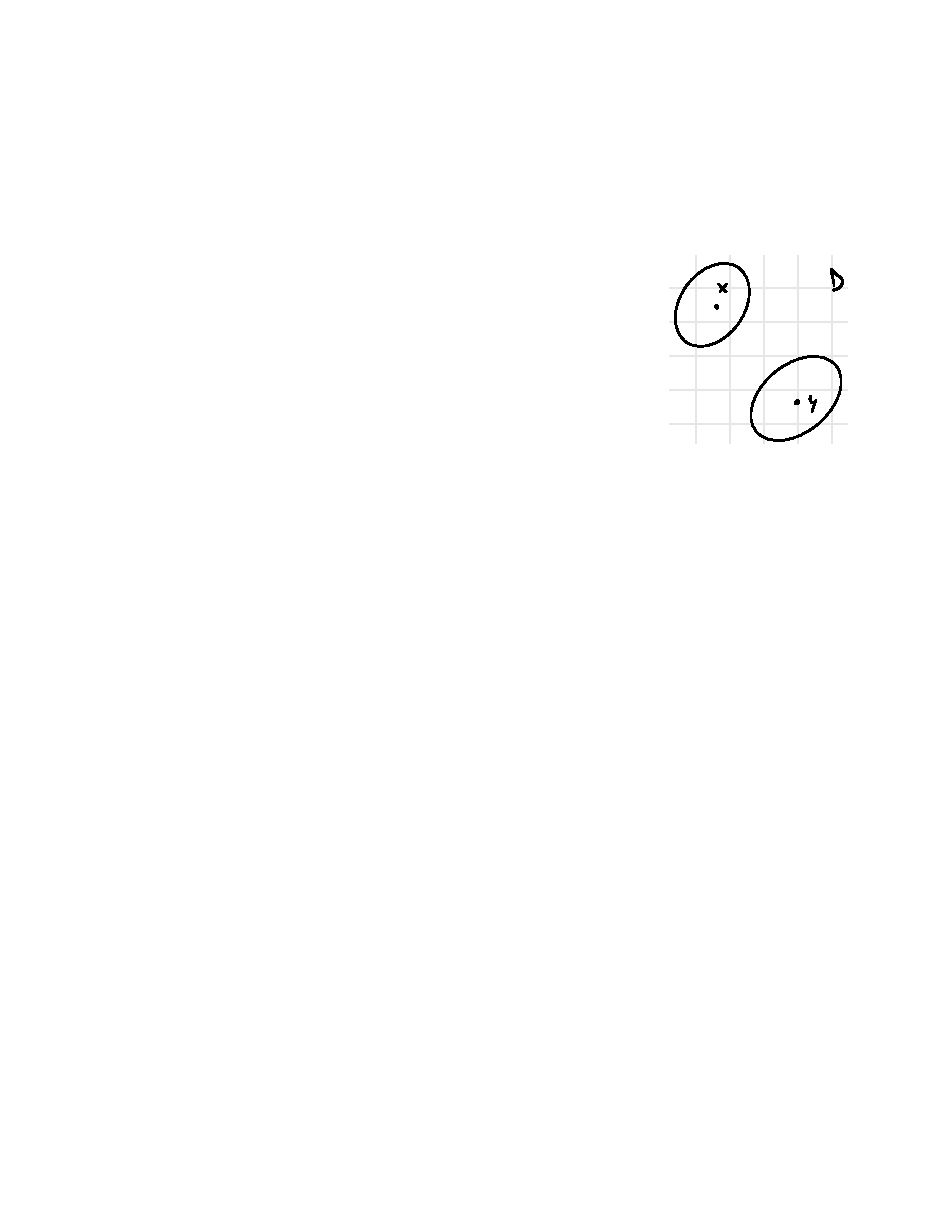
\includegraphics[width=0.4\textwidth]{img/connesso_per_archi3.pdf}
		\caption{Esempio di \textbf{non} connessione per archi.}
	\end{figure}

	\newpage
	
	\subsection{Teorema degli zeri}
	
	Sia $f$ una funzione \textbf{continua} su un insieme $D \subseteq \mathbb{R}^{n}$ \textbf{connesso per archi}.\newline
	Se $x,y$ sono due punti di $D$ tali che $f\left(x\right) > 0$ e $f\left(y\right) < 0$, allora esiste $z \in D$ tale che $f\left(z\right) = 0$.\newline
	
	\noindent
	I requisiti in cui vale il teorema sono quelli della definizione, ovvero la funzione deve essere:
	
	\begin{itemize}
		\item Continua
		\item Connessa per archi
	\end{itemize}

	\newpage
	
	\section{Lezione 12}
	
	\subsection{Derivate parziali}
	
	Dato il grafico:
	
	\begin{figure}[!htp]
		\centering
		\includegraphics[width=0.5\textwidth]{img/derivate_parziali.pdf}
	\end{figure}
	
	\noindent
	Il punto $P$ si muove parallelamente agli assi. La funzione $f$ è definita in un intorno di $\left(x_{0}, y_{0}\right)$:
	
	\begin{equation*}
		x \longrightarrow f\left(x,y\right)
	\end{equation*}

	\noindent
	Indica la restrizione della funzione $f$ alla retta di equazione $y = y_{0}$. Se tale restrizione è derivabile in $x_{0}$, si dice che $f$ ammette \textbf{\underline{derivate parziali rispetto a $\boldsymbol{x}$}} in $\left(x_{0}, y_{0}\right)$.\newline
	
	\noindent
	Quindi, la \textcolor{Red3}{\textbf{\underline{derivata parziale rispetto a $\boldsymbol{x}$}}}:
	
	\begin{equation*}
		\dfrac{\partial f}{\partial x} \left(x_{0}, y_{0}\right) = \lim_{h \rightarrow 0} \dfrac{f\left(x_{0} + h, y_{0}\right) - f\left(x_{0}, y_{0}\right)}{h}
	\end{equation*}

	\noindent
	In modo analogo, si definisce la \textcolor{Red3}{\textbf{\underline{derivata parziale rispetto a $\boldsymbol{y}$}}}:
	
	\begin{equation*}
		\dfrac{\partial f}{\partial y} \left(x_{0}, y_{0}\right) = \lim_{h \rightarrow 0} \dfrac{f\left(x_{0}, y_{0} + h\right) - f\left(x_{0}, y_{0}\right)}{h}
	\end{equation*}

	\newpage

	\subsubsection{Implementazione geometrica con $\boldsymbol{n = 2}$}
	
	Le due derivate parziali sono i coefficienti delle rette tangenti in $\left(x_{0}, y_{0}, f\left(x_{0}, y_{0}\right)\right)$ alle curve ottenute sezionando il grafico di $f$ con i piani $y = y_{0}$ e $x = x_{0}$ rispettivamente.
	
	\begin{figure}[!htp]
		\centering
		\includegraphics[width=0.5\textwidth]{img/interpretazione_geometrica1.pdf}
	\end{figure}
	
	\subsubsection{Implementazione geometrica con $\boldsymbol{n \ge 2}$}
	
	Con la funzione $f$ viene definita in un intorno di $P \in \mathbb{R}^{n}$:
	
	\begin{equation*}
		\dfrac{\partial f}{\partial x_{i}}\left(P\right) = \lim_{h \rightarrow 0} \dfrac{f\left(P + h e_{i}\right) - f\left(P\right)}{h} \hspace{2em} \text{con } e_{i} = \left(0,0,0,0, ..., 1, ..., 0,0,0,0\right)
	\end{equation*}

	\noindent
	Con $1$ che indica la $i$-esima.
	
	\newpage
	
	\subsection{Tecnica risolutiva derivate parziali}
	
	La tecnica di risoluzione delle derivate corrisponde a quella spiegata in Analisi I.
	
	\subsubsection[Esempio 1]{\textcolor{Green4}{Esempio 1}}
	
	Data la funzione:
	
	\begin{equation*}
		f\left(x,y\right) = x^{2} e^{xy}
	\end{equation*}

	\noindent
	Con la $y$ costante:
	
	\begin{equation*}
		\dfrac{\partial f}{\partial x}\left(x,y\right) = 2xe^{xy} + x^{2} e^{xy} y = xe^{xy} \cdot \left(2 + xy\right)
	\end{equation*}

	\noindent
	Con la $x$ costante:
	
	\begin{equation*}
		\dfrac{\partial f}{\partial y}\left(x,y\right) = x^{2} e^{xy} \cdot x = x^{3} e^{xy}
	\end{equation*}

	\subsubsection[Esempio 2]{\textcolor{Green4}{Esempio 2}}
	
	Data la funzione:
	
	\begin{equation*}
		f\left(v,w\right) = \dfrac{w}{v^{2} + w^{2}}
	\end{equation*}
	
	\noindent
	Con la $w$ costante:
	
	\begin{equation*}
		\dfrac{\partial f}{\partial v}\left(v,w\right) = \dfrac{0 - w \cdot 2v}{\left(v^{2} + w^{2}\right)^{2}} = - \dfrac{2 v w}{\left(v^{2} + w^{2}\right)^{2}}
	\end{equation*}
	
	\noindent
	Con la $v$ costante:
	
	\begin{equation*}
		\dfrac{\partial f}{\partial w}\left(v,w\right) = \dfrac{1\left(v^{2} + w^{2}\right) - w \cdot 2w}{\left(v^{2} + w^{2}\right)^{2}} = \dfrac{v^{2} - w^{2}}{\left(v^{2} + w^{2}\right)^{2}}
	\end{equation*}

	\subsubsection[Esempio 3]{\textcolor{Green4}{Esempio 3}}
	
	Data la funzione:
	
	\begin{equation*}
		f\left(x,y,z\right) = xyz
	\end{equation*}

	\noindent
	Con le $y,z$ costanti:
	
	\begin{equation*}
		\dfrac{\partial f}{\partial x}\left(x,y,z\right) = yz
	\end{equation*}

	\noindent
	Con le $x,z$ costanti:
	
	\begin{equation*}
		\dfrac{\partial f}{\partial y}\left(x,y,z\right) = xz
	\end{equation*}

	\noindent
	Con le $x,y$ costanti:
	
	\begin{equation*}
		\dfrac{\partial f}{\partial z}\left(x,y,z\right) = xy
	\end{equation*}

	\newpage
	
	\subsubsection{Esempio 4 da \textcolor{Red3}{esame}}
	
	Calcolare la derivata, se esiste:
	
	\begin{equation*}
		\dfrac{\partial f}{\partial x}\left(0,0\right)
	\end{equation*}

	\noindent
	Data la funzione:
	
	\begin{equation*}
		f\left(x,y\right) = y \sqrt[3]{x}
	\end{equation*}

	\noindent
	Applicando le regole classiche, come negli esercizi precedenti:
	
	\begin{equation*}
		\dfrac{\partial f}{\partial x}\left(x,y\right) = y \cdot \dfrac{1}{3 \sqrt[3]{x^{2}}}
	\end{equation*}

	\noindent
	È evidente che \textbf{non è definita nel punto} $\left(0,0\right)$.\newline
	
	\noindent
	Quindi, è necessaria la definizione di derivata parziale:
	
	\begin{equation*}
		\dfrac{\partial f}{\partial x}\left(0,0\right) = \lim_{h \rightarrow 0} \dfrac{f\left(h,0\right) - f\left(0,0\right)}{h} = \lim_{h \rightarrow 0} \dfrac{0-0}{h} = 0
	\end{equation*}

	\subsubsection[Esempio 5]{\textcolor{Green4}{Esempio 5}}
	
	Calcolare, se esiste, la derivata parziale:
	
	\begin{equation*}
		\dfrac{\partial f}{\partial y}\left(0,0\right)
	\end{equation*}

	\noindent
	Data la funzione:
	
	\begin{equation*}
		f\left(x,y\right) = e^{\sqrt{x^{2} + y^{2}}}
	\end{equation*}

	\noindent
	\textcolor{Red3}{\textbf{\emph{Metodo pratico}}}\newline
	
	\noindent
	Si esegue direttamente la derivata:
	
	\begin{equation*}
		\dfrac{\partial f}{\partial y}\left(x,y\right) = e^{\sqrt{x^{2} + y^{2}}} \cdot \dfrac{1}{2 \sqrt{x^{2} + y^{2}}} \cdot 2y
	\end{equation*}

	\noindent
	Derivata \textbf{non definita nel punto} $\left(0,0\right)$.\newline
	
	\noindent
	\textcolor{Red3}{\textbf{\emph{Metodo teorico}}}\newline
	
	\noindent
	Si esegue la derivata andando a sostituire i valori all'interno della definizione di derivata parziale:
	
	\begin{equation*}
		\dfrac{\partial f}{\partial y}\left(0,0\right) = \lim_{h \rightarrow 0} \dfrac{f\left(0,h\right) - f\left(0,0\right)}{h} = \lim_{h \rightarrow 0} \dfrac{e^{\sqrt{h^{2}}} - 1}{h} = \lim_{h \rightarrow 0} \dfrac{e^{|h|} - 1}{h}
	\end{equation*}

	\noindent
	I risultati del limite sono $1$ se $h$ tende a $0^{+}$ ($h \rightarrow 0^{+}$), altrimenti $-1$ se $h$ tende a $0^{-}$ ($h \rightarrow 0^{-}$).\newline

	\noindent
	Si conclude l'esercizio dicendo che il \textbf{limite non esiste perché non è unico}.
	
	\newpage
	
	\subsection{Derivate direzionali}
	
	Si consideri la restrizione di $f$ a una retta che si può parametrizzare nel seguente modo:
	
	\begin{equation*}
		r\left(t\right) = P + tv
	\end{equation*}

	\noindent
	Dove:
	
	\begin{itemize}[label=-]
		\item $v$ è un versore
		\item $t \in \mathbb{R}$
		\item $P$ è un punto iniziale
	\end{itemize}

	\begin{figure}[!htp]
		\centering
		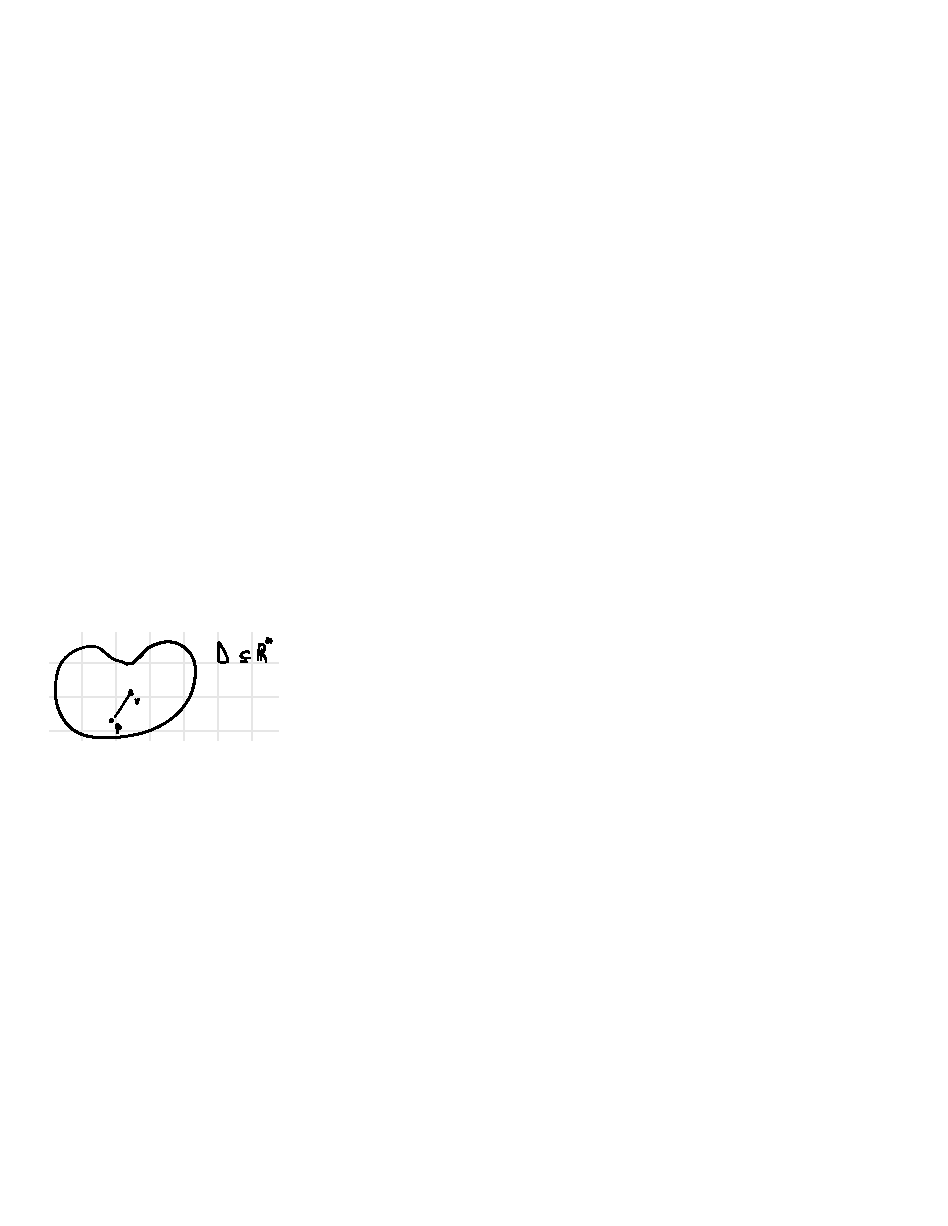
\includegraphics[width=0.5\textwidth]{img/derivate_direzionali.pdf}
	\end{figure}

	\noindent
	Si definisce la \textcolor{Red3}{\textbf{\underline{derivata direzionale}}} come:
	
	\begin{equation*}
		\dfrac{\partial f}{\partial v}\left(P\right) = \lim_{t \rightarrow 0} \dfrac{f\left(P + tv\right) - f\left(P\right)}{t}
	\end{equation*}

	\noindent
	Si descrive un'interessante osservazione:
	
	\begin{itemize}[label=\ding{42}]
		\item Se $v = \left(1,0\right)$ allora si risolve la \textbf{derivata parziale} rispetto a $x$ con $y$ costante:
		\begin{equation*}
			\dfrac{\partial f}{\partial x}\left(P\right)
		\end{equation*}
	
		\item Se $v = \left(0,1\right)$ allora si risolve la \textbf{derivata parziale} rispetto a $y$ con $x$ costante:
		\begin{equation*}
			\dfrac{\partial f}{\partial y}\left(P\right)
		\end{equation*}
	\end{itemize}

	\subsection{Nota fondamentale sulle derivate direzionali e parziali}
	
	\textbf{L'esistenza delle derivate parziali (o di tutte le derivate direzionali) in un punto \underline{non} garantisce la continuità in quel punto.}
	
	\newpage
	
	\section{Lezione 13}
	
	\subsection{Differenziabilità e funzione di Taylor}\label{differenziabilità}\label{funzione di Taylor}
	
	Una funzione $f$ definita:
	
	\begin{equation*}
		f: D \subseteq \mathbb{R}^{2} \longrightarrow \mathbb{R}
	\end{equation*}
	
	\noindent
	Si dice \textcolor{Red3}{\textbf{\underline{differenziabile}}} in un punto $\left(x_{0}, y_{0}\right)$ intorno a $D$ se esistono le derivate parziali rispetto ad $x$ e rispetto a $y$:
	
	\begin{equation*}
		\dfrac{\partial f}{\partial x}\left(x_{0}, y_{0}\right) \hspace{2em} \text{ e } \hspace{2em} \dfrac{\partial f}{\partial y}\left(x_{0}, y_{0}\right)
	\end{equation*}

	\noindent
	E se esiste anche il limite:
	
	\begin{equation*}
		\lim_{\left(x,y\right) \rightarrow \left(x_{0}, y_{0}\right)} \dfrac{f\left(x,y\right) - T\left(x,y\right)}{\sqrt{\left(x-x_{0}\right)^{2} + \left(y-y_{0}\right)^{2}}} = 0
	\end{equation*}

	\noindent
	Dove $\sqrt{\left(x-x_{0}\right)^{2} + \left(y-y_{0}\right)^{2}}$ indica la distanza tra i due punti $\left(x,y\right)$ e $\left(x_{0}, y_{0}\right)$.\newline
	
	\noindent
	Infine, la funzione è differenziabile in un punto se anche la \textcolor{Red3}{\textbf{\underline{funzione di Taylor}}} è definita nel seguente modo:
	
	\begin{equation*}
		T\left(x,y\right) = f\left(x_{0}, y_{0}\right) + \dfrac{\partial f}{\partial x}\left(x_{0}, y_{0}\right)\left(x-x_{0}\right) + \dfrac{\partial f}{\partial y}\left(x_{0}, y_{0}\right)\left(y-y_{0}\right)
	\end{equation*}

	\newpage

	\subsubsection[Esempio 1]{\textcolor{Green4}{Esempio 1}}
	
	Data la funzione:
	
	\begin{equation*}
		f\left(x,y\right) = xy - 3x^{2} \hspace{2em} \text{con } \left(x_{0},y_{0}\right) = \left(1,2\right)
	\end{equation*}

	\noindent
	Dimostrare che la funzione $f$ è differenziabile in $\left(1,2\right)$.\newline
	
	\noindent
	In primis, si \textbf{calcolano le derivate parziali}:
	
	\begin{equation*}
		\begin{array}{lll}
			\dfrac{\partial f}{\partial x}\left(x,y\right) = y - 6x & \longrightarrow & \dfrac{\partial f}{\partial x}\left(1,2\right) = 4 \\
			&& \\
			\dfrac{\partial f}{\partial y}\left(x,y\right) = x		& \longrightarrow & \dfrac{\partial f}{\partial y}\left(1,2\right) = 1
		\end{array}
	\end{equation*}

	\noindent
	Si \textbf{calcola la funzione di Taylor}:
	
	\begin{equation*}
		T\left(x,y\right) = -1 - 4\left(x-1\right) + 1\left(y-2\right)
	\end{equation*}
	
	\noindent
	Dove il $-1$ è la funzione $f\left(1,2\right)$. Si \textbf{calcola il limite}:
	
	\begin{equation*}
		\begin{array}{lll}
			\lim_{\left(x,y\right) \rightarrow \left(x_{0}, y_{0}\right)} \dfrac{f\left(x,y\right) - T\left(x,y\right)}{\sqrt{\left(x-x_{0}\right)^{2} + \left(y-y_{0}\right)^{2}}} & = & \lim_{\left(x,y\right) \rightarrow \left(1,2\right)} \dfrac{f\left(x,y\right) - T\left(x,y\right)}{\sqrt{\left(x-1\right)^{2} + \left(y-2\right)^{2}}} \\
			&& \\
			& = & \lim_{\left(x,y\right) \rightarrow \left(1,2\right)} \dfrac{xy - 3x^{2} + 1 + 4\left(x-1\right) - \left(y-2\right)}{\sqrt{\left(x-1\right)^{2} + \left(y-2\right)^{2}}}
		\end{array}
	\end{equation*}

	\noindent
	Si \textbf{calcolano le coordinate polari}:
	
	\begin{equation*}
		\begin{cases}
			x = 1 + r \cdot \cos\left(\theta\right) \\
			y = 2 + r \cdot \sin\left(\theta\right)
		\end{cases}
	\end{equation*}
	\vspace{1em}
	\begin{equation*}
		0 \le \left|\dfrac{\left(1 + r \cdot \cos\left(\theta\right)\right)\left(2 + r\cdot\sin\left(\theta\right)\right) - 3\left(1 + r\cdot\cos\left(\theta\right)\right)^{2} + 1 + 4 r \cdot \cos\left(\theta\right) - r \cdot \sin\left(\theta\right)}{\sqrt{r^{2} \cdot \cos^{2}\left(\theta\right) + r^{2} \cdot \sin^{2}\left(\theta\right)}}\right| =
	\end{equation*}
	\vspace{1em}
	\begin{equation*}
		\left|\dfrac{r \cdot \sin\left(\theta\right)\cos\left(\theta\right) - 3 r^{2} \cdot \cos^{2}\left(\theta\right)}{r}\right| = \left|\dfrac{r^{2}\left(\sin\left(\theta\right)\cos\left(\theta\right) - 3\cos^{2}\left(\theta\right)\right)}{r}\right| \le 4r
	\end{equation*}

	\noindent
	Con $4r$ che indica la funzione $g\left(r\right)$ che tende a zero con $r \rightarrow 0^{+}$.\newline
	
	\noindent
	Quindi il limite esiste ed è stato dimostrato grazie alla tecnica del confronto.
	
	\subsubsection[Nota: piano tangente]{\textcolor{Red3}{Nota: piano tangente}}
	
	Se la funzione $f\left(x,y\right)$ è differenziabile in $\left(x_{0}, y_{0}\right)$, allora l'equazione:
	
	\begin{equation*}
		z = f\left(x_{0}, y_{0}\right) + \dfrac{\partial f}{\partial x}\left(x_{0},y_{0}\right)\left(x-x_{0}\right) + \dfrac{\partial f}{\partial y}\left(x_{0},y_{0}\right)\left(y-y_{0}\right)
	\end{equation*}

	\noindent
	Definisce un piano in $\mathbb{R}^{3}$ chiamato il \textcolor{Red3}{\textbf{\underline{piano tangente}}} al grafico di $f$ nel punto $\left(x_{0},y_{0},f\left(x_{0},y_{0}\right)\right)$ con $f\left(x_{0},y_{0}\right)$ rappresenta $z_{0}$.
	
	\newpage
	
	\subsubsection[Esempio 2]{\textcolor{Green4}{Esempio 2}}
	
	Data la funzione:
	
	\begin{equation*}
		f\left(x,y\right) = ye^{-x^{2}}
	\end{equation*}

	\noindent
	Si trovi l'equazione del piano tangente nel punto in cui $x = 0, y = 1$.\newline
	
	\noindent
	Per ottenere il piano tangente si inizia con il calcolare le parti:
	
	\begin{equation*}
		f\left(x_{0}, y_{0}\right) = f\left(0,1\right) = 1
	\end{equation*}

	\noindent
	Le derivate parziali:
	
	\begin{equation*}
		\begin{array}{lll}
			\dfrac{\partial f}{\partial x}\left(x_{0},y_{0}\right) & = & \dfrac{\partial f}{\partial x}\left(0,1\right) = y \cdot \left(-2x\right)e^{-x^{2}} \Bigg|_{x=0, y=1} = 0 \\
			&& \\
			\dfrac{\partial f}{\partial y}\left(x_{0},y_{0}\right) & = & \dfrac{\partial f}{\partial y}\left(0,1\right) = e^{-x^{2}} \Bigg|_{x=0, y=1} = 1
		\end{array}
	\end{equation*}

	\noindent
	L'\textbf{equazione del piano tangente}:
	
	\begin{equation*}
		z = 1 + 0\left(x-0\right) + 1\left(y-1\right) = 1 + y - 1 = y
	\end{equation*}

	\newpage

	\subsubsection[Esempio 3]{\textcolor{Green4}{Esempio 3}}
	
	Determinare le coordinate di tutti i punti del grafico della funzione:
	
	\begin{equation*}
		f\left(x,y\right) = x^{3} - x^{2}y + y
	\end{equation*}

	\noindent
	In cui il piano tangente è orizzontale, cioè $z$ è costante.\newline
	
	\noindent
	Si inseriscono le derivate parziali nel sistema per trovare le coordinate:
	
	\begin{equation*}
		\begin{cases}
			\dfrac{\partial f}{\partial x}\left(x_{0},y_{0}\right) = 0 \\
			\\
			\dfrac{\partial f}{\partial y}\left(x_{0},y_{0}\right) = 0
		\end{cases}
		\xrightarrow{\text{Svolgendo le derivate parziali}}
		\begin{cases}
			3x^{2} - 2xy = 0 \\
			-x^{2} + 1 = 0
		\end{cases}
	\end{equation*}

	\noindent
	Risolvendo la seconda equazione, cioè $-x^{2} + 1 = 0$, si trovano le soluzioni $x = \pm 1$. Si sostituiscono i valori trovati nella prima equazione, cioè $3x^{2} - 2xy = 0$:
	
	\begin{equation*}
		\begin{array}{lll}
			\text{Caso } x = 1	& \longrightarrow &
			\begin{cases}
				x = 1 \\
				\\
				3 - 2y = 0 \longrightarrow y = \dfrac{3}{2}
			\end{cases} \\
			\\
			\text{Caso } x = -1	& \longrightarrow &
			\begin{cases}
				x = -1 \\
				\\
				3 + 2y = 0 \longrightarrow y = -\dfrac{3}{2}
			\end{cases}
		\end{array}
	\end{equation*}

	\noindent
	Quindi, i punti cercati sono:
	
	\begin{equation*}
		A\left(1, \dfrac{3}{2}, 1^{\textcolor{Red3}{\star}}\right), \hspace{2em} B\left(-1, -\dfrac{3}{2}, -1^{\textcolor{Green4}{\star}}\right)
	\end{equation*}

	Dove:
	
	\begin{itemize}[label=-]
		\item \textcolor{Red3}{$\star$} rappresenta il risultato della funzione $f\left(1,\dfrac{3}{2}\right)$
		\item \textcolor{Green4}{$\star$} rappresenta il risultato della funzione $f\left(-1, -\dfrac{3}{2}\right)$
	\end{itemize}

	\newpage
	
	\subsubsection{Nota: differenziale relativo agli incrementi}
	
	Data la funzione:
	
	\begin{equation*}
		f\left(x,y\right) = f\left(x_{0},y_{0}\right) + \dfrac{\partial f}{\partial x}\left(x_{0},y_{0}\right)\left(x-x_{0}\right) + \dfrac{\partial f}{\partial y}\left(x_{0},y_{0}\right)\left(y-y_{0}\right) + \overbracket{0\underbrace{\left(\sqrt{\left(x-x_{0}\right)^{2} + \left(y-y_{0}\right)^{2}}\right)}_{\left(x,y\right) \rightarrow \left(x_{0},y_{0}\right)}}^{\text{funzione d'errore}}
	\end{equation*}

	\noindent
	L'\textcolor{Red3}{\textbf{\underline{incremento della variabile dipendente}}}, rappresentato con $\Delta f$:
	
	\begin{equation*}
		f\left(x,y\right) - f\left(x_{0},y_{0}\right) = \underbrace{\dfrac{\partial f}{\partial x}\left(x_{0},y_{0}\right)\left(x-x_{0}\right) + \dfrac{\partial f}{\partial y}\left(x_{0},y_{0}\right)\left(y-y_{0}\right)}_{\star} + 0\left(\sqrt{\left(x-x_{0}\right)^{2} + \left(y-y_{0}\right)^{2}}\right)
	\end{equation*}

	\noindent
	In cui la $\star$ rappresenta il \textcolor{Red3}{\textbf{differenziale di $f$ in $\left(x_{0},y_{0}\right)$ relativo agli incrementi $\Delta x$ e $\Delta y$}}.\newline
	
	\noindent
	Quindi, il \textcolor{Red3}{\textbf{\underline{differenziale}}} della funzione $f$ in $\left(x_{0},y_{0}\right)$ è rappresentato da:
	
	\begin{equation*}
		\mathrm{d}f_{\left(x_{0},y_{0}\right)} : \left(\Delta x, \Delta y\right) \longrightarrow \dfrac{\partial f}{\partial x}\left(x_{0},y_{0}\right)\Delta x + \dfrac{\partial f}{\partial y}\left(x_{0},y_{0}\right) \Delta y
	\end{equation*}

	\noindent
	Esso è un'applicazione lineare da $\mathbb{R}^{2}$ a $\mathbb{R}$.
	
	\newpage
	
	\subsubsection[Esempio 4]{\textcolor{Green4}{Esempio 4}}
	
	Data la funzione:
	
	\begin{equation*}
		f\left(x,y\right) = \sqrt{2x^{2} + e^{2y}}
	\end{equation*}

	\noindent
	Calcolare un valore approssimato della funzione $f$ in $\left(2.2, -0.2\right)$.\newline
	
	\noindent
	Il punto $\left(2.2, -0.2\right)$ è vicino a $\left(2, 0\right)$. Quindi, bisogna calcolare l'incremento:
	
	\begin{equation*}
		f\left(2.2,-0.2\right) - f\left(2,0\right)
	\end{equation*}

	\noindent
	Che corrisponde in modo approssimato a:
	
	\begin{equation*}
		\Delta f \approx f_{\left(2,0\right)} \left(0.2,-0.2\right) = \dfrac{\partial f}{\partial x}\left(2,0\right) \cdot 0.2 + \dfrac{\partial f}{\partial y}\left(2,0\right) \cdot \left(-0.2\right)
	\end{equation*}

	\noindent
	I valori $0.2$ e $-0.2$ rappresentano gli incrementi delle variabili $x$ e $y$:
	
	\begin{equation*}
		\begin{array}{llllll}
			x: & 2 & \rightarrow & \phantom{-}2.2	& \xrightarrow{\text{incremento effettuato}} & \phantom{-}0.2 \\
			y: & 0 & \rightarrow & -0.2				& \xrightarrow{\text{incremento effettuato}} & -0.2
		\end{array}
	\end{equation*}

	\noindent
	Si \textbf{calcolano le derivate parziali}:
	
	\begin{equation*}
		\begin{array}{lllll}
			\dfrac{\partial f}{\partial x}\left(x,y\right) & = & \dfrac{1}{2\sqrt{2x^{2} + e^{2y}}} \cdot 4x		& \longrightarrow & \dfrac{\partial f}{\partial x}\left(2,0\right) = \dfrac{4}{3} \\
			&&&& \\
			\dfrac{\partial f}{\partial y}\left(x,y\right) & = & \dfrac{1}{2\sqrt{2x^{2} + e^{2y}}} \cdot 2e^{2y}	& \longrightarrow & \dfrac{\partial f}{\partial y}\left(2,0\right) = \dfrac{1}{3}
		\end{array}
	\end{equation*}

	\noindent
	Per concludere, l'incremento della funzione passando dal punto $\left(2,0\right)$ a $\left(2.2,-0.2\right)$ è circa:
	
	\begin{equation*}
		\Delta f \approx \dfrac{4}{3} \cdot 0.2 - \dfrac{1}{3} \cdot 0.2 = 0.2
	\end{equation*}

	\noindent
	E dunque la funzione valutata in $\left(2,0\right)$ vale $3$ e si termina scrivendo:
	
	\begin{equation*}
		f\left(2.2,-0.2\right) \approx 3 + 0.2 = 3.2
	\end{equation*}

	\newpage
	
	\subsection{Gradiente}
	
	Se la funzione $f$ ammette derivate parziali in $\left(x_{0},y_{0}\right)$ il vettore:
	
	\begin{equation*}
		\nabla f\left(x_{0},y_{0}\right) = \left(\dfrac{\partial f}{\partial x}\left(x_{0},y_{0}\right), \dfrac{\partial f}{\partial y}\left(x_{0},y_{0}\right)\right)
	\end{equation*}

	\noindent
	Si chiama \textcolor{Red3}{\textbf{\underline{gradiente}}} di $f$ in $\left(x_{0},y_{0}\right)$ (il simbolo $\nabla$ si legge \emph{nabla}).\newline
	
	\noindent
	Grazie al gradiente è possibile riscrivere qualche formula:
	
	\begin{itemize}
		\item \textcolor{Red3}{\textbf{\underline{Funzione di Taylor}}} (pagina \pageref{funzione di Taylor}):
		\begin{equation*}
			T\left(x,y\right) = f\left(x_{0},y_{0}\right) + \nabla f\left(x_{0},y_{0}\right) \cdot \left(x-x_{0},y-y_{0}\right) \hspace{2em} \text{N.B. è un prodotto scalare}
		\end{equation*}
	
		\item \textcolor{Red3}{\textbf{\underline{Differenziale}}} (pagina \pageref{differenziabilità}):
		\begin{equation*}
			\mathrm{d}f_{\left(x_{0},y_{0}\right)}\left(\Delta x, \Delta y\right) = \nabla f\left(x_{0},y_{0}\right) \cdot \left(\nabla x, \nabla y\right) \hspace{2em} \text{N.B. è un prodotto scalare}
		\end{equation*}
		Una notazione alternativa del prodotto scalare può essere la seguente:
		\begin{equation*}
			\left\langle \nabla f\left(x_{0}, y_{0}\right), \left(\Delta x, \Delta y\right) \right\rangle
		\end{equation*}
	\end{itemize}

	\newpage
	
	\subsection{Generalizzazione del concetto di differenziabilità per funzioni di $\boldsymbol{n}$ variabili}
	
	Sia la funzione $f$ definita in un intorno di $\bar{x} \in \mathbb{R}^{n}$ e supponiamo che esistano tutte le derivate parziali di $f$ in $\bar{x}$. Si dice che $f$ è \textbf{differenziabile} in $\bar{x}$ se:
	
	\begin{equation*}
		\lim_{x \rightarrow \bar{x}} \dfrac{f\left(x\right) - T\left(x\right)}{\Big||x-\bar{x}|\Big|} = 0 \hspace{1em} \text{con } T\left(x\right) = f\left(\bar{x}\right) + \dfrac{\partial f}{\partial x_{1}}\left(\bar{x}\right) \cdot \left(x_{1} - \bar{x}_{1}\right) + \cdots + \dfrac{\partial f}{\partial x_{n}}\left(\bar{x}\right) \cdot \left(x_{n} - \bar{x}_{n}\right)
	\end{equation*}

	\noindent
	Dove la parte di derivate parziali rappresenta il differenziale di $f$ in $\bar{x}$ relativo agli incrementi $\Delta x_{i}$ con $i = 1, ..., n$:
	
	\begin{equation*}
		\sum_{i = 1}^{n} \dfrac{\partial f}{\partial x_{i}}\left(\bar{x}\right)\left(x_{i} - \bar{x}_{i}\right)
	\end{equation*}

	\noindent
	Il \textbf{gradiente} è:
	
	\begin{equation*}
		\nabla f\left(\bar{x}\right) = \left(\dfrac{\partial f}{\partial x_{1}}\left(\bar{x}\right), \cdots, \dfrac{\partial f}{\partial x_{n}}\left(\bar{x}\right)\right)
	\end{equation*}

	\subsection[Teorema: differenziabilità implica continuità]{\textcolor{Red3}{Teorema: differenziabilità implica continuità}}
	
	\begin{theorem}[\textbf{Differenziabilità implica continuità}]\label{teorema: differenziabilità implica continuità}
		Se la funzione $f$ è differenziabile nel punto $x_{0}$, allora la funzione $f$ è continua nel punto $x_{0}$. Quindi, in altre parole, la differenziabilità implica la continuità.
	\end{theorem}

	\subsection[Teorema: differenziale totale]{\textcolor{Red3}{Teorema: differenziale totale}}
	
	\begin{theorem}[\textbf{Differenziale totale}]\label{teorema: differenziale totale}
		Se una funzione $f$ ammette tutte le derivate parziali in un intorno di $x_{0}$ interno la dominio di $f$, continua in $x_{0}$, allora $f$ è differenziabile.
	\end{theorem}

	\newpage
	
	\subsubsection[Esempio]{\textcolor{Green4}{Esempio}}
	
	Data la funzione:
	
	\begin{equation*}
		f\left(x,y\right) = \sqrt{x^{2} + y^{2}} \hspace{2em} \text{con } D_{f} = \mathbb{R}^{2}
	\end{equation*}

	\noindent
	Si \textbf{calcolano le derivate parziali}:
	
	\begin{equation*}
		\begin{array}{lll}
			\dfrac{\partial f}{\partial x}\left(x,y\right) & = & \dfrac{x}{\sqrt{x^{2} + y^{2}}} \\
			&& \\
			\dfrac{\partial f}{\partial y}\left(x,y\right) & = & \dfrac{y}{\sqrt{x^{2} + y^{2}}}
		\end{array}
	\end{equation*}
	
	\noindent
	Le funzioni sono continue in $\mathbb{R}^{2} \setminus \left\{0,0\right\}$, quindi grazie al teorema a pagina~\pageref{teorema: differenziabilità implica continuità}, la funzione $f$ è differenziabile in tutti i punti di $\mathbb{R}^{2}$ escluso $\left(0,0\right)$.\newline
	
	\noindent
	\textcolor{Red3}{\textbf{\emph{La funzione $f$ è differenziabile in $\left(0,0\right)$?}}}\newline
	
	\noindent
	La risposta è no. Infatti, calcolando la derivata parziale rispetto a $x$ tramite la definizione:
	
	\begin{equation*}
		\dfrac{\partial f}{\partial x}\left(0,0\right) = \lim_{h \rightarrow 0} \dfrac{\sqrt{h^{2} + 0} - 0}{h} = \lim_{h \rightarrow 0} \dfrac{\sqrt{h^{2}}}{h} = \lim_{h \rightarrow 0} \dfrac{\left|h\right|}{h}
	\end{equation*}

	\noindent
	Le soluzioni sono $+1$ con $h \rightarrow 0^{+}$ e $-1$ con $h \rightarrow 0^{-}$.\newline
	
	\noindent
	Quindi \textbf{non esistono le derivate parziali} di $x$ e $y$ nel punto $\left(0,0\right)$, ovvero non esiste in:
	
	\begin{equation*}
		\dfrac{\partial f}{\partial x}\left(0,0\right) \hspace{1em} \text{ e } \hspace{1em} \dfrac{\partial f}{\partial y}\left(0,0\right)
	\end{equation*}
\end{document}